\documentclass[a4paper,12pt]{article}
%\documentclass[12pt]{article}
\usepackage{setspace}  % Add this line to use the setspace package
\usepackage{times} % For time new roman font style
% Packages
\usepackage[a4paper, margin=1in]{geometry}
\usepackage{fancyhdr}
\usepackage{graphicx}
\usepackage{lipsum}
\usepackage{xcolor}
\usepackage{setspace}
\usepackage{eso-pic}
\usepackage{titlesec}
\usepackage{tikz}
\usepackage{graphicx}
\usepackage{float}

% Load necessary packages

\usepackage{setspace}
\usepackage{sectsty}
\usepackage{enumerate}
% \usepackage{ragged2e}
\usepackage{afterpage} %% For longtable forcing on a particular page 

%\usepackage{microtype}
%\usepackage[none]{hyphenat} % To remove automatic words breaks due to justify alignment

\usepackage{circuitikz}
\usepackage{tikz}

\usepackage{csvsimple}
\usepackage{siunitx} %% My regression reult with model summary

\usepackage{longtable}
\usepackage{tabularx}
%\usepackage{ltablex}
\usepackage{pdflscape}
\usepackage{subcaption} % Combining Tables
\usepackage{booktabs} %%% For table formatting
%\usepackage{multirow} % Not useful. Dont like it 
\usepackage{array}  % <-- Include the array package
\usepackage{caption} % For Caption

\usepackage{amsmath}
\usepackage{amssymb}

%%% Landscape pages 
%\usepackage{lscape}
%\usepackage{pdflscape}
\usepackage{rotating}


\usepackage[absolute,overlay]{textpos}
\usepackage{microtype} % to prevent hyphenated words 

\usepackage{sectsty}
\allsectionsfont{\normalsize}
%\usepackage[rm,tiny]{titlesec}
%in the preamble
%--------------------------------
\usepackage[hidelinks]{hyperref}  % Add the hyperref package with hidelinks option

\usepackage[backend=biber, style=apa, sorting = nyt]{biblatex}
\addbibresource{Reference.bib}
% Header and Footer
\pagestyle{fancy}
\fancyhf{}

%\fancyhead[R]{\rule{\textwidth}{1pt}} % Horizontal line under the logo
\fancyfoot[C]{\thepage}
\renewcommand{\headrulewidth}{0pt}
\renewcommand{\footrulewidth}{0pt}
%\fancyhead[L]{
\includegraphics[height=1.5cm]{Figures/HBRS.png}} % Add your university logo
% Define a custom color
%\definecolor{myblue}{RGB}{0,0,128}


% Set font size to 12pt for the document
%\renewcommand{\normalsize}{\fontsize{12}{15}\selectfont}


% Customize section and subsection headings
\sectionfont{\fontsize{16}{16}\selectfont\bfseries} % Section headings: 14pt bold
\subsectionfont{\fontsize{13}{15}\selectfont\bfseries} % Subsection headings: 13pt bold



\pagestyle{fancy}
\fancyhf{} % Clear header and footer settings
\rfoot{\thepage} % Right-aligned page number
\renewcommand{\headrulewidth}{0pt} % Remove header line
\renewcommand{\footrulewidth}{0.4pt} % Footer line thickness
\renewcommand{\footnoterule}{\hrule width\textwidth} % Full-width footer line




%https://www.researchgate.net/post/What_assumptions_need_to_be_tested_before_performing_a_fixed_effect_regression_on_panel_data
% Interpretation and identification of within-unit and cross-sectional variation in panel data model Jonathan Kropko ,Robert Kubinec  

% Preliminary pages with Roman numerals
\pagenumbering{roman}


\tolerance = 1
\emergencystretch = \maxdimen
\hyphenpenalty = 10000
\hbadness = 10000


%{\tiny \scriptsize \footnotesize \small \normalsize \large \Large \LARGE \huge \Huge} For different font size

\begin{document}



% Your document content goes here




%--------------------------------

%\onehalfspacing % Set 1.5 line spacing

% Preliminary Pages

    
\begin{titlepage}

% Position the university logo
\begin{tikzpicture}[remember picture, overlay]
  \node[anchor=north west, inner sep=17pt] at ([xshift =1cm] current page.north west) {
\includegraphics[width=9cm]{Figures/HBRS.png}};
\end{tikzpicture}


    \begin{textblock*}{6cm}(13cm, 1cm) % Adjust the values as needed
    \raggedright
        {\fontsize{11}{12}{\sffamily Department of \\
        Social Policy and Social Security \\ Studies}}
   \end{textblock*}


   

\vspace*{3cm}
\centering
{\fontsize{20}{12} \textbf{Master Thesis}}

\vspace*{1.5cm}

    {\fontsize{16}{12}To obtain the degree \\
Master of Scienece (M.Sc.) in Social Protection}


\vspace*{4cm}

\begin{onehalfspace}
{\fontsize{15}{12} \textbf{ \textit{Evaluating the Impact of Foreign Aid on Health Outcomes in Developing Countries: An Empirical Comparison of Sub-Saharan Africa (SSA) and Non-SSA Regions}}}
    
\end{onehalfspace}

\vspace*{3cm}

{\flushleft
\begin{tabular}{l l}

Submitted by:     & \quad \textit{Olowookere, Oluwatosin Olawale} \\
  Matriculation No:   & \quad \textit{9048167} \\
  Email: & \quad  \href{mailto:Olowookere Oluwatosin}{\textit{olowookereolwale1993@gmail.com}}\\
Date of Submission: & \quad  \textit{\today}\\
  
  \vspace*{12pt}\\
1st Supervisor: & \quad  \textit{Prof. Axel Weber}\\
Institution         & \quad  \textit{Department of Social Policy and Social Security Studies}\\ 
        &                      \quad \textit{Hochschule Bonn-Rhein-Sieg (HBRS) University of Applied Sciences}\\
        
E-mail & \quad  \href{mailto:Weber Axel}{\textit{Axel.Weber@h-brs.de}}

\vspace*{12pt}\\
2nd Supervisor:		& \quad  \textit{Prof. Krystof Hagemejer}\\
Institution         & \quad  \textit{Department of Social Policy and Social Security Studies}\\ 
        &                      \quad \textit{Hochschule Bonn-Rhein-Sieg (HBRS) University of Applied Sciences}\\
E-mail  & \quad  \href{mailto:krzysztof.hagemejer@h-brs.de}{\textit{krzysztof.hagemejer@h-brs.de}}\\

\end{tabular}











%Submitted by: 		\quad \quad \quad  \textit{Olowookere, %Oluwatosin Olawale} \par
%Matriculation No:	\quad \quad  \textit{9048167} \par
%Email:			\quad \quad \quad  \textit{olowookereolwale1993@gmail.com} \par
%Date of Submission:	\quad \quad  \textit{15.03.1993} \par

%\vspace*{12pt}
%1st Supervisor:		\quad \quad  \textit{Prof. Axel Weber} \par
%Institution          \quad \quad  \textit{Hochschule Bonn-Rhein-Sieg (HBRS)} \par
%E-mail               \quad \quad  \textit{\ Axel.Weber@h-brs.de} \par

\vspace*{12pt}

%2nd Supervisor:		\quad \quad  \textit{Prof. Krystof Hagemejer} \par
%Institution         \quad \quad  \textit{Hochschule Bonn-Rhein-Sieg (HBRS)} \par

%E-mail  \quad \quad  \href{mailto:krzysztof.hagemejer@h-brs.de}{\textit{krzysztof.hagemejer@h-brs.de}} \par
}

\end{titlepage}


\begin{onehalfspace}


%%%%%%%%%% Declaration Statement and Oat page %%%%%%%%%%%%%%%%%%%%%%
\section*{\centering Statement Lieu of Oath}
\flushleft
%\begin{doublespace}
I hereby declare that I have authored this Master’s Thesis independently, that I have not used other sources/resources than the ones declared, and that I have explicitly marked all material which has been quoted either literally or by content from the used sources. According to my knowledge, the content or parts of this Master’s Thesis has not been presented to any other examination authority and have not been published. I am aware that the respective work can be considered as a "fail" in the event of a false declaration.

\vspace*{12pt}
I understand that the Master’s Thesis will be scanned for plagiarism with the help of “Turnitin”, “Docoloc” or any other plagiarism detection software. By uploading the Master’s Thesis to LEA I automatically agree to its storage to the repository to enable comparison with future exams/papers submitted.

\vspace*{12pt}
This declaration does not grant the Hochschule Bonn-Rhein-Sieg permission to reproduce, publish or use this exam/paper without my consent. In any case, the examination and evaluation of my work must be carried out individually and independently from the results of the plagiarism detection service.

\vspace*{12pt}
\textit{Attention: Please fill in and sign the document, do not change the name of the file and upload it separately to LEA.  If this document is missing, your Master’s Thesis will not be reviewed and will therefore be considered as failed.}


\vspace*{4cm}
\rule{\textwidth}{0.4pt}\\
%\vspace*{pt}

\quad Date/Place	\hspace{6cm}   Name



\vspace*{3cm}

\rule{7cm}{0.4pt}\\
\quad Matriculation Number
%\end{doublespace}




\section*{\centering Acknowledgement}
\addcontentsline{toc}{subsection}{Acknowledgement}

I extend my sincere gratitude to those who have been instrumental in my academic journey, especially in the successful completion of this thesis. I am deeply thankful to my two supervisors, Prof Axel Weber (first supervisor) and Prof Hagemejer (second supervisor), for their unwavering support, insightful comments, and valuable feedback. Their guidance not only strengthened my courage but also facilitated the timely completion of this thesis. 


I am equally thankful to the entire staff of the Department of Social Policy and Social Security Studies. Particularly, I am appreciate Prof. Hellsmuller Simona, the current head of the M.Sc. in Social Protection programme, for her mentoring all through the course of this master programme. Special acknowledgment goes to the in-house DAAD advisor, Mr Abdulraman, and the thesis coordinator, Mr Brian, for their support and openness.

 

My gratitude extends to the HBRS university writing center, particularly to Prof Yates Jill, for her tenacious support and insightful comments despite a demanding schedule. I must acknowledge Mrs Christiana Loewe for her encouraging words during the challenging phases of this journey. Your collective contributions have been invaluable, and I am deeply thankful for the rewarding experiences gained through our interactions   

\renewcommand{\contentsname}{\centering Table of Contents} % Rename the contents title

\linespread{1.5} % Adjust the line spacing (e.g., 1.5 for 1.5x spacing)
%\setstretch{1.25} % Adjust the value to set the line spacing
\setcounter{tocdepth}{3} % Set the depth of the table of contents
\tableofcontents
\clearpage % Start content on a new page



%\section*{\textbf{Table of Content}}



%\tableofcontents  % Generates the clickable table of contents

% Your content for Chapter One

%\section*{Chapter Two}
%\addcontentsline{toc}{section}{Chapter Two}
% Your content for Chapter Two

%\section*{Chapter Three}
%\addcontentsline{toc}{section}{Chapter Three}
% Your content for Chapter Three

% ... Continue with your document


\renewcommand{\listfigurename}{\centering List of Figures}
\listoffigures
\addcontentsline{toc}{subsection}{List of Figures}
% Rename the list of tables title
\renewcommand{\listtablename}{\centering List of Tables}

\listoftables
\addcontentsline{toc}{subsection}{List of Tables}
\section*{\centering Abstract}
\addcontentsline{toc}{subsection}{Abstract}
%The impact of health, particularly on human capital development and upholding human right, has been emphasized for several decades. Despite the global commitment to universal health exemplified in the past millenium development goals (MDGs) and the ongoing sustainable development goals (SDG), health problems remains a significant challenge in the developing countries. Some attributed such development deficit to lack of enough resources in the poor nations, making a case for foreign aid (ODA) and the need for its effectiveness. Yet past studies assessing the ODA effectiveness on health have often employed narrow health indicators. Against this backdrop, the thesis assesses the effectiveness of ODA using comprehensive composite health dimensions from SGD 2.4 on malnutrition and SDG 3 on health. The thesis also sought to understand the mediating role of social protection in such impact. The study employs a combination of panel and dynamic econometric approaches, Specifically the novel approach fixed effect cross-lag panel model (FE-CLPM), unit fixed effect and local projection, with 144 countries data between 2000 to 2021, mean aggregated into 5 periods with both total net ODA and social infrastructure ODA. Despite the variations observed in the ODA impact across health dimensions, all models reveals both total and social infrastructure ODA has significant effect on reproductive fatality, infection and diseases as well as environmental death. Moreover, findings reveals no evidence that ODA improves health system capacity nor does the impact of ODA across all health dimensions mediated by social protection or different across regions. Disparities in studies, including this thesis, could be attributed econmetrics approache employed, control variables, specific health indicators and type of ODA employed. Therefore, the thesis concludes that ODA, particularly when targeted to social infrastructure ODA, significantly influences health outcome. Enhancing health system capacity in developing countries should be the paramount focus of global development effort. This could be ensured by strengthening ODA monitoring mechanisms as well as holding recipient government responsible for mismanagement.


%Key words: Official Development Assistance (ODA or Foreign Aid), Social Protection, Health Outcomes, dynamic panel model. 





The imperatives of health in human capital development and the promotion of human rights has been emphasized for decades. Despite global commitments to universal health, as evident in the Millennium Development Goals (MDGs) and the ongoing Sustainable Development Goals (SDGs), health challenges persist in developing countries. This deficit is often attributed to resource limitations in poorer nations, prompting a reliance on Foreign Aid (ODA) to address these issues. However, previous studies assessing ODA's impact on health have predominantly utilized narrow indicators. Against this backdrop, this thesis evaluates ODA effectiveness by employing comprehensive composite health dimensions created from SDG 2 (malnutrition) and SDG 3 (health and well-being). Additionally, it explores the mediating role of social protection in this impact. Utilizing a combination of panel econometric approaches, including the fixed effect cross-lag panel model (FE-CLPM), unit fixed effect, and local projection, the study analyzes data from 144 countries spanning 2000 to 2021, mean aggregated into five periods, considering both total net ODA and social infrastructure ODA. Despite observed variations in ODA impact across health dimensions, all models reveal significant effects of both total and social infrastructure ODA on reproductive fatality, infection and diseases, as well as environmental death. Findings, however, suggest no evidence that ODA improves health system capacity, nor does its impact across health dimensions mediated by social protection or differ significantly between SSA and non-SSA regions. Discrepancies in study outcomes, including this thesis, may be attributed to differences in econometric approaches, control variables, specific health indicators, and types of ODA employed. Consequently, the thesis concludes that ODA, especially when directed towards social infrastructure, significantly influences health outcomes. Emphasizing the enhancement of health system capacity in developing countries should be a primary focus of global development efforts. This necessitates strengthening ODA monitoring mechanisms and holding recipient governments accountable for mismanagement.

\vspace{10pt}
\textbf{Keywords}: Official Development Assistance (ODA or Foreign Aid), Social Protection, Health Outcomes, Composite health dimension, Dynamic Panel Model, Fixed Effect Cross-Lag Panel Model (FE-CLPM), 


\end{onehalfspace}
% Your content goes here




%\begin{onehalfspace}  % Use the onehalfspace environment 


%\begin{doublespace}  % Use the doublespace environment for double line spacing

% Switch to Arabic page numbering for main content
\clearpage
\pagenumbering{arabic}

%{\justify

\begin{onehalfspace}
    
% Chapters and Sections
% Note that you can not nest include function, but you can use input in the included document
\section*{\centering Chapter One}
\section*{\centering Introduction}
%\addcontentsline{toc}{section}{Chapter One}
\addcontentsline{toc}{section}{Chapter One: Introduction}
% Your introduction content goes here

\subsection*{1.1 \quad Study Background} 
\addcontentsline{toc}{subsection}{1.1	Background of the Study}

Health plays a crucial role in human capital development, upholding fundamental rights, and fostering economic growth \parencite{yogo_health_2015}. This perspective, especially regarding the centrality of health capital in economic development, has been extensively discussed by endogenous growth theorists \textcite{grossman_concept_1972, ostlin_paying_2004, sen_health_1998} amongst others. They argue that a healthy population is a productive one, emphasizing the reciprocal relationship between health and wealth. Despite the significance of this, developing nations continue to face persistent health challenges \parencite{gama_health_2015}, despite decades of global health initiatives. This has become particularly important in the present era of Sustainable Development Goals (SDGs), with SDG 3 dedicated to advancing Universal Health Coverage (UHC) and the overall well-being of all people.

In recent decades, international organizations such as the International Labour Organization (ILO), World Health Organization (WHO), and World Bank have increasingly highlighted the role of social protection in ensuring health security in developing countries. According to these organizations, social protection acts as a potential tool for poverty eradication and reduction, improving access and affordability, and eliminating financial barriers to health services \parencite{fox_clinical_2015, who_world_2010}. The ILO Social Protection Floor (SPF), for example, includes health as a basic and irreducible right for every human \parencite{ilo_social_2012, ilo_towards_2020}. This perspective aligns with the World Bank's social safety net initiative and WHO's Universal Health Coverage (UHC), highlighting the relevance of social protection to health \parencite{jorgensen_social_2019, lonnroth_beyond_2014, siroka_association_2016, who_world_2010}. In the post-COVID-19 era, the nexus between social protection and health is evident \parencite[see][]{yokobori_roles_2023}. Studies consistently highlight social protection's dual impact on public health, emphasizing a rights-based approach and contributing to health financing through social security and assistance \parencite{hagemejer_role_2013, ilo_towards_2020, macnaughton_decent_2010, yokobori_roles_2023, scheil-adlung_response_2014, scheil-adlung_focusing_2020}.

However, achieving adequate health outcomes demands substantial capital investment, posing challenges for developing nations with limited resources \parencite{world_bank_high-performance_2019}. A World Bank report indicates an annual financing gap of \$176 billion USD for UHC in the world's poorest countries by 2030 \parencite{world_bank_high-performance_2019}. Consequently, foreign aid, or Official Development Assistance (ODA), has become crucial as an alternative investment capital to address these deficits, including health-related challenges \parencite{sachs_case_2014, yogo_health_2015}. 


ODA, together with remittances, and foreign direct investment (FDI), serve as crucial channels for foreign currency flow in developing countries \parencite{scott_lessons_2020}. The OECD defines ODA as concessional loans and grants from affluent nations to foster economic growth and enhance well-being in developing countries \parencite{oecd_ODA_Report_2023} \footnote{Since 2017, the official methodology for ODA classification has changed to only consider grant equivalent flow as ODA \parencite{oecd_ODA_Report_2023}}. The effectiveness of aid in influencing diverse developmental outcomes, including economic growth, health, and social protection, has been a focal point in academic and policy discussions for decades. Debates on aid effectiveness trace back to economists such as \textcite{bauer_dissent_1979, easterly_elusive_2002, milton_foreign_1958, sachs_geography_2001}, with diverse perspectives, who are categorized into aid optimists and pessimists \parencite{kavanagh_governance_2019, nwude_official_2020}.

Aid optimists emphasize capital investment, mobilized through domestic savings and technologies, for government-led developmental purposes. The absence or inadequacy of these resources, encompassing financial, technological, and knowledge aspects, underscores the need for ODA \parencite{sachs_development_2005}. Conversely, pessimists point to persistent poverty in Africa and many parts of South Asia despite decades of ODA \parencite[see][]{yontcheva_macroeconomic_2006}. They argue that foreign aid contributes to uneven income distribution, fosters inequality, endangers governance, creates dependency, and is sometimes exploited as a pretext for foreign invasion \parencite{easterly_can_2003, easterly_are_2007, easterly_can_2009, milton_foreign_1958, easterly_elusive_2002}. Pessimists conclude that foreign aid has no positive effect or may indeed have a negative influence in developing countries \parencite{yontcheva_macroeconomic_2006}.


Subsequent scholars have elaborated on the conditions moderating or mediating aid effectiveness, leading to studies emphasizing non-linearity and context conditionality \parencite[see]{yontcheva_macroeconomic_2006}. Debates on foreign aid (or ODA) persist, especially given the rising awareness of interconnections in development challenges, exemplified by global health issues like COVID-19. This awareness has led to increased bilateral ODA allocation towards global public goods, such as public health \parencite{cepparulo_responses_2016, kenny_official_2020}, and renewed global actions on foreign aid effectiveness \parencite{cassola_evaluating_2022, ogbuoji_aid_2018} \footnote{Global actions on aid effectiveness include the Paris Declaration for Aid Effectiveness 2005, the International Health Partnership Plus 2007, the Accra Agenda for Action 2008, the Busan Partnership for Effective Corporation 2011, the Global Partnership for Effective Development Corporation (GPEDC) 2011, the 2015 Financing for Development conference of Addis Ababa Agenda (AAA), Agenda 2030, Sustainable Development Goals 2015 until 2030, and UHC in 2005 (Ibid).}. In light of these developments, the study assesses the impact of foreign aid on health outcomes and the potential mediating role of social protection in developing countries.

%\vspace{4pt}
\subsection*{1.2 \quad	Problem Statement}
\addcontentsline{toc}{subsection}{1.2 	Problem Statement}
Numerous studies have examined the influence of foreign aid on various development indicators, encompassing economic growth, health outcomes, social protection, and environmental efficiency \parencite{cassola_evaluating_2022, easterly_can_2009, milton_foreign_1958, nino-zarazua_aids_2023, nwude_official_2020, yan_mortality_2015}. However, the existing evidence remains inconclusive, with studies broadly categorized into aid pessimists and optimists \parencite{kavanagh_governance_2019, nwude_official_2020}. Optimists argue for the efficacy of foreign aid, highlighting its potential impact on developing countries' conditions in the absence of such aid \parencite{sachs_case_2014}. Studies supporting this view demonstrate that foreign aid effectively promotes economic growth, either directly or indirectly, by enhancing human development, including health security, education, and poverty reduction \parencite{bavinger_relationship_2017, doucouliagos_health_2021, marty_taking_2017, mohamed_foreign_2017}.

Conversely, aid pessimists assert that aid dependency and undue donor influence negate the anticipated benefits of foreign aid \parencite{easterly_are_2007}. Consequently, some studies reveal the ineffectiveness of foreign aid across various health and social development indicators \parencite{ali_foreign_2020, chung_economic_2022, williamson_foreign_2008}. However, others emphasize nuanced conditions moderating aid effectiveness, such as the quality of governance, economic growth, initial development levels in recipient countries \parencite{kavanagh_governance_2019, ogbuoji_aid_2018, shafa_assessment_2023}, and donor-imposed conditions \parencite{nwude_impact_2023}. Despite ongoing discussions, notable gaps persist in previous studies, raising concerns about the credibility of their findings. 

One significant gap is the reliance on health ODA as the primary predictor of health outcomes, neglecting the broader impact of ODA across various sectors and subsectors. This results in the possible underestimation of aid effectiveness, as health ODA represents only a small fraction of the social infrastructure sector.  Moreover, ODA allocated to other sectors and subsectors like climate change, education, population, and reproductive health may exert both direct and indirect influences on overall population health outcomes (see Appendix A Figure \ref{fig:General ODA classification} for OECD's ODA markers). To address this limitation, the thesis combines both total ODA and the social infrastructure sector, providing a more comprehensive assessment. 

%One significant gap is the predominant reliance on health ODA as the primary predictor of health outcomes in previous studies. This approach overlooks the broader impact of ODA distributed across various sectors and subsectors, resulting in underestimation of aid effectiveness. For example, health ODA is a small fraction of the social infrastructure sector, as shown in Appendix Figure \ref{fig:Sector ODA classification}). Moreover, ODA allocated to other sectors and subsectors like climate change, education, population, and reproductive health may exert both direct and indirect influences on overall population health outcomes (see Appendix A Figure \ref{fig:General ODA classification} for OECD's ODA markers). Since using only health ODA may underestimate the impact of interest, the thesis combines both the total ODA and the social infrastructure sector, rather than exclusively considering the health subsector, for a more comprehensive assessment.

Another gap is the choice of indicators for the endogenous variable (health outcome). Since health situations may vary in nature and intensity across regions and countries, as discussed extensively in Chapter Two, using single health metrics such as maternal mortality, malaria incidence and child mortality, may not align with the public health priorities of ODA recipient countries. Such variation could potentially lead to aid diversion \parencite{ogbuoji_aid_2018}. Aid fungibility and the context-specific nature of health problems might introduce bias when comparing countries solely on narrow health indicators. One country, for instance, may allocate ODA to child immunization, improving child health outcomes, while another may focus on adult health. This diversity may not be adequately captured by using a single indicator. Moreover, some indicators respond to changes in ODA more than others \parencite{doucouliagos_health_2021},  thus, the nature of findings may be constrained by incomprehensive indicators. To address these challenges, the thesis combines various indicators from SDG 3 on health and SDG 2 on malnutrition, to capture variations in health problems and burdens across regions, age groups, and genders. The indicators are used to construct comprehensive composite health dimensions \footnote{Please see Chapter Two for a discussion on health dimensions. The procedure for creating such dimensions is described in Appendix A.2} for a broader perspective on health outcomes across all countries.

Finally, understanding the mechanisms through which ODA impacts health outcomes remains a significant gap in the existing literature. Even among studies revealing the positive effects of ODA on health outcomes, none of these studies have explored how these effects manifest, except \parencite[]{yogo_health_2015}. This becomes particularly crucial in the era of Sustainable Development Goals (SDGs), where comprehending the mechanisms of policy intervention is paramount for optimal resource allocation. Moreover, social protection has become a key policy instrument to advance universal health coverage globally.  Against this backdrop, the thesis aims to address the following research questions:



%\vspace{1pt}

\subsection*{1.3 Research Questions}
\addcontentsline{toc}{subsection}{1.3	Research Questions}

\subsubsection*{1.3.1	Primary Research Questions:}
\addcontentsline{toc}{subsubsection}{1.3.1 	Primary Research Questions}

What is the overall effectiveness and impact of foreign aid, specifically Official Development Assistance (ODA), on health outcomes in developing countries? This overarching research question aims to investigate the comprehensive impact of ODA on diverse composite health dimensions created from relevant SDG 2 and 3 indicators. 
\subsubsection*{1.3.2	Specific Research Questions:}
\addcontentsline{toc}{subsubsection}{1.3.2 	Specific Research Questions:}
\begin{enumerate}
    \item What is the direct impact of ODA on health outcomes? This question seeks to understand the direct influence of ODA on health outcomes without the mediation of any third-party variable.
    \item Are there regional variations in the impact of ODA on health outcomes, particularly in SSA and non-SSA regions? This question aims to understand potential regional-specific effects moderating the effectiveness of ODA on health outcomes. The study seeks to determine whether adjusting for regional characteristics, primarily SSA and non-SSA, affects the pattern of foreign aid impact on various health dimensions. 
    \item Is the impact of ODA on health outcomes mediated by social protection development in developing nations? This question aims to explore whether social protection development plays a mechanistic role in the effect of ODA on health outcomes. The implication is that allocating more ODA to social protection could yield dual benefits in poverty eradication and health security.
\end{enumerate}

%\vspace{1pt} 
\subsection*{1.4	Significance of the study}
\addcontentsline{toc}{subsection}{1.4 	Significance of the study}
This thesis significantly contributes to the fields of health economics, social protection, and development studies, offering fresh insights and advancements in several key areas:
\begin{enumerate}[i]
    \item Knowledge and empirical implications: 
    \begin{itemize}
        \item Conceptual Broadening: While previous research has investigated aid effectiveness on narrow health indicators, this study distinguishes itself by broadening the concept of health outcomes. Unlike previous studies that use narrow indicators as proxies for the complex and multidimensional construct of health outcomes, this research constructs diverse composite health dimensions from SDG 2 on malnutrition and SDG 3 on health and human well-being. By including indicators from SDG 2, such as child stunting, women’s anaemia, and incidence of malnutrition, the study ensures a comprehensive understanding of health outcomes. This approach facilitates inter-regional comparison and enhances the comprehensiveness of health interventions.
    \item Mechanistic Exploration: Furthermore, the study stands out by exploring the mechanistic role of social protection development in the impact of foreign aid on health outcomes. While the interconnections between health and social protection have gained recently gained attention, empirical work in this direction remains limited. This study fills this gap, providing valuable insights into the interplay between ODA, social protection, and health outcomes.
    \item Moreover, the study adopts a novel econometric modeling approach by applying a cross-lag panel dynamic model proposed by \textcite{allison2017maximum, moral2019dynamic}, which is based on a maximum likelihood estimation of a structural equation model as opposed to Arrelano Bond the method of a moment condition approach commonly used in previous studies to unravel the causal relationships of interest, contributing to the methodological advancements in this field.
    \end{itemize}
    
    \item Policy and practical implications: 
    \begin{itemize}
        \item In an era of renewed interest in aid effectiveness, this study’s findings are crucial for providing up-to-date evidence and policy recommendations on the impact of ODA. The thesis's dual focus on health outcomes and the mechanisms of the effects, particularly social protection, provides policymakers with practical guidelines on not only what works but also how this works in developing countries. The study extends its significance to ODA donor countries and multilateral organizations by offering insights into optimal ODA allocation. 
        \item Theoretically, the study’s model, derived from rigorous analysis, has the potential to advance perspectives on how health outcomes are theorized, thereby guiding future studies on the relationships between health outcomes and their predictors.
    \end{itemize}
\end{enumerate}
In summary, this study significantly contributes to academic discourse and offers practical implications for policymakers and organizations involved in health, development, and aid effectiveness.


\subsection*{1.5 Organization of the Thesis}
\addcontentsline{toc}{subsection}{1.5 Organization of the Thesis}

The thesis is structured into six chapters, each serving a distinct purpose.

Chapter One, the Introduction, sets the stage for the study by providing a comprehensive background on health outcomes, social protection, and foreign aid. This section establishes the interconnections between these concepts and articulates the problem statement, highlighting gaps in past studies. The chapter then introduces the overarching research questions and the underlying significance of the thesis. The following chapter, Conceptual Analysis, offers a detailed clarification of three key constructs: ODA, Health Outcome, and Social Protection. Moreover, the chapter presents a preliminary analysis concerning foreign aid allocation, regional characterization of health dimensions, and possible overlaps between the burden of health and aid allocation.

Chapter Three, Literature Review, begins with a conceptual framework, employing a causal chain illustrating the theory of change to explore the channels through which ODA affects health outcomes. This chapter further contextualizes these patterns of relationship within the existing body of knowledge, organized according to the research questions. It ends with a summary and conclusions. The following chapter four, Methodology, details the empirical strategy guiding the research. This includes causal assumptions, identification strategies, and specifications of the dynamic panel models. The chapter then discusses the data and sources.

Chapter Five provides results and interpretation, beginning with a statistical summary of all variables used for the models, followed by model tables of various specifications from Chapter 4. Each model table is accompanied by brief explanations of the results. The chapter also includes robustness tests and summary of the major findings. Finally, Chapter six provides a discussion of results, contextualizing the findings from Chapter 5 within the broader context of past studies. The section is followed by conclusions drawn from the study’s results. The chapter closes with recommendations, classified into two categories: policy recommendations for practical insights for policymakers and suggestions for further studies, proposing avenues for future research.

\section*{\centering Chapter Two}
\section*{\centering Conceptual Clarification and Preliminary Analysis}
%\addcontentsline{toc}{section}{Chapter Two}
\addcontentsline{toc}{section}{Chapter Two: Conceptual Clarification and Preliminary Analysis}
Th chapter expounds on the key concepts central to this thesis: Official Development Assistance (ODA), health outcomes, and social protection. This chapter provides an in-depth explanation of each concept and presents their respective preliminary descriptive analyses. This analyses primarily focus on regional comparisons across six key regions: East Asia and Pacific (EAP), Sub-Saharan Africa (SSA), South and Central Asia (SCA), Middle East and North Africa (MENA), Europe, and Latin America and Caribbean (LAC). It is important to recognize that the prevalence of specific concepts across regions may be influenced by the number of countries within each region. Furthermore, the conceptual analyses presented here are descriptive and not intended to imply causality.

\subsection*{2.1 Official Development Assistance (ODA)}
\addcontentsline{toc}{subsection}{2.1 Official Development Assistance (ODA)}
\subsubsection*{\quad 2.1.1 Conceptualizing ODA}
\addcontentsline{toc}{subsubsection}{2.1.1 Conceptualizing ODA}

ODA represents a crucial financial flow for global development cooperation. \textcite{scott_lessons_2020} categorizes international financial flow to developing countries into four classes: private and official flow, each further divided into concessional (comprising grants, subsidies, or low-interest loans) and market-based flow (transactional and market-rate-based) \parencite{scott_lessons_2020}. Originating in 1969, the concept of ODA evolved following the establishment of the Development Assistance Committee (DAC) in 1961 within the OECD \parencite{scott_lessons_2020}. DAC has since been the primary statistical unit determining and compiling ODA data. ODA's significance in global development financing gained prominence at the 1970 Second United Nations and was further emphasized in the 2002 Monterrey Consensus, whereby affluent countries pledged to commit 0.7\% of their Gross National Income (GNI) to foreign aid \parencite{scott_lessons_2020}.

According to the \textcite{oecd_ODA_Report_2023}, ODA is defined as financial flow provided in concessional terms, primarily for economic and welfare development in eligible developing countries. From this definition, key highlights for a financial flow to qualify as ODA include: (a) it has development objectives; (b) it is officially provided by governments through national, multilateral agencies, and NGOs to eligible developing countries; (c) it includes soft loans, grants, and technical assistance \parencite{oecd_ODA_Report_2023, staicu2017study}. Military aid is not qualified as ODA based on the OECD definition. Additionally, OECD maintains the list of ODA-eligible countries, updated tri-annually using the World Bank country classification with GNI to determine country status. Donor reporting adheres to the Common Reporting Standards (CRS) for both OECD DAC members and non-DAC member donors.



\textcite{oecd_ODA_Report_2023} categorizes ODA using various methods, including payment status, aid type, policy objective markers, flow channels, and sectors. The ODA markers and sectors classification is particularly relevant to this thesis, categorizing flows using 11 policy objective markers \footnote{ODA Markers are three statistical indicators (0, 1, 2) by which OECD classifies ODA flows based on objectives. 2 indicates a complete alignment of ODA flow to specific policy objective(s), 1 for partial alignment, and 0 for nonalignment} across 8 sectors, as shown in Appendix Figures \ref{fig:General ODA classification} and \ref{fig:ODA sectors commitment}. Until 2018, the methodology for compiling ODA data was based on net ODA, covering loans expressed in full face value with any repayment inflow subtracted \parencite{oecd_ODA_Report_2023} \footnote{Since 2018, the grant equivalent methodology has been adopted, considering only the grant portion (i.e., the amount below the market rate) as ODA}. The subsequent section characterizes ODA allocation donors and recipients, with the intention to justify the choice of specific ODA in this thesis.

\subsubsection*{\quad 2.1.2  ODA Allocation Analysis: Who Pays and Receives What?}
\addcontentsline{toc}{subsubsection}{2.1.2 ODA Allocation Analysis: Who Pays and Receives What?}% Commitment vs Disbursement
\paragraph{\quad \quad \textit{2.1.2.1. Evolution of ODA by Payment Status and Sectors:}}
\subparagraph{} Figure \ref{Disbursement Vs Commitment} shows the evolution of ODA by payment status: commitments and disbursements \footnote{ODA Commitments represent pledges made by donors, often backed by legal documents, while disbursements denote actual amounts transferred \parencite{oecd_ODA_Report_2023}}, spanning the years 1990 to 2021 and encapsulating the global scenario. ODA commitments and disbursements, for instance, declined from 129 billion in 1990 to 83 billion USD in 1997, a trend possibly influenced by the early 1990s recession. Despite an uptick in commitments post-1998, disbursements did not follow suit until 2001, coinciding with the initiation of Millennium Development Goals (MDGs). A notable deviation occurred in 2006, where disbursements surpassed commitments by 24\%. The repercussions of the 2007 recession were evident, causing a reduction in both ODA commitments (from 156 billion USD to 145 billion) and disbursements (from 124\% to 86%) in 2008. Disbursements continued on a downward trajectory until 2009. Subsequently, from 2017, both commitments and disbursements experienced a decline until a resurgence, reaching 260 billion with a 97% disbursement rate, primarily attributed to the impact of the Covid-19 pandemic.}

\begin{figure}[ht]
\captionsetup{justification=justified,singlelinecheck=false}
\caption{\textit{Evolution of Disbursements vs Commitments of ODA}}
    \centering 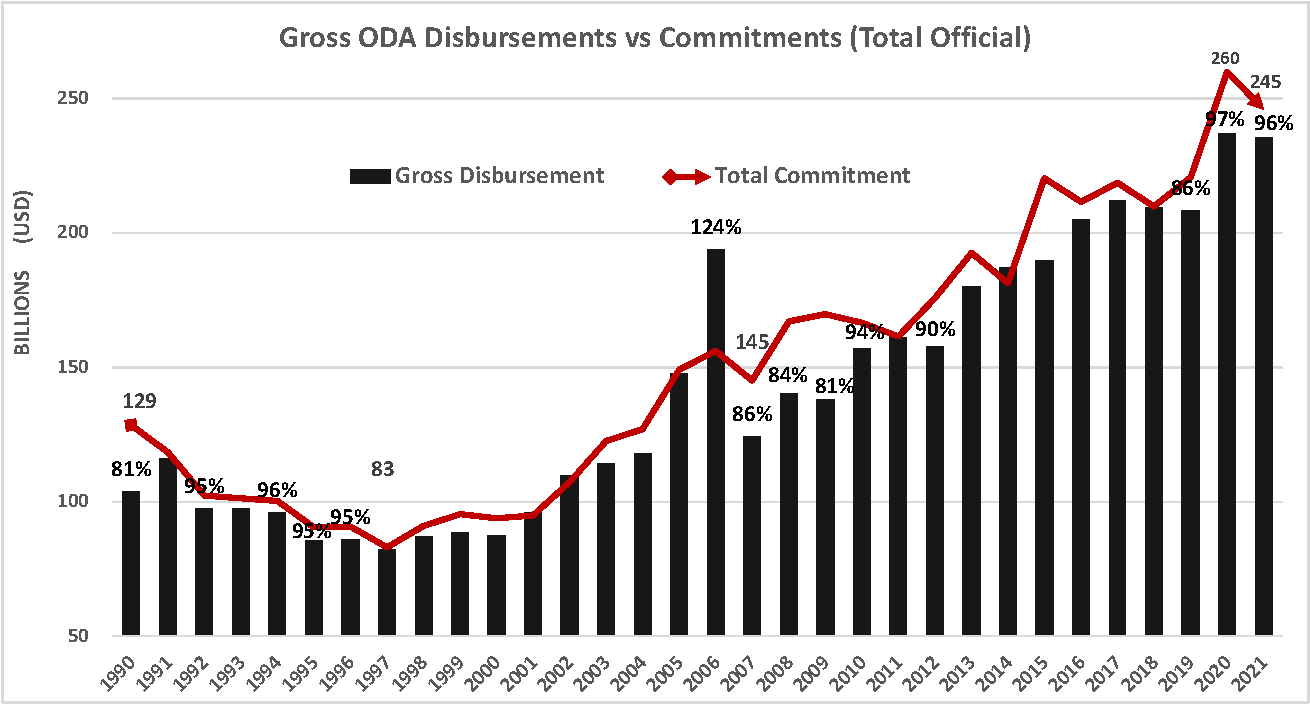
\includegraphics[width = 0.7\textwidth]{Figures/ODA_Graphs/Dibs_VS_Commit.pdf}
    \label{Disbursement Vs Commitment}
\caption*{\footnotesize{Note: Both ODA commitment and disbursement are in 2021 constant price, in USD billion. Author's computation with data from \textcite{oecd_Data_2023}.}}
\end{figure}

%%%%%%%%%%%%%%%%%%%%%%%%%%%%%%%%%%%%%%%%%%%%%%%%%%%%%%%%%%%%%%%%%%%%
% ODA commitment by sectors  						yes
 Figure \ref{fig:ODA sectors commitment} further illustrates the distribution of ODA commitments across sectors.Notably, the social infrastructure and humanitarian sectors emerge as primary recipients of ODA commitments. The Humanitarian sector witnessed substantial growth in committed ODA, escalating from 1\% (1.7 billion USD) of total ODA in 1990 to 16\% in 2021, signifying a remarkable 1,600\% increase over the data period. Simultaneously, the social infrastructure sector rose from 30 billion USD (24\%) in 1990 to a peak of 103 billion USD (43\%) in 2007, subsequently experiencing a gradual reduction to 42\% in 2019. It's crucial to note that while the percentage decreased, the absolute value continued to show an upward trend. This reduction in percentage is attributed to the overall increase in total ODA commitments over the years. The surge in commitments to the humanitarian and social infrastructure sectors since the 2000s can be linked to the MDGs and the subsequent SDGs, reflecting global commitments to addressing poverty and social challenges. Similarly, commitment to economic infrastructures also increased in absolute value starting from 22.5 billion USD or 18\% of the total ODA commitment in 1990 to 35.2 billion or 14\% in 2021. Therefore, considering the pattern of commitments, particularly to the humanitarian and social infrastructure sector, it is logical to consider the total ODA for measuring the effectiveness of ODA.

\begin{figure}[ht]
\captionsetup{justification=justified,singlelinecheck=false}
\caption{\textit{Sectoral ODA Commitments}}
    \centering 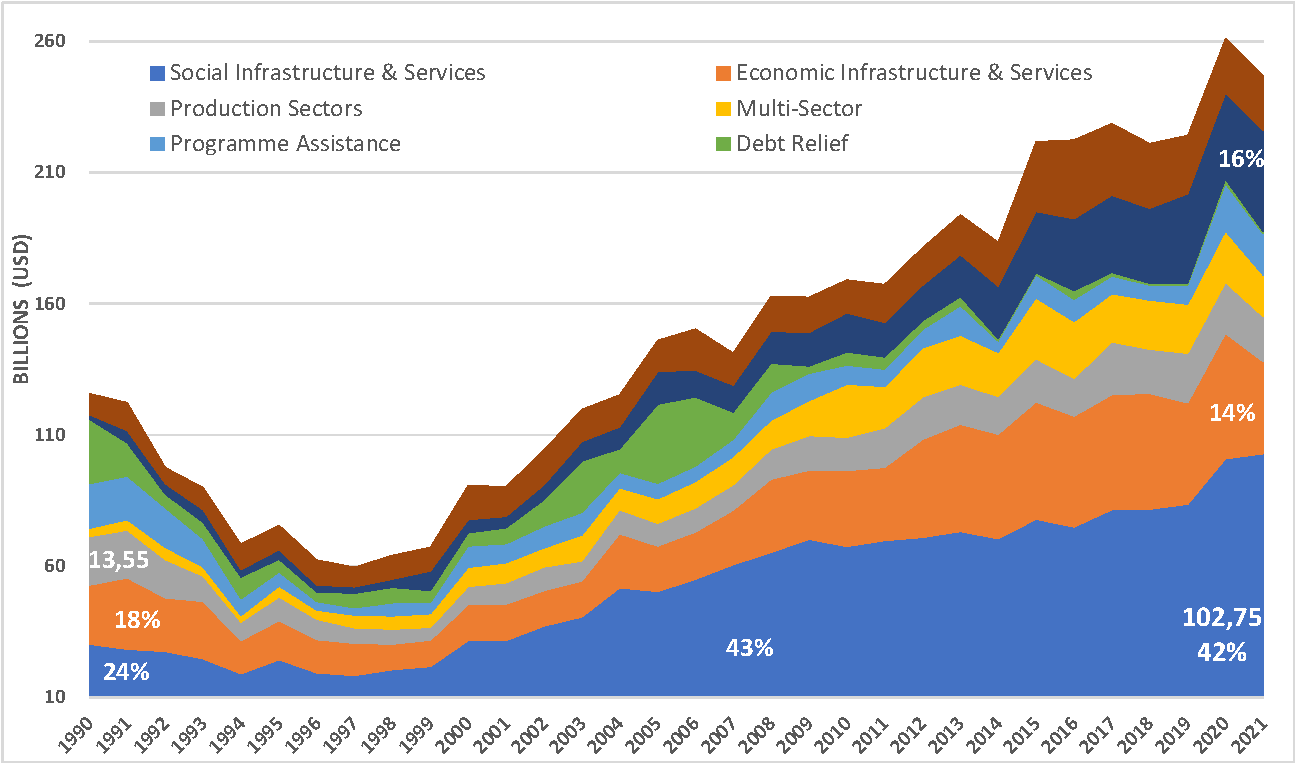
\includegraphics[width = 0.7\textwidth]{Figures/ODA_Graphs/Sector_class.pdf}
    \label{fig:ODA sectors commitment}
    \caption*{\footnotesize{Note. Data for sectoral allocation of ODA is only available for commitment, and not disbursement. However, given the closeness of the two, commitment is a valid proxy for disbursement. Data is in USD billion 2021 constant price, Author's computation with data from \textcite{oecd_Data_2023}}}
\end{figure}

%%%%%%%%%%%%%%%%%%%%%%%%%%%%%%%%%%%%%%%%%%%%%%%%%%%%%%%%%%%%%%%
% Social Infrastructure subsector of ODA 					yes
Particularly crucial to this thesis is the allocation to social infrastructure, which include the health subsector. Figure \ref{fig:Subsector of Social Infrastructure} illustrates the evolving interest and commitment of donors over time in the six subsectors of the social infrastructure sector. Notably, ODA to the health sector grew consistently both in relative and absolute terms, from 13\% in 1990 to 31\% of the total social infrastructure sector by 2021. This growth is most visible in Covid-19 pandemic, with health commitments increasing by over 10\% between 2019 and 2021. The emphasis on health extends to the reproductive health and population subsector, which also experienced substantial growth, rising from 4\% of the total commitment to 12\% in 2021. However, ODA's commitment to water sanitation and education has declined, indicating a shifting pattern in donors' interests over time. Support for government budgets reached its zenith in 2004, constituting 35\% of the total commitment, but has gradually decreased to 22\% by 2021.

\begin{figure}[ht]
\captionsetup{justification=justified,singlelinecheck=false}
\caption{\textit{Evolution of ODA in Social Infrastructure Sector(ODA Commitments)}}
    \centering 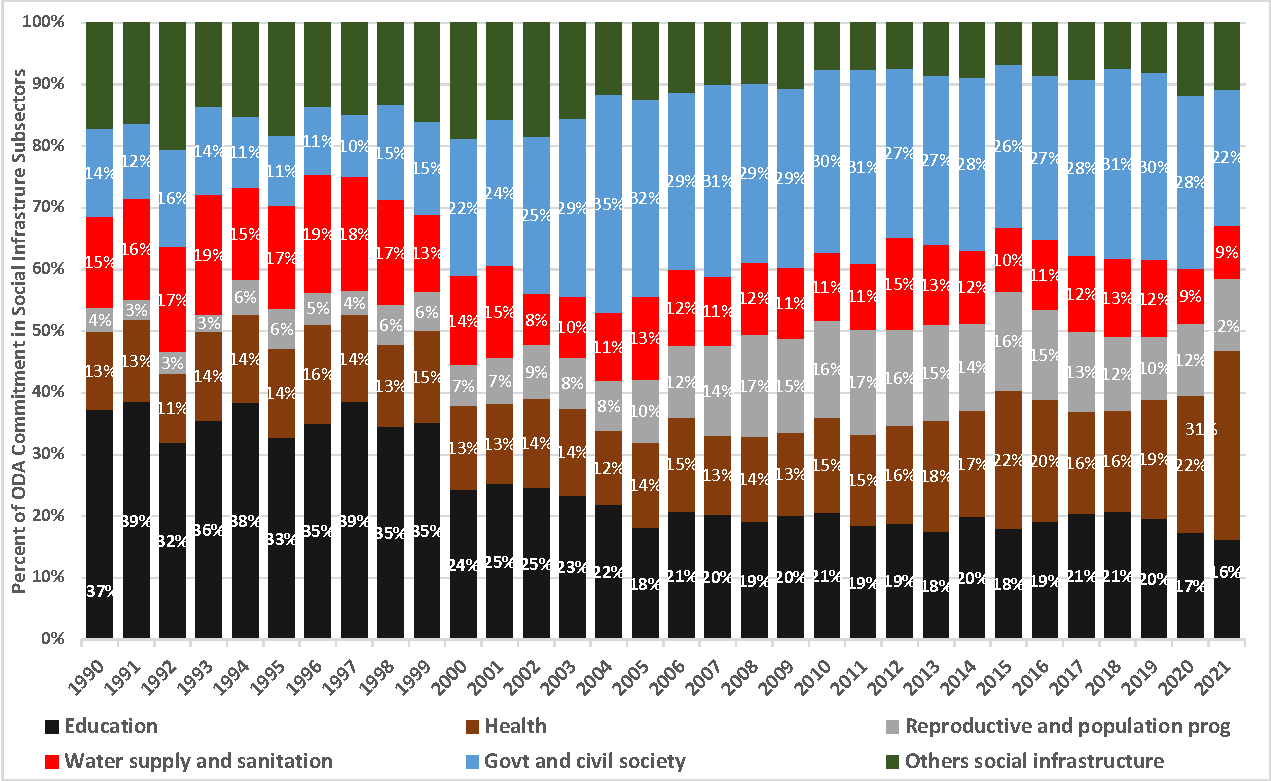
\includegraphics[width = 0.7\textwidth]{Figures/ODA_Graphs/Subsectors_soc_inf.pdf}
    \label{fig:Subsector of Social Infrastructure}
    \caption*{\footnotesize{Despite growth in health ODA, unspecified social infrastructure ODA is high, as shown in Fig \ref{fig:Subsector of Social Infrastructure}. Therefore, the thesis combines the social infrastructure ODA with the total Net ODA for the main analysis. Author's computation with Data from \textcite{oecd_Data_2023}}}
\end{figure}

%%%%%%%%%%%%%%%%%%%%%%%%%%%%%%%%%%%%%%%%%%%%%%%%%%%%%%%%%%%%%%%%%%%%%%%%%%
\paragraph{\quad \quad \textit{2.1.2.2  ODA Characterization by Donors}}
% DAC donors and non-dac donors   Evolution of Net ODA disbursement yes 
\paragraph{}Figure \ref{fig:ODA by donors} illustrates the distribution of ODA donors, categorizing them into DAC (Development Assistance Committee) donors, which are OECD member countries providing bilateral ODA to developing nations, and non-DAC bilateral and multilateral net ODA donors. DAC countries consistently play a significant role as ODA donors, contributing around 67\% of the total ODA. This percentage was equivalent to 61.4 billion in 1990 and increased to 63\% or 129.3 billion in 2021. While the DAC bilateral ODA declined in 2014, it still constituted a substantial portion, accounting for 67\% or 92 billion of the total. Multilateral donors constituted 20\% of ODA in 1990, growing to 28\% or 57.4 billion in 2021. In contrast, non-DAC ODA had a relatively negligible share, ranging from 10\% in 1990 to fluctuating between 2\% and 5\% during the 2000s. Notably, there has been significant growth in non-DAC countries' ODA since 2010, reaching 9\% or 19.36 billion.

\begin{figure}[ht]
\captionsetup{justification=justified,singlelinecheck=false}
\caption{\textit{Evolution of Net ODA Disbursement by Donors}}
    \centering 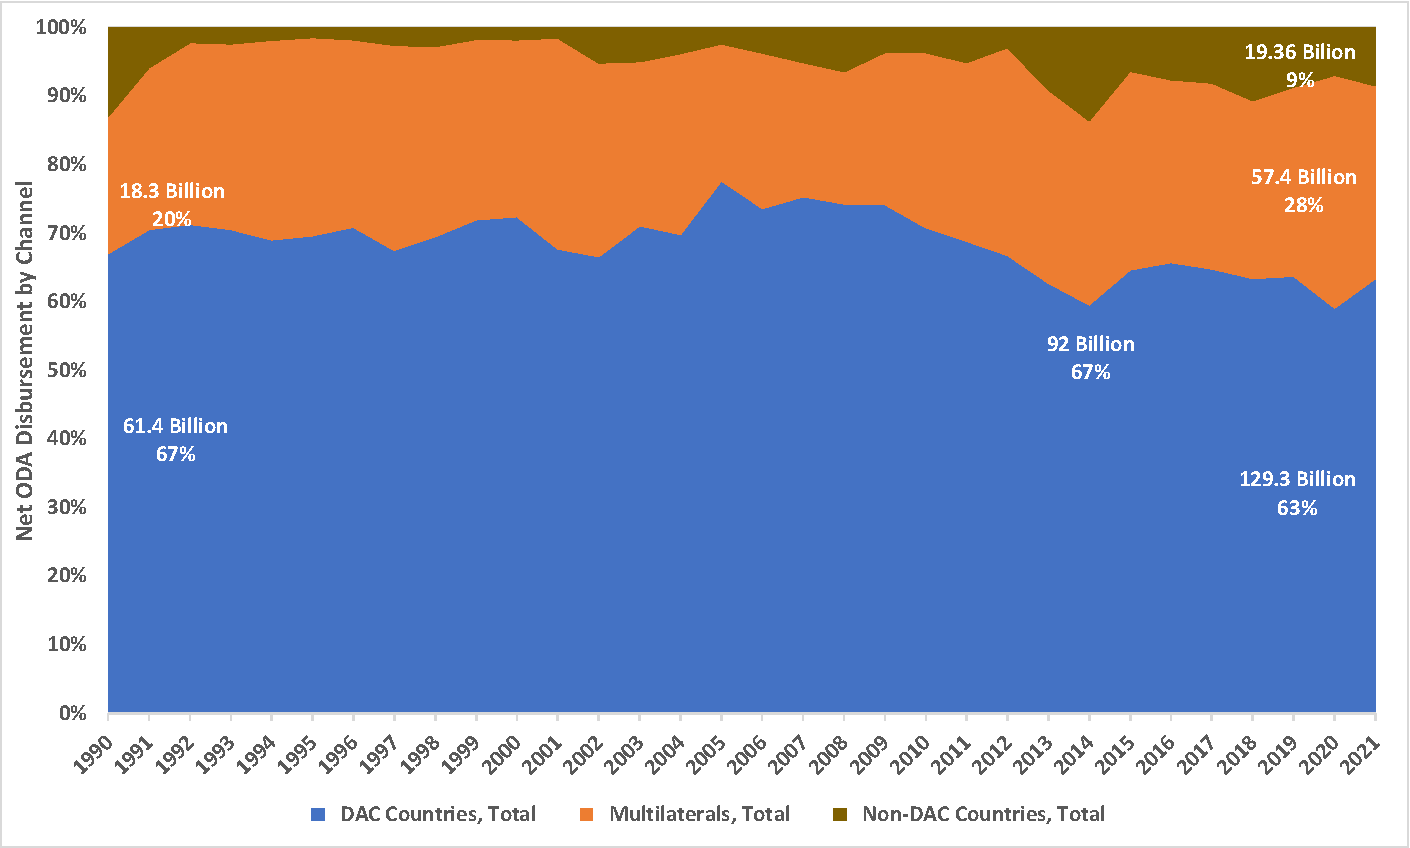
\includegraphics[width = 0.7\textwidth]{Figures/ODA_Graphs/Evolution_Net_ODA.pdf}
    \caption*{\footnotesize{Note. Percentage is the author's computation using Net ODA in 2021 constant price, data from \textcite{oecd_Data_2023}}}
    \label{fig:ODA by donors}
\end{figure}

%%%%%%%%%%%%%%%%%%%%%%%%%%%%%%%%%%%%%%%%%%%%%%%%%%%%%%%%%%%%%%%%%%%%%%%%%%%%%%H%ighest Net ODA Donors among DAC 			yes

In Figure \ref{fig:Highest ODA donors}, among the DAC donors, the United States (US) has consistently been the highest donor since 1990, allocating 25\% or 15 billion USD of the total DAC ODA. The US experienced a significant decline in ODA in 1996, impacting the global ODA allocation. Despite being a major donor, the US reached a record low of 7.9 billion or 17\% during the early 1990s recession. Subsequently, US ODA steadily increased, reaching 34 billion or 34\% of DAC's total ODA before declining again due to the 2008 recession. Germany, on the other hand, initially the fourth-highest DAC donor with 7 billion or 12\% of the total DAC in 1990, ascended to the second-highest donor in 2006, surpassing France and Japan. By 2016, Germany disbursed approximately 20\% or 23 billion of the total DAC. France and Japan's ODA remained relatively stable, fluctuating between 13\% and 14\% of the total DAC in 1990 to 8\% and 9\% in 2021. Notably, Germany's ODA exhibited relative stability and predictability over the years, with fewer cyclical changes compared to the USA.

\begin{figure}[ht]
\captionsetup{justification=justified,singlelinecheck=false}
\caption{\textit{Highest Donors of Net ODA Disbursement in DAC Countries}}
\vspace{4pt}
    \centering 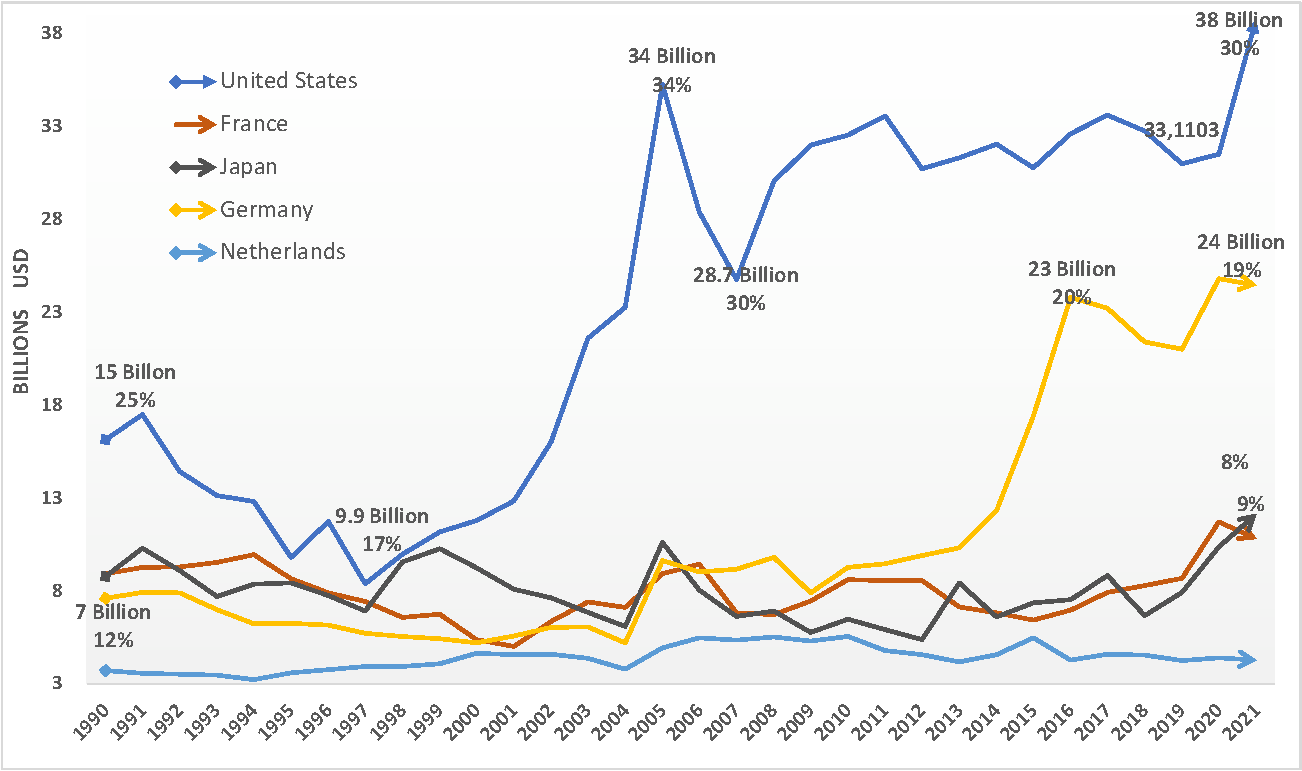
\includegraphics[width = 0.7\textwidth]{Figures/ODA_Graphs/Top_DAC_Donors.pdf}
    \caption*{\footnotesize{Net ODA in 2021 constant price billion USD. Author's computation with sata from \textcite{oecd_Data_2023}}}
    \label{fig:Highest ODA donors}
\end{figure}

%%%%%%%%%%%%%%%%%%%%%%%%%%%%%%%%%%%%%%%%%%%%%%%%%%%%%%%%%%%%%%%%%%
\paragraph{\quad \quad \textit{2.1.2.3 ODA Characterization by Recipients}}
% Time and regional distribution of Net ODA by continents    yes
\paragraph{} Figure \ref{fig:ODA by continent} presents the distribution of ODA recipients by continents. Accordingly, the African continent has consistently been the highest recipient of Net ODA, with the estimated amount increasing from 42 billion USD or 46\% of the total ODA in 1990 to 75 billion or 37\% in 2021. Asia follows, with the amount growing from 26 billion or 29\% in 1990 to 54 billion or 26\% in 2021. Although both Africa and Asia's ODA grew relatively close, with an increase of 28 billion over 30 years, Africa's ODA reduced in relative terms compared to Asia.

\begin{figure}[ht]
\captionsetup{justification=justified,singlelinecheck=false}
\caption{\textit{Recipients of ODA by Continents}}
\vspace{4pt}
    \centering 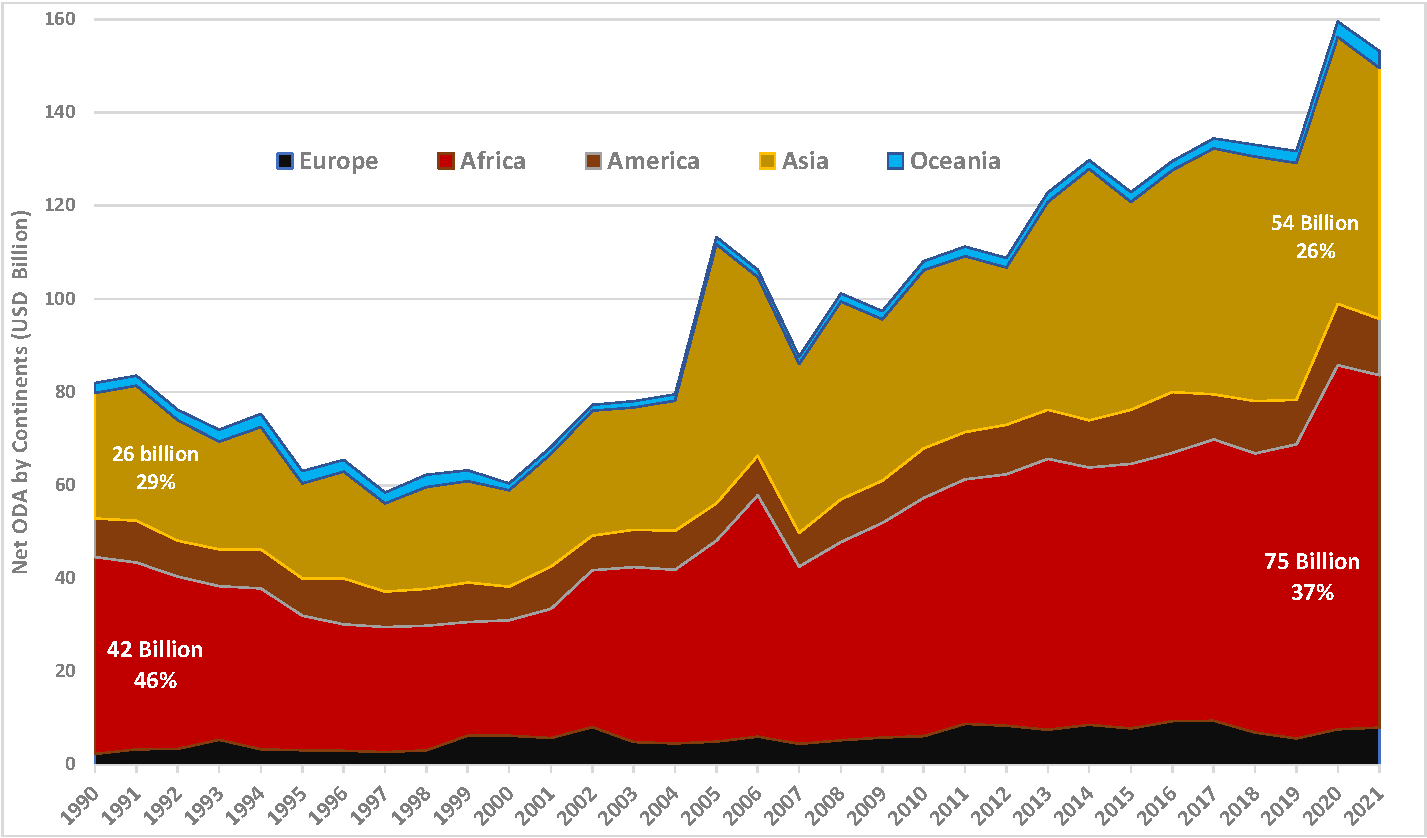
\includegraphics[width = 0.7\textwidth]{Figures/ODA_Graphs/Dist_ODA_by_continents.pdf}
    \caption*{\footnotesize{Note: Net ODA in 2021 constant price billion USD. Author's computation, with data from \textcite{oecd_Data_2023}}}
    \label{fig:ODA by continent}
\end{figure}


However, a more detailed examination at the country level, as depicted in Appendix Figure \ref{fig:ODA highest recipient}, reveals a nuanced scenario. Only three African and seven Asian countries are among the top ten recipients of Net ODA. Iraq leads as the highest net ODA recipient, averaging 3.2 billion USD, closely followed by Afghanistan with 3.1 billion. Notably, conflict-affected countries such as Iraq, Afghanistan, Congo DRC, and Ethiopia account for a significant volume of ODA. Additionally, India ranks as the seventh-highest net ODA recipient, followed by Bangladesh and Tanzania.





%ODA dependency \footnote{ODA dependency defined as the percentage of Net ODA received per recipient GNI.}, as used in other studies \textcite{temple_aid_2010}, provides a magnified view of the aid landscape across countries and regions. This is illustrated in Figure \ref{fig:ODA Dependency by region} and Appendix Figure \ref{fig:aid dependency}. Accordingly, all the regions are statistically different in their level of aid dependency. These figures reveal that Sub-Saharan Africa (SSA) is the highest aid-dependent region, notable highly aid-dependent countries in SSA include Ethiopia, Mozambique, Rwanda, Liberia, and the Central African Republic, as shown in Appendix Figure \ref{fig:aid dependency}.



\begin{figure}[ht]
\captionsetup{justification=justified,singlelinecheck=false}
\caption{\textit{Regional Comparison of Aid Dependency: ODA per Countries' GNI}}
    \centering 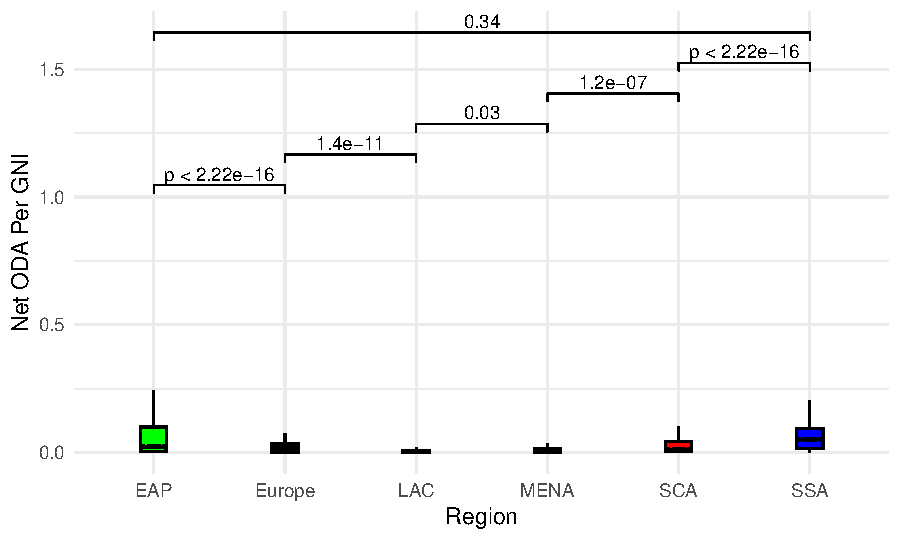
\includegraphics[width = 0.7\textwidth]{Figures/ODA_Graphs/ODA_GNI_boxplt.pdf}
    \caption*{\footnotesize{Note: ODA is logged to reduce outliers. The P-values are derived from the t-test, for statistical differences among the regions. Author's compuataion with data from \textcite{oecd_Data_2023}}}
    \label{fig:ODA Dependency by region}
\end{figure}

ODA dependency, defined as the percentage of Net ODA received per recipient GNI, provides a nuanced view of the aid landscape across countries and regions, as used in other studies \textcite{temple_aid_2010}. This is highlighted in Figure \ref{fig:ODA Dependency by region} and Appendix Figure \ref{fig:aid dependency}. All regions show statistically significant differences in their levels of aid dependency. Sub-Saharan Africa (SSA) emerges as the highest aid-dependent region, particularly in countries such as Ethiopia, Mozambique, Rwanda, Liberia, and the Central African Republic, as depicted in Appendix Figure \ref{fig:aid dependency}. Similarly, the South and Central Asia (SCA) and East Asia and Pacific (EAP) regions exhibit high and comparable levels of aid dependency, influenced particularly by small countries such as Marshall Islands and Tuvalu. Despite the relatively low incidence of ODA dependency in the Middle East and North Africa (MENA) region, war-torn countries like Iraq and Syria demonstrate extreme values of dependency on a global scale.



%%%%%%%%%%%%%%%%%%%%%%%%%%%%%%%%%%%%%%%%%%%%%%%%%%%%%%%%%%%%%%%%%%%%%%%%%%%%%%%%%%%%%%%%%%%%%%%%%%%%%%%%%%%%%
\subsection*{2.2 Health Outcome}
\addcontentsline{toc}{subsection}{2.2 Health Outcomes}
\subsubsection*{\quad 2.2.1 Conceptualizing Health Outcomes}
\addcontentsline{toc}{subsubsection}{2.2.1 Conceptualizing Health Outcomes}

\paragraph{}The term "health outcome" encapsulates two constructs: "outcome" and "health." Both Oxford and Cambridge dictionaries define an outcome as a consequence, a result or effect of an action or event \parencite{cambridge_dictionary_outcome_2023, oxford_dictionary_outcome_nodate}. Thus, an outcome could be semantically attributed to the consequence of an action(s) in any context by any capable being. The concept of “health”, on the other hand, is pluralistic and has evolved. Historically, health was perceived in terms of physiological functioning: a harmony between the human mind and social environment \parencite{svalastog_concepts_2017}. 

A more holistic view, conceptualized within the bio-psychosocial framework, is reflected in the WHO 1948 constitution. According to it, health is defined as "the state of complete physical, mental, and social well-being and not merely the absence of disease or infirmity" \parencite{who_constitution_1946}. This definition underscores social welfare as a crucial component of human health, acknowledging the impact of living and working conditions on health \parencite{svalastog_concepts_2017}. A notable linkage between health and economic conditions is traceable to the health production theory, which emphasizes the relevance of health capital to economic capacity \parencite{grossman_concept_1972}. Reflecting on the capability perspective with the temporal dynamics of health, \textcite{huber_how_2011} define health as the ability to adapt and self-management, particularly to handle social, physical and emotional problems. Also, nutrition has become an essential aspect of health over time \parencite{gamble_why_2008} \footnote{According to the Food and Agriculture Organization (FAO), nutrition interacts with health in three important ways: increased body demand for nutrition to maintain homeostasis; reduction of food intake; and waste from vomiting \parencite{fao_study_1996}}. 

Therefore, the thesis draws insight from Shafa and colleagues' \parencite{shafa_assessment_2023} definition of health outcomes. Accordingly, health outcome is defined as tool(s) for assessing the impact of care or intervention on people's health situation. Since health is multidimensional, health metrics are equally complex. Health outcome metrics may be include indicators such as life expectancy, child mortality, and morbidity \parencite{shafa_assessment_2023} as well as composite indices i.e. Universal Health Coverage (UHC) index. SDG 3, focusing on health and well-being provides international indicators critical for assessing health outcomes and crucial for this study. The six composite health dimensions are discussed below. 
% Another uniqueness of this thesis is the incorporation of nutrition to measure health outcomes, accommodating regional differentials in the burden of health. This section further explores the distribution of crucial health outcome indicators across countries and regions.

%%%%%%%%%%%%%%%%%%%%%%%%%%%%%%%%%%%%%%%%%%%%%%%%%%%%%%%%%%%%%%%%%%%%%%%%
\subsubsection*{\quad 2.2.2 Characterizing Health Outcomes in Developing Countries}
\addcontentsline{toc}{subsubsection}{2.2.2 Statistical Characterization of Health Dimensions}
This thesis employs a comprehensive approach to measure health outcomes by considering the multidimensionality of health. It incorporates 25 unique indicators from SDG 2 and 3 for health and malnutrition, respectively. These indicators are employed to create six composite health dimensions: Reproductive Fatality and Teen Pregnancy (RFTP), Burden of Infection and Diseases (BID), Burden of Mental Problems (BMP), Malnutrition, Environmental Death, and Health System Capacity and Responsiveness (HSCR). All unique indicators are standardized to ensure comparability (see the procedure in Appendix B.1). Figure \ref{fig:combined_Box_plot} displays the six health dimensions, with each panel representing one dimension. The associated p-values, derived from t-tests, determine the significant differences in health dimensions among regions, to justify inaccuracy of using narrow health indicators to assess ODA effectiveness.


%\caption*{\footnotesize{Note: Each panel of the graph represents each of the six composite health dimensions, created using equal weightings. Plot A contains Reproductive fatality and Teen Pregnancy (RFTP), Plot B shows Burden of Infection and diseases (BID). Plot C illustrates the Burden of Mental Problems (BMP). Plot D represents Malnutrition, Plot E on Environmental Death and Plot F for Health System Capacity and Responsiveness (HSCR). See respective indicators for various health dimensions in Appendix Table \ref{Tab::health indicators}. Lines in the middle of boxes indicate the median, the bottom and top of each box are the 25th and 75th quartile respectively, while whiskers represent the 95\% Confidence Interval (CI). The kernel density curve indicates the distribution of specific health dimensions within respective regions. Author's computation, data from \textcite{unsdg_sustainable_2023, wdi_world_2023}}}
 
Starting from RFTP, in Figure \ref{fig:combined_Box_plot} Plot A, all regions are significantly different. SSA region has the highest RFTP, densely distributed among its countries, with specific countries such as Guinea-Bissau, Sierra Leone, Chad, Liberia, Rwanda, and Nigeria ranking among the worst (see Appendix B.2 Figure \ref{fig:combined_scat_plot} for country-level details). SCA also shows moderately high RFTP, but many countries within the region are below its median. Europe, on the other hand, has the lowest reproductive fatalities (RFTP), with most countries clustered around its median. In Plot B of Figure \ref{fig:combined_Box_plot}, infection and disease (BID) also significantly vary across the regions. Notably, both SSA and SCA have the worst BID cases, densely distributed among their countries. India, Kiribati, Lesotho, Swaziland, Zimbabwe, Ethiopia, and the Central African Republic (CAF) have the highest BID, as shown in Appendix B.2 Figure \ref{fig:combined_scat_plot}.


\begin{landscape}
    \begin{figure}[ht]
\captionsetup{justification=justified,singlelinecheck=false}
\caption{\textit{Composite Health Dimensions Across Regions of Developing Countries}}
    \centering 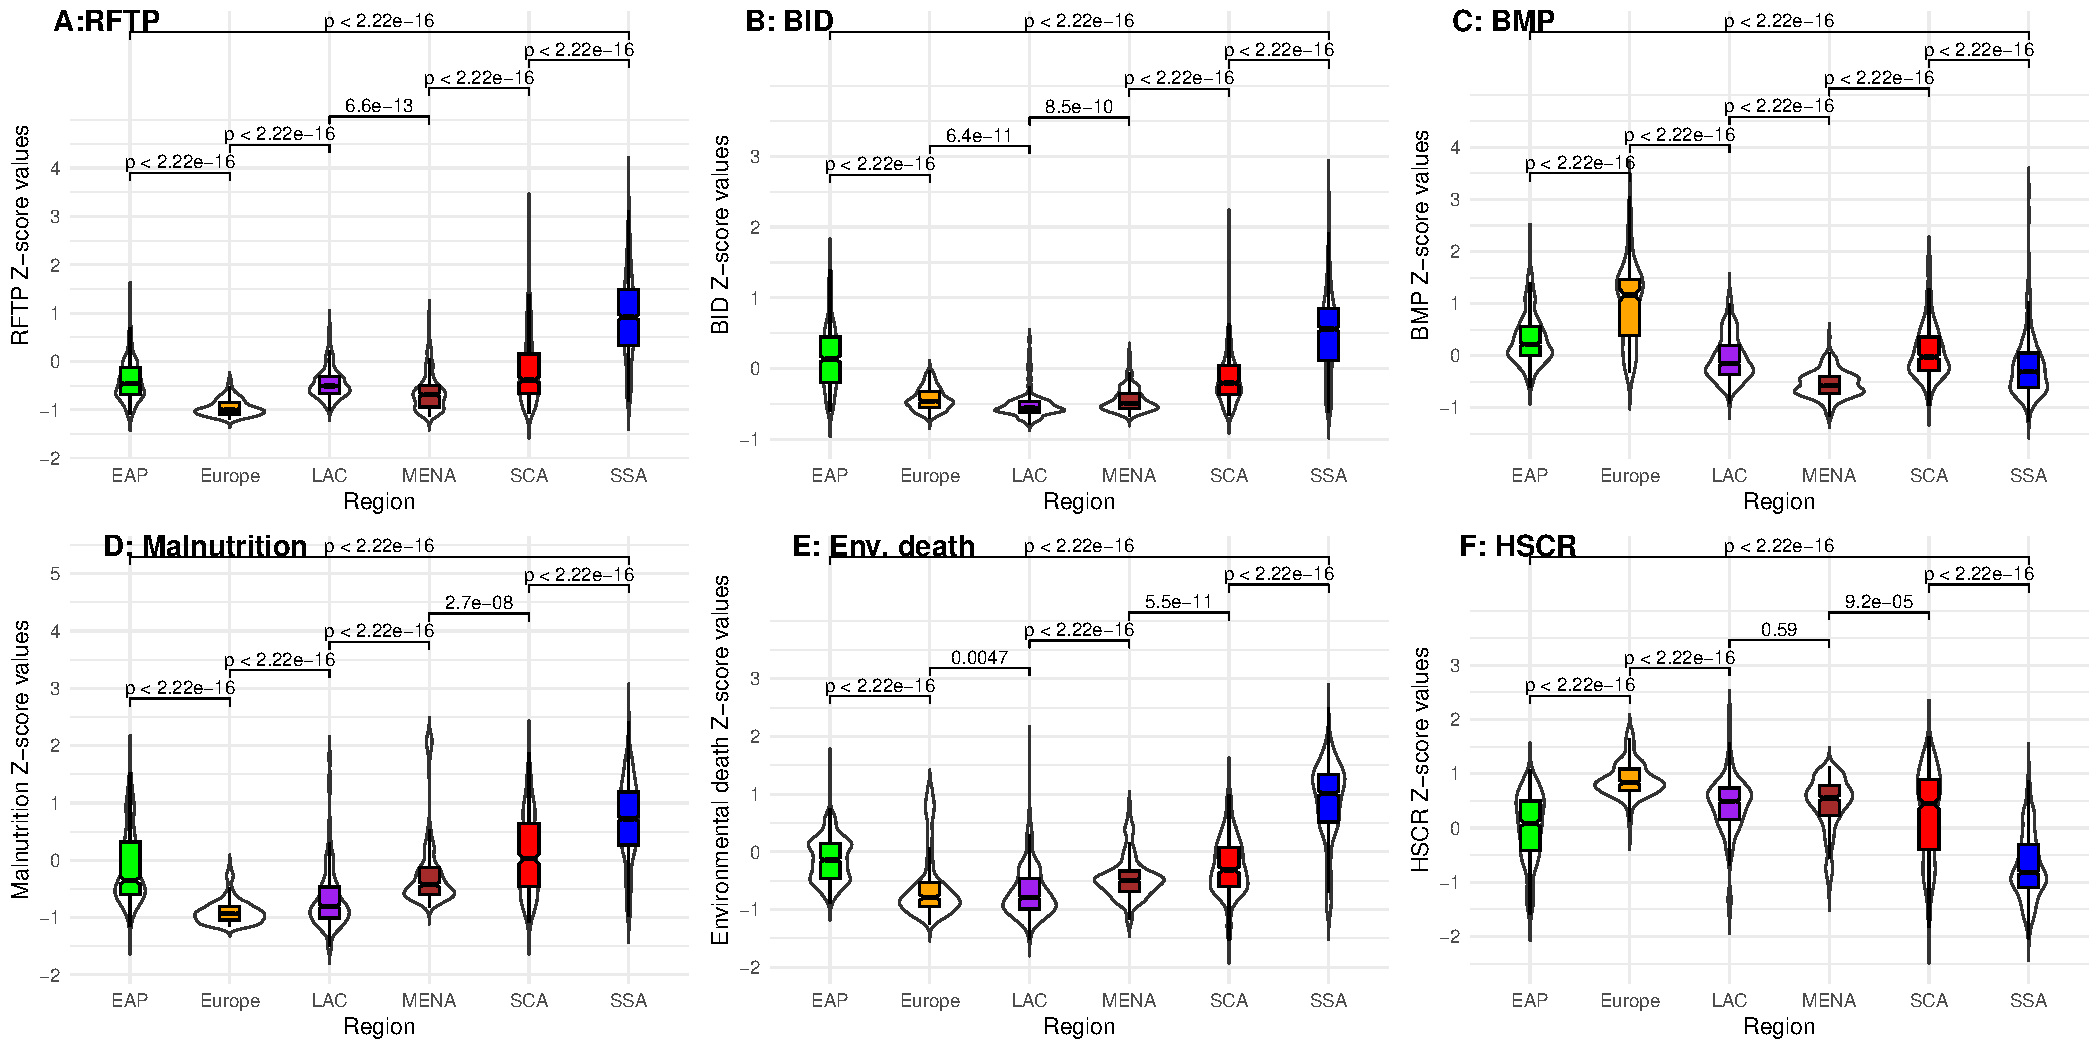
\includegraphics[width = 1.65\textwidth]{Figures/Health_Outcome_Graph/Combined_Boxplt_2.pdf}
    \caption*{\footnotesize{Note: Each panel in the graph corresponds to one of the six composite health dimensions, created with equal weightings. Plot A features Reproductive Fatality and Teen Pregnancy (RFTP), Plot B depicts the Burden of Infection and Diseases (BID), Plot C illustrates the Burden of Mental Problems (BMP), Plot D represents Malnutrition, Plot E focuses on Environmental Death, and Plot F addresses Health System Capacity and Responsiveness (HSCR). See specific health indicators for each health dimension in Appendix Table \ref{Tab::health indicators}) and procedure in Appendix B.1. Author's computation, data sourced from \textcite{unsdg_sustainable_2023, wdi_world_2023}.}}
    \label{fig:combined_Box_plot}
\end{figure}
\end{landscape}


Mental problem, depicted in Figure \ref{fig:combined_Box_plot} Plot C as Burden of Mental Health (BMP), is highest in Europe and widely dense among its countries. Specific European countries with the highest incidence include Ukraine, Belarus, Serbia, and Croatia. BMP shows significant differences across all regions, with MENA and SSA having the lowest cases, and most countries in these regions falling below their respective regional median value. For the malnutrition health dimension (Plot D in Figure \ref{fig:combined_Box_plot}), all regions exhibit statistically significant differences, with the highest cases in SSA, SCA, and EAP. SSA has the highest malnutrition, densely distributed among its countries. While SCA and EAP also show high malnutrition, the situation tends to be more spread in SCA countries than in EAP.

Environmental death, presented in Figure \ref{fig:combined_Box_plot} Plot E, significantly varies across regions, with the highest in SSA. SCA and EAP also exhibit very high environmental death, but with different distribution patterns. SCA countries have a high density below the region's median, while most EAP countries are above their region's median value. Finally, Health System Capacity and Responsiveness (HSCR) in Figure \ref{fig:combined_Box_plot} Plot F show significant differences across regions, except between LAC and MENA regions. Europe has the highest HSCR, with most countries clustering in the 75th quartile of its region. While both LAC and MENA regions also have high health capacity, SSA stands out with the poorest health system among the regions compared.




%Considering the multidimensionality of health, this thesis adopts a comprehensive approach to measuring health outcomes, incorporating 25 unique indicators from SDG 2 and 3 for health and malnutition, respectively. All indicators are used to create six composite health dimensions: Reproductive Fatality and Teen Pregnancy (RFTP), Burden of Infection and Diseases (BID), Burden of Mental Problem (BMP), Malnutrition, environmental death, and Health System Capacity and Responsiveness (HSCR). Specific indicators within each dimension are standardized before creating dimension indices to ensure comparability (see procedure in Appendix B.1). The six health dimensions are presented in Figure \ref{fig:combined_Box_plot}, with each panel representing each health dimension. The p-values are derived from t-test showing whether specific health dimensions is significantly different among regions. This is essential to invalidate the use of narrow health indicators in assessing ODA effectiveness. 


%As shown in Figure \ref{fig:combined_Box_plot} Plot A, RFTP p-value is statistically different across the regions. Specifically, Sub-Saharan Africa (SSA) has the highest RFTP and densely distributed among its countries, with specific countries like Guinea-Bissau, Sierra Leone, Chad, Liberia, Rwanda, and Nigeria ranking among the worst (see Appendix B.2 Figure \ref{fig:combined_scat_plot} for country level). While RFTP is also moderately high in South and Central Asian (SCA) region, many countries are below the region median value. Europe has the lowest reproductive fatalities, with most countries clustered around the median index value, as indicated by the bulge density. In the same Figure \ref{fig:combined_Box_plot} plot B illustrate between region comparison of BID. Accordingly, all regions are statically different in their burden of infections and diseases, value of all sample comparison \textless 1\%. Furthermore, despite regions being closely related on this dimension, both SSA and SCA have the worst BID cases, and densely among their countries, with India, Kiribati, Lesotho, Swaziland, Zimbabwe, Ethiopia, and the Central African Republic (CAF) having the highest, as shown in Appendix B.2 Figure \ref{fig:combined_scat_plot}. 


 %Mental health is equally an essential aspect of human health. Unlike reproductive fatality (RFTP) and infection and diseases (BID) health dimensions, Figure \ref{fig:combined_Box_plot} plot C shows Burden of Mental Health (BMP) is the highest in Europe and, widely dense among its countries. In Appendix Appendix Figure B.2 Figure \ref{fig:combined_scat_plot}, Specific European countries with the highest incidence include Ukraine, Belarus, Serbia, and Croatia. Furthermore, BMP is significantly different across all regions, with Middle East and North Africa (MENA) and SSA having lowest cases, with most countries in the regions below the median value of their respective regional median values. In the malnutrition health dimension, Figure \ref{fig:combined_Box_plot} plot D, all the regions are statistically different, with the highest cases in SSA, SCA and EAP. Specifically, malnutrition is the highest in SSA, and densely distributed among its countries. Malnutrition is also high for SCA and EAP regions, however,  the situation tend to more spread in SCA countries than EAP.


%Environmental death, in Figure \ref{fig:combined_Box_plot} plot E, also significantly vary across, albeit, the level of significance vary. As illustrated in plot E, environmental death is the highest in SSA and the distribution reflects other health dimensions. Both SCA and EAP equally exhibit very high environmental death, but SCA countries have a high density below the region's median, while most EAP countries are above their region's median value. Regardless of the intensity of health problems, health system capacity and responsiveness (HSCR) is essential to handle health problems when arise. As shown in Figure \ref{fig:combined_Box_plot} plot F, HSCR is significantly different across regions with p-value \textless{} 1\% except between LAC and MENA regions. Europe has the highest HSCR, with most of its countries clustering in the 75th quartile of its region. While both LAC and the MENA regions are also high in health capacity, with similar similar distribution shapes among their respective countries, SSA has the poorest health system among the regions compared. 




%\begin{figure}[ht]
%\captionsetup{justification=justified,singlelinecheck=false}
%\caption{\textit{Reproductive Health Risk and Mortality Dimension}}
%    \centering 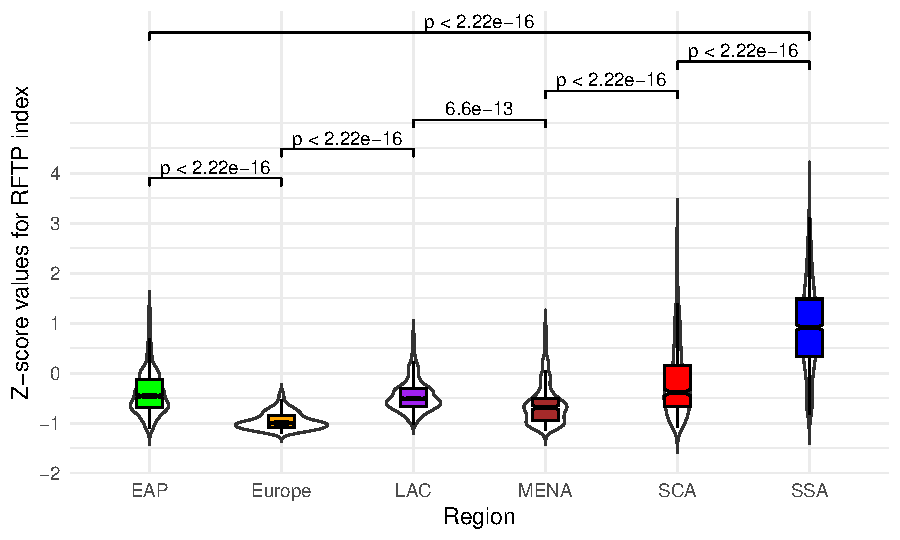
\includegraphics[width = 0.8\textwidth, height = 7cm]{Figures/Health_Outcome_Graph/Reprod_Risks_boxplt.pdf}
 %   \caption*{\footnotesize{Note. Reproductive health risk and mortality index comprises four indicators: maternal, under-5 child and neonatal mortality, and adolescent pregnancy incidence (10 to 19 years) access across the regions of interest. Author's computation, data from \textcite{unsdg_sustainable_2023, wdi_world_2023}}}
  %  \label{fig:reproduction boxplot}
%\end{figure}


%1.65


%

% Figure: Burden of Infection and diseases 


% Figure: Mental Health Problem

%\begin{figure}[ht]
%\captionsetup{justification=justified,singlelinecheck=false}
%\caption{\textit{Mental Health Dimension}}
 %   \centering 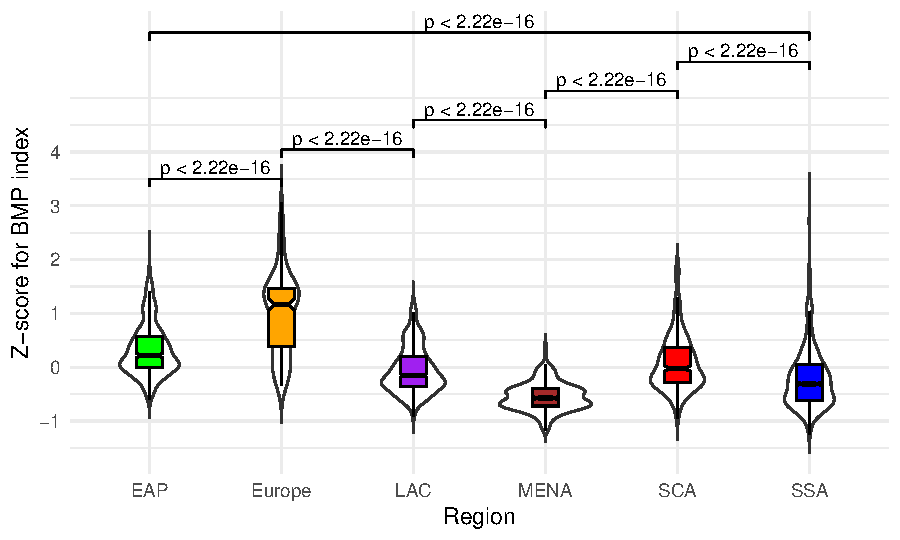
\includegraphics[width = 0.8\textwidth, height = 7cm]{Figures/Health_Outcome_Graph/Mental_Hth_boxplt.pdf}
  %  \label{fig:Mental health}
   % \caption*{\footnotesize{Note. Mental health dimension is derived from three indicators: mortality by suicide, alcohol per capita consumption, and population incidence of tobacco. P-value derived from two-way paired t-test. All regions are significantly different at p-value \textless{} 1\%. Author's computation, data from \textcite{unsdg_sustainable_2023, wdi_world_2023}}}
%\end{figure}


%\begin{figure}[ht]
%\captionsetup{justification=justified,singlelinecheck=false}
%\caption{\textit{Burden of Infection and Diseases Dimension}}
 %   \centering 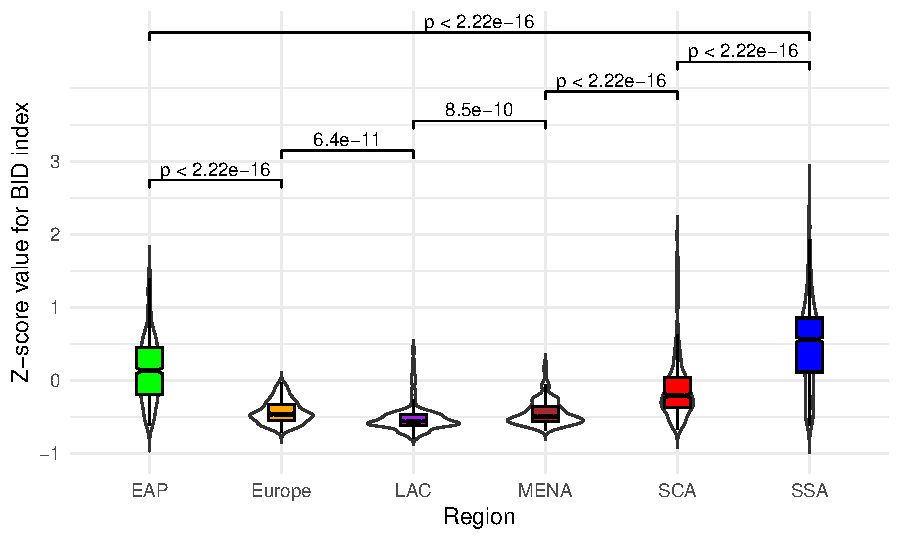
\includegraphics[width = 0.8\textwidth, height = 6cm]{Figures/Health_Outcome_Graph/Burd_Infs_boxplt.pdf}
  %  \label{fig:Infection burden}
   % \caption*{\footnotesize{Note. The burden of infection and diseases (BID) five indicators: new HIV cases, population tuberculosis incidence, malaria incidence, hepatitis-B among under-5, tropical diseases and mortality rate from non-communicable diseases \footnote{Example of Non-communicable disease (NDC) are cardiovascular disease, cancer, diabetes or chronic respiratory disease}.  P-value derived from two-way paired t-test. All regions are significantly different at p-value \textless{} 1\%. Author's computation, data from \textcite{unsdg_sustainable_2023, wdi_world_2023}}}
%\end{figure}



% Figure: Incidence of Malnutrition
%In malnutrition dimension, Figure \ref{fig:malnutrition index}, all the regions have statistically different levels of malnutrition. Specifically, SSA has the highest malnutrition intensity among all the regions, with most countries in the region below its regional 75th quartile. Malnutrition intensity is also high for SCA and EAP regions, however, the density distribution varies across the two. While malnutrition intensity is widely spread in SCA countries, most EAP countries are below its regional median value. Both the LAC and the MENA regions exhibit moderate malnutrition, while Europe has the lowest intensity (see Appendix 6 for country comparison).
%\begin{figure}[ht]
%\captionsetup{justification=justified,singlelinecheck=false}
%\caption{\textit{Dimension Index for Malnutrition}}
 %   \centering 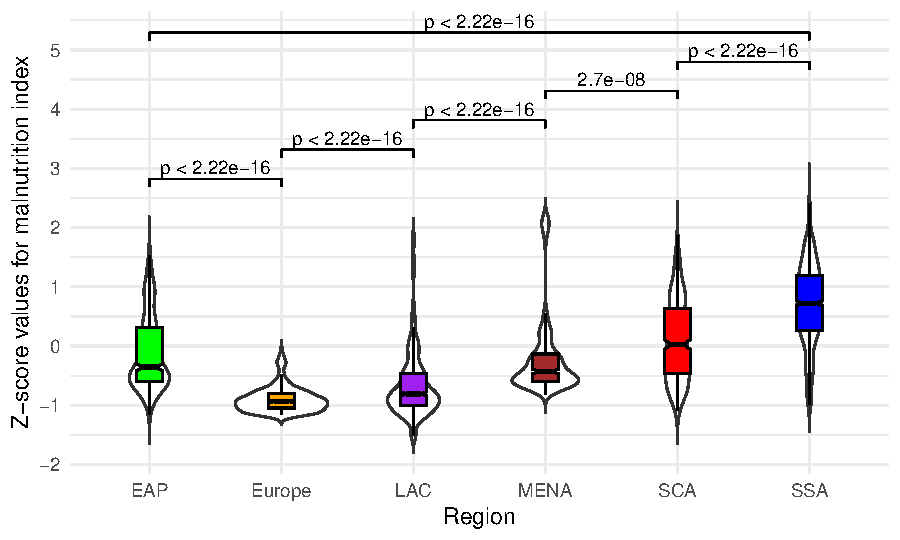
\includegraphics[width = 0.8\textwidth, height = 7cm]{Figures/Health_Outcome_Graph/Malnutrition_boxplt.pdf}
  %  \label{fig:malnutrition index}
   % \caption*{\footnotesize{Note. Malnutrition dimension comprises three indicators specifically from SDG 2: Percentage of 15 - 49 years women with anemia, population undernutrition, and under-5 children moderately or severely stunted. Author's computation, data from \textcite{unsdg_sustainable_2023, wdi_world_2023}.}}
%\end{figure}
% Figure: Environmental Induce Death
%Unlike previous health dimensions, not all regions are statistically different in environmental death. As illustrated in Figure \ref{fig:Env mortality}, while other regions are statistically different (p-value \textless{} 5\%), Europe and Latin America (LAC) are similar in environmental death (p-value \textgreater{} 5\%). Specifically,  SSA has the highest environmental death and is statistically different from all other regions. However, most of its countries experience environmental mortality above the region's median value. Both SCA and EAP equally exhibit very high environmental mortality, but the distribution among countries differs between the two regions. SCA countries have a high density below the region's median, while most EAP countries are above their region's median value. Environmental mortality density is similar across Europe, LAC, and MENA regions.

%\begin{figure}[ht]
%\captionsetup{justification=justified,singlelinecheck=false}
%\caption{\textit{Dimension Index for Environmental Related Mortality}}
 %   \centering 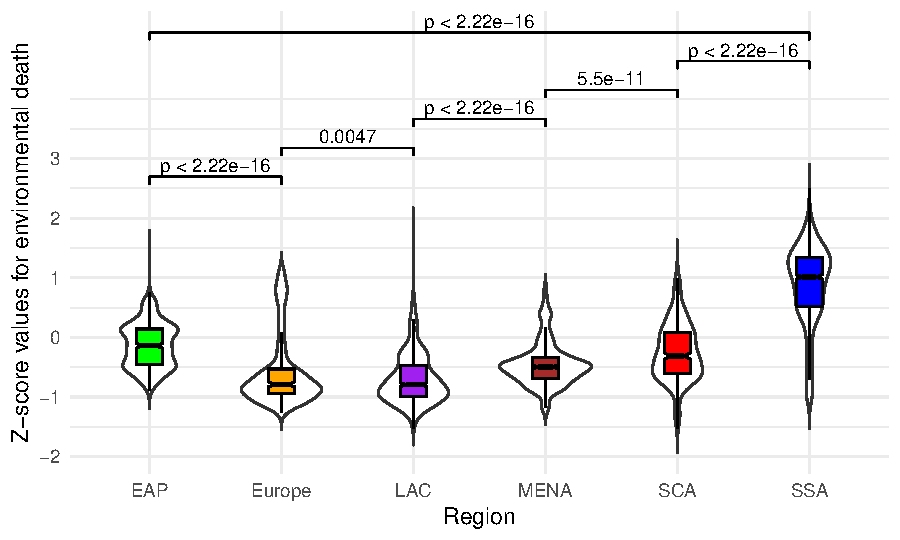
\includegraphics[width = 0.8\textwidth, height = 7cm]{Figures/Health_Outcome_Graph/Env_death_boxplt.pdf}
  %  \label{fig:Env mortality}
   % \caption*{\footnotesize{Note. Environmental mortality, as a dimension, comprises four mortality-based indicators: air pollution, unintentional poisoning, unclean water, and road traffic mortality. P-value derived from two-way paired t-test. All regions, except Europe and LAC, are significantly different. Author's computation, data from \textcite{unsdg_sustainable_2023, wdi_world_2023}}}
%\end{figure}




% Figure: Health System Capacity and Responsiveness
%Regardless of the intensity of health problems, health system capacity and responsiveness is essential to handle health problems when arise. Figure \ref{fig:Health syst Cap} shows all regions are statistically different in their level of health system capacity, even at p-value \textless{} 1\%.  Europe has the highest health capacity and responsiveness, with most of its countries clustering in the 75th quartile of its region. Both LAC and the MENA regions are also high in health capacity, with similar similar distribution shapes among their respective countries, clustering around the 75th percentile. While SCA and EAP regions also have somewhat similar, moderately better median values of health capacity, the distribution spreads out more among SCA countries than EAP. SSA has the poorest health system capacity and responsiveness among the regions \footnote{country level, refer to Appendix 8}.

%\begin{figure}[ht]
%\captionsetup{justification=justified,singlelinecheck=false}
%\caption{\textit{Health System Capacity and Responsiveness Dimension}}
 %   \centering 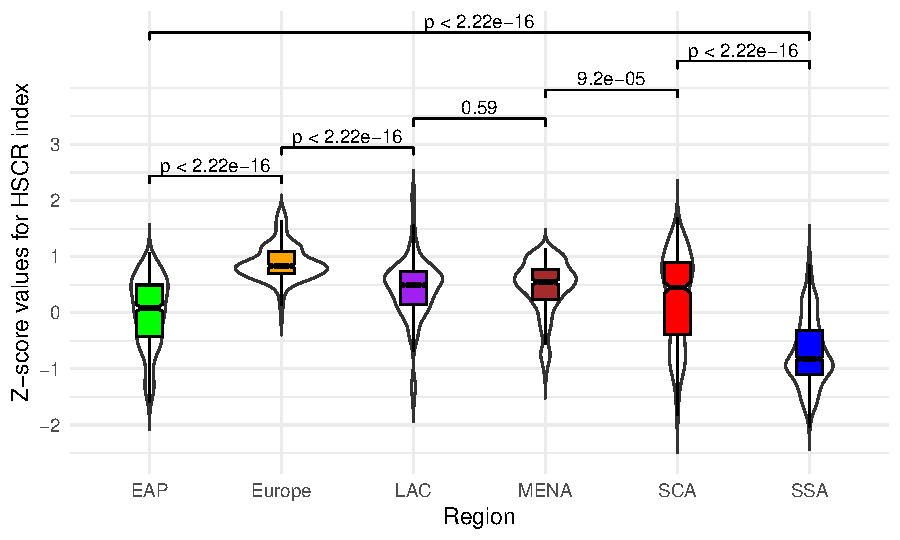
\includegraphics[width = 0.9\textwidth]{Figures/Health_Outcome_Graph/HSCR_Boxplt.pdf}
  %  \label{fig:Health syst Cap}
   % \caption{\footnotesize{Note. Health System Capacity and Responsiveness (HSCR) dimension is derived from six indicators: ODA devoted to health research and basic health activities, birth attended by skilled health personnel, population with access to measles second dose, health facility with essential medicine, health worker density, and family planning access rate. P-value derived from two-way paired t-test. All regions are significantly different at p-value \textless{} 1\%. Author's computation, data from \textcite{unsdg_sustainable_2023, wdi_world_2023}}}
%\end{figure}





%Figure: Health affordability and access
%As illustrated in Figure \ref{fig:CHS}, all regions exhibit a similar level of exposure, with varying levels of intensity distribution among their respective countries. However, the MENA region stands out with a higher incidence of CHS compared to others. CHS incidence is equally high in South and Central Asia (SCA), Europe, Latin America and the Caribbean (LAC), and East Asia and Pacific (EAP), each with a somewhat related nature of distribution among countries. Despite Sub-Saharan Africa (SSA) having the lowest incidence, with most of its countries clustering around the regional median, there are outliers, such as South Africa and Lesotho, with extreme values, ranking among the highest in the world.

%\begin{figure}[ht]    %\captionsetup{justification=justified,singlelinecheck=false}
 %   \caption{\textit{Affordability of Health Care Dimension}}
  %  \vspace{3pt}
   % \centering 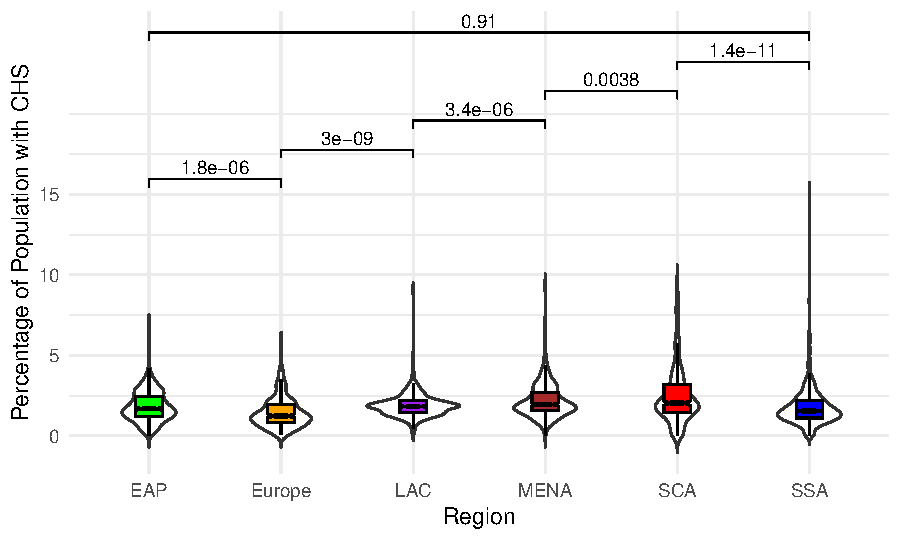
\includegraphics[width=0.8\textwidth, height=7cm]{Figures/Health_Outcome_Graph/CHS_boxplt.pdf}
    %\label{fig:CHS}
    %\caption*{\footnotesize{Note. This dimension is measured solely by the %proportion of the population with Catastrophic Health Spending (CHS) %\footnote{Scholars disagree on what amount of health expenditure %constitutes CHS. OOP \textgreater{} 25\% of household income is used in SDG 3 in line with \textcite{who_world_2010}. And it is adopted in this thesis}. All regions are significantly different at p-value \textless{} 1\%. Author's computation, data from \textcite{unsdg_sustainable_2023, wdi_world_2023}}}
%\end{figure}


Based on the preceding discussion, it is evident that regions exhibit significant differences across various health dimensions, reflecting diverse health situations. Consequently, relying solely on narrow health indicators to assess ODA effectiveness may lead to an underestimation of the intended impact. While the utilization of comprehensive health dimensions does not guarantee disparate results, it remains crucial for ensuring a valid and meaningful inter-region comparison


\subsection*{\quad 2.2.3 Does ODA Flow to Where it is most Needed?}
Previous studies, including \textcite{odokonyero_impact_2018, bavinger_relationship_2017, marty_taking_2017, temple_aid_2010}, have investigated the allocation patterns of foreign aid (ODA) in relation to health situations. In this thesis, a preliminary analysis deems it crucial to further explore the correlation between ODA allocation and various health dimensions. Figures \ref{fig:ODA against Hth dimension} and \ref{fig:Social Infrastructure scatterplt} in the appendix depict the relationship between the Log of ODA per GNI (ODA dependency) and social infrastructure ODA against different health dimensions. The objective is to discern whether countries facing the most significant health challenges receive higher foreign aid, particularly in the form of social infrastructure ODA. The two fitted lines, where the red line represents a linear regression fit and the black line signifies a nonlinear local projection fitted model in each scatterplot, provide insights into the direction and strength of the relationship. Notably, these plots are purely descriptive and are not intended to imply causality.

\begin{figure}[ht]
\captionsetup{justification=justified,singlelinecheck=false}
\caption{\textit{Relationship Between Total Net ODA and Health Dimensions}}
    \centering 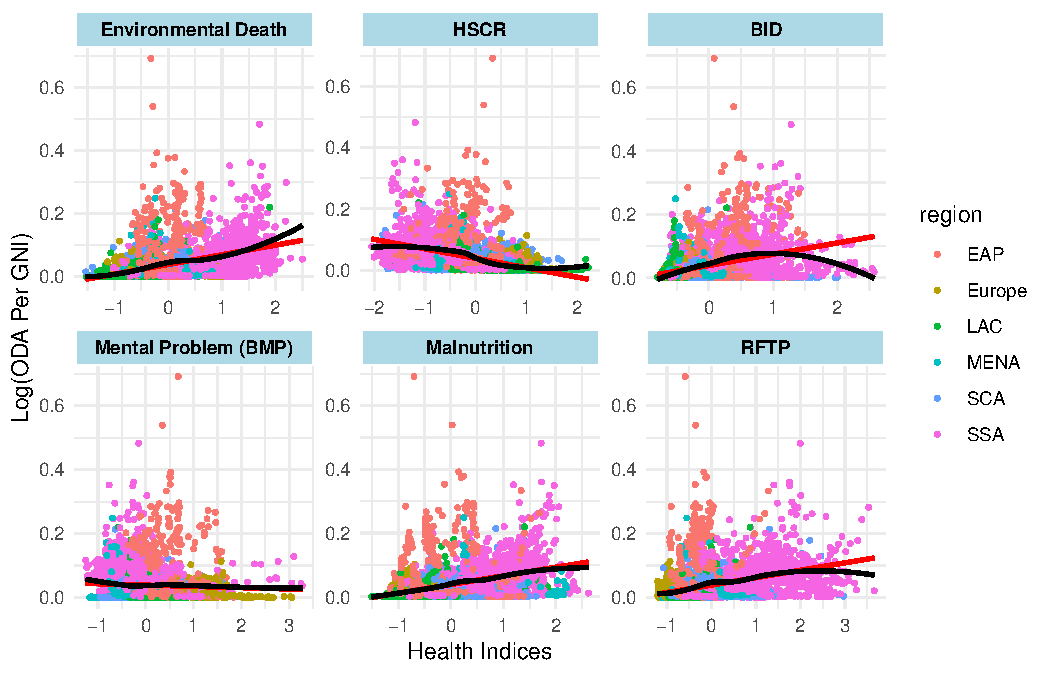
\includegraphics[width =  0.8\textwidth, height = 8cm]{Figures/ODA_against_Hth/ODA_Hth_plt.pdf}
    \label{fig:ODA against Hth dimension}
    \caption*{\footnotesize{Note: Author's computation, data from \textcite{unsdg_sustainable_2023, wdi_world_2023}}}
\end{figure}

From both Figure \ref{fig:ODA against Hth dimension} and Appendix Figure \ref{fig:Social Infrastructure scatterplt}, both total and social infrastructure exhibit a weak correlation and slightly different pattern of relationship across the six health dimensions. Against the position of \textcite{temple_aid_2010}, the finding is supported by a range of others, including \textcite{odokonyero_impact_2018, bavinger_relationship_2017, marty_taking_2017}, who have all argued that ODA flows to where it is less needed. Furthermore, the divergence between the two fitted lines indicates that the relationship between ODA and health problems is not linear. In other words, the flow of ODA does not consistently depend on the burden of health problems. While this suggests a weak statistical association, it does not imply causation.  


%The results revealed a weak negative correlation between ODA across all health dimensions, with correlation coefficients from -0.6 on mental health to 0.30 on under-nutrition (p \textless{} 0.05). 




\subsection*{2.3 Social protection} 
\addcontentsline{toc}{subsection}{2.3 Social protection}
\subsubsection*{\quad 2.3.1 Conceptualizing Social protection}
\addcontentsline{toc}{subsubsection}{2.3.1 Conceptualizing Social protection}
Social protection is a multifaceted concept, shaped by diverse socio-cultural contexts and evolving social risks \parencite{yokobori_roles_2023}. Hence, there is no universally accepted definition and measurement of social protection. The International Labour Organization (ILO), for instance, define social protection as a combination of policies and programs aimed at reducing and preventing poverty and vulnerability throughout the life cycle \parencite[see][]{yokobori_roles_2023, ilo_social_2012}. The ILO Social Protection Floor (SPF), in particular, characterizes social protection as set of minimum social security guarantees, nationally defined to forestall or alleviate poverty, vulnerability, and social exclusion \parencite{ilo_social_2012}. The World Bank, adopting an empowerment approach, defines social protection as a system to help vulnerable individuals cope with life's shocks  and capacity to protect themselves against such shocks \parencite[Discussion in][]{yokobori_roles_2023}. This definition is deeply rooted in Social Risk Management (SRM), viewing social protection as a tool for risk prevention, management, and coping \parencite[]{holzmann_social_2001}.

More succinctly, \textcite{midgley_advanced_2022} defines social protection as resource transfers to individuals or households, ensuring current or future income security. Social protection employs various means, broadly categorized into social assistance, social insurance, and labor market programs, implemented through national policies, international organizations, NGOs, and other authorized state and non-state institutions \parencite{holzmann_social_2001, midgley_advanced_2022, yokobori_roles_2023}. Despite the diverse definitions and functions of social protection, the availability of suitable social protection data for panel analysis poses a challenge \parencite{nino-zarazua_aids_2023}. Given the lack of sufficient panel data for social protection, this thesis utilizes the World Bank ASPIRE data on the total social protection coverage as percentage of population \parencite{wdi_world_2023}, for further analysis.


%social protection development is proxy by the social protection floor, an initiative of the ILO known as Recommendation 202. This framework defines the social protection floor as a set of basic social security guarantees, nationally defined to prevent or alleviate poverty, vulnerability, and social exclusion \parencite{ilo_social_2012}. The framework recommends four minimum levels of social security within national capacities, spanning the lifecycle: access to healthcare, including maternity care; basic child income security; basic active age income security; and basic income security for the older population \parencite{ilo_social_2012}. This framework has been integrated into global development commitments, notably SDG 1.3, leading to the establishment of eight indicators measuring different dimensions of the social protection floor, including the coverage of respective programs outlined in Recommendation 202. The subsequent section provides a descriptive explanation of the distribution of social protection floor indicators.

\subsubsection*{\quad 2.3.2  Social Protection}
\addcontentsline{toc}{subsubsection}{2.3.2 Evolution of Social Protection Development}
\begin{figure}[ht]
\caption{\textit{Relationship Between Social Protection Coverage and Health Dimensions}}
    \centering 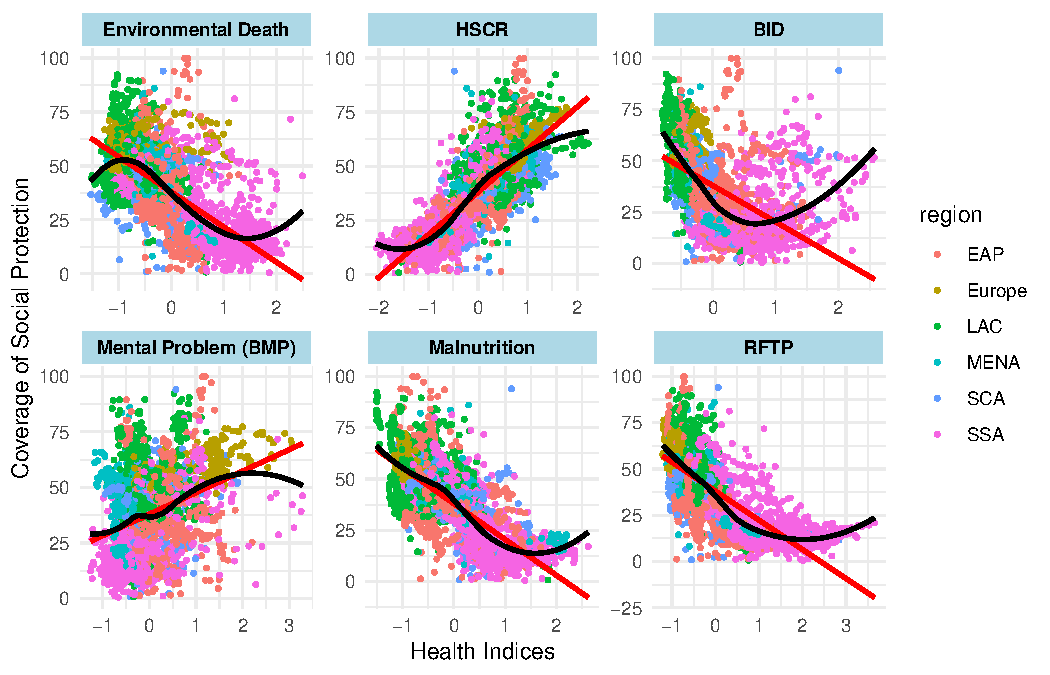
\includegraphics[width = 0.8\textwidth]{Figures/ODA_against_Hth/SocProct_Hlth_plt.pdf}
    \caption*{\footnotesize Note: Social protection coverage is in \% of the total population. Red and black fitted lines are linear and non-linear respectively. Author's computation, data from \textcite{unsdg_sustainable_2023, wdi_world_2023}}
    \label{Fig::SocailProtection and Health}
\end{figure}

The section explains the dynamics of relationship between social protection, health dimensions, and ODA, as shown in Figure \ref{Fig::SocailProtection and Health}, and Appendix Figure \ref{Fig::Social_Prot_Total_ODA} and \ref{Fig::Social_Prot_Social_InfrastructureODA}. Figure \ref{Fig::SocailProtection and Health} shows clear relationship between social protection and various health dimensions. The observed relationship tends to exhibit a non-linear trend, as evidenced by the fitted black lines in Figure \ref{Fig::SocailProtection and Health}. Conversely, in the Appendix Figure \ref{Fig::Social_Prot_Total_ODA} and \ref{Fig::Social_Prot_Social_InfrastructureODA}, neither total net ODA nor social infrastructure ODA  manifests a clear relationship with social protection coverage. It is important to note that this preliminary analysis suggests a potential influence of social protection on health dimensions, with weak evidence on the relationship ODA and social protection. While these graphs are mere descriptive, it does not imply causality. This hypothesis will be further examined and tested  in the subsequent chapters of the thesis.



\subsubsection*{2.4  Conclusion and Summary from Preliminary Analysis}
In essence, the preliminary analysis chapter delves into the complex interplay between the allocation patterns of Official Development Assistance (ODA), health dimensions, and social protection.

\begin{itemize}
    \item The chapter reveal ODA allocation varies with time and reflects global situations. Moreover, Africa and Asia have been the highest recipient of ODA with the United States (US) and Germany being the highest and most predictable donors. Additionally, countries in East Asia and the Pacific (EAP) and Sub-Saharan Africa tend to be more aid-dependent than others. 
    \item By leveraging comprehensive health dimensions, the chapter unveils substantial variations in health situations across regions. Specifically, while reproductive fatality, infection and diseases as well as environmental death are prevalent in SSA, SCA and EAP, mental problem is the major problem in Europe. Moreover, Europe has the best health system capacity, with SSA region being the poorest in this respect. 
    \item The analysis reveals that ODA allocation does not necessarily align with the health needs of recipient countries. 
    \item Finally, While social protection tend to have clear and discernible relationship with all health dimensions, ODA as weak relationship with social protection. While the preliminary offers hint on the pattern of relationship, it does not imply causality. All hypotheses are further tested in the main analysis in Chapter Five. 
\end{itemize}
    
%   The examination of ODA recipients highlights the consistent prominence of Africa, followed closely by Asia, while also emphasizing that the distribution of aid doesn't always align precisely with the regions facing the most pressing health needs.

%Crucially, these findings prompt a reflection on the alignment of international aid with the identified health needs. Our preliminary analysis, as depicted in Figure \ref{fig:ODA against Hth dimension}, \ref{fig:Social Infrastructure scatterplt} and \ref{fig:preliminary stat pair panels}, explores the relationship between ODA allocation and health outcomes. While certain dimensions exhibit a discernible association with ODA, the complex interplay suggests that foreign aid distribution is not solely determined by the magnitude of health challenges in a given region. 

%This insight contributes to the broader investigation into whether foreign aid effectively targets regions with the greatest health needs, as posed in the central research question of the thesis. The nuanced nature of the relationships underscores the multifaceted considerations involved in international aid allocation and sets the stage for a more in-depth exploration in subsequent sections.

\section*{\centering Chapter Three}
\section*{\centering Literature Review}
%\addcontentsline{toc}{section}{Chapter Three}
\addcontentsline{toc}{section}{Chapter Three: Literature Review}
The chapter begins with the conceptual framework, showing the causal logic behind the impact of ODA on health outcomes. The causal chain is further contextualised within the existing body of knowledge, , particularly the relations between the variables of interest and this is organized in line with the research questions. The chapter ends with a summary and conclusion of the literature review. 

\subsection*{3.1 Conceptual/Theoretical Framework}
\addcontentsline{toc}{subsection}{3.1 Conceptual/Theoretical Framework}
The major study variables are the ODA (particularly total and social infrastructure ODA), health outcome \footnote{which is proxy by a composite index with indicators from SDG 3 and SDG 2.1 focusing on health and nutrition respectively}, and social protection \footnote{which is proxy by a composite index created from the social protection floor indicators SDG 1.3.1}, as well as a host of other variables perceived to influence the ODA effect on health outcome (see Chapter Four: Methodology, for more details). ODA is the main predictor variable while health outcome is the main dependent variable and social protection is the mechanism through which the effect of ODA partially or completely improves health outcomes. 
The underlying assumption is that a lack of investment, particularly due to insufficient savings in developing countries, hampers their capacity to provide adequate health and social infrastructures for their populations. Consequently, this results in poor health outcomes and a burden of disease \parencite[]{gama_health_2015}, such as a high level of child and maternal mortality, HIV and tuberculosis. Therefore, ODA presents an alternative investment capital to domestic savings and is expected to enhance health capital and overall health outcome in developing countries \parencite{sachs_case_2014, temple_aid_2010}. This assumption is expressed in the causal chain shown in Figure \ref{fig:Causal graph} below:

\begin{figure}[ht]
\captionsetup{justification=justified,singlelinecheck=false}
\caption{\textit{Causal Chain of ODA Impact on Health Outcome}}
    \centering 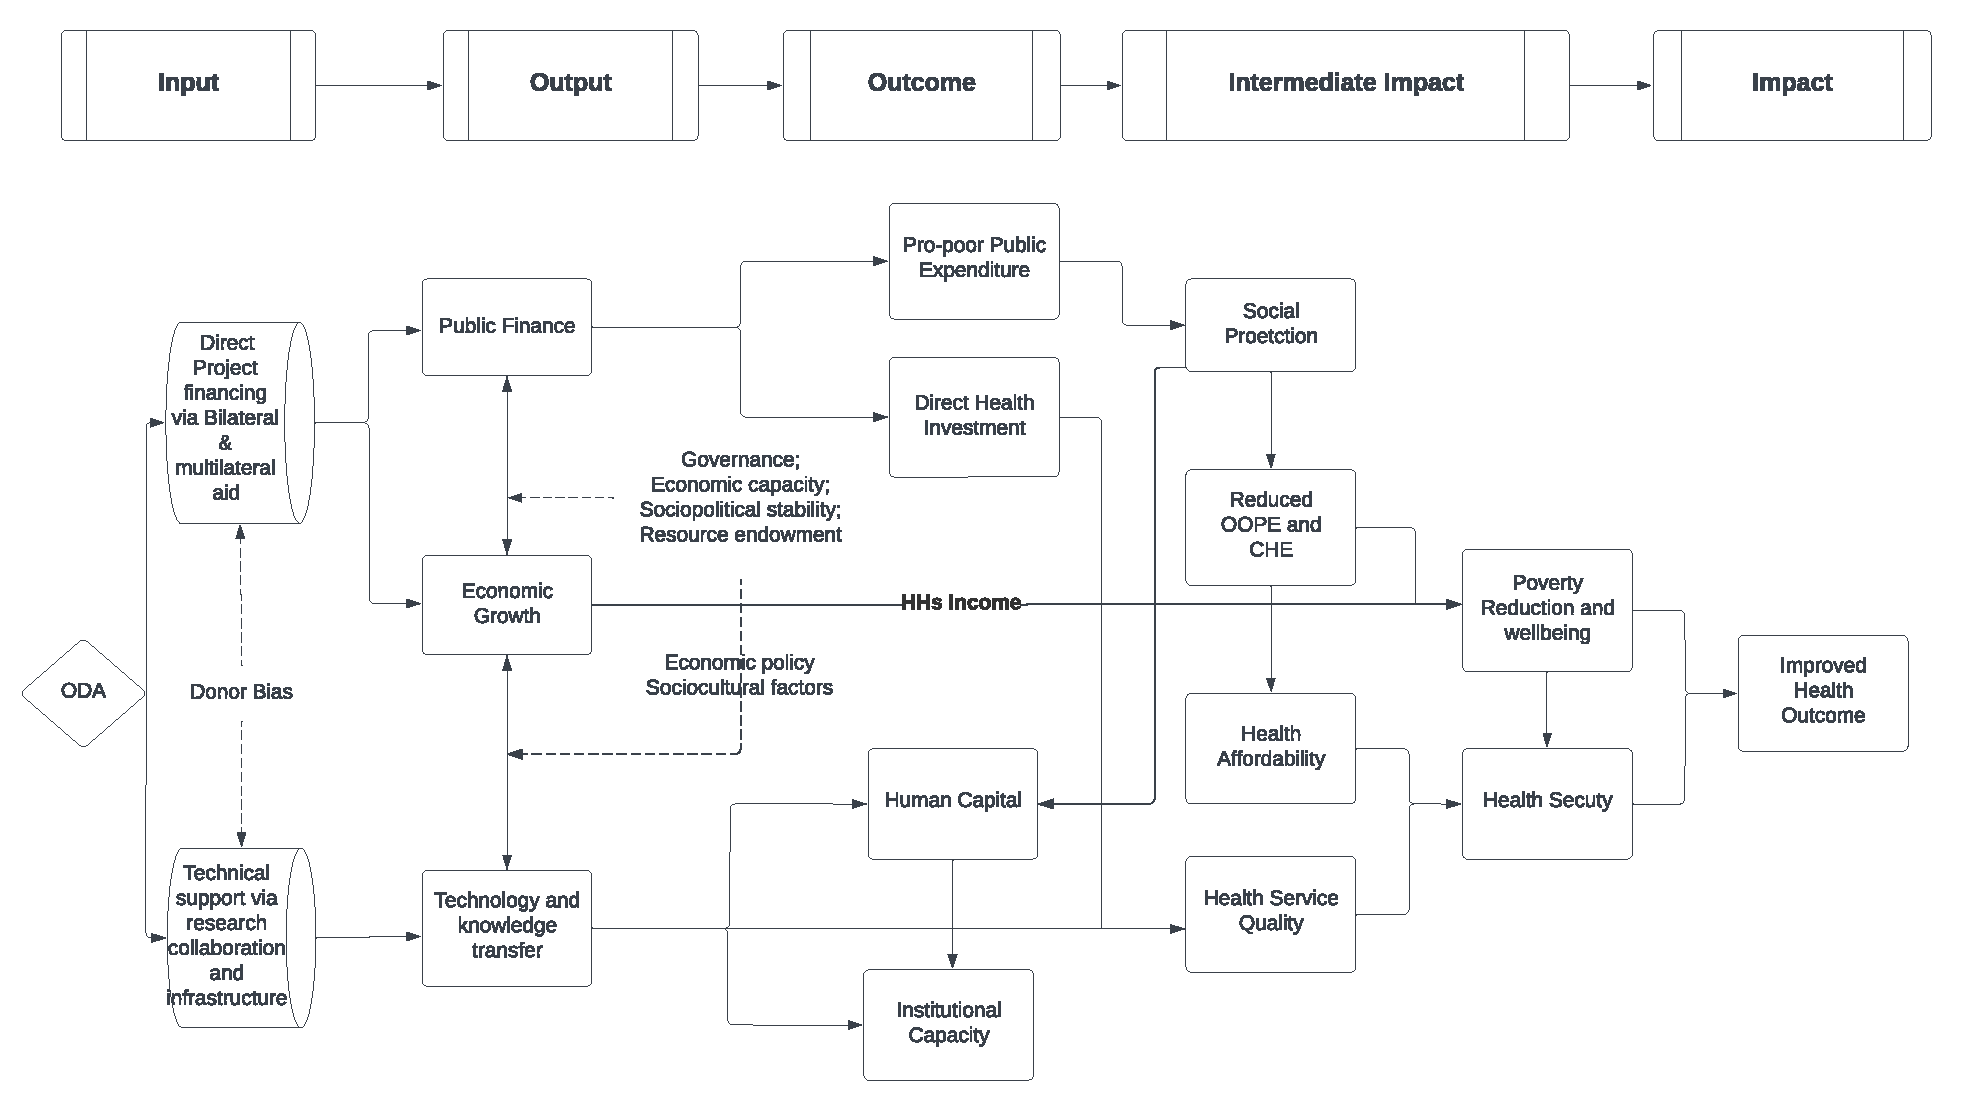
\includegraphics[width = \textwidth]{Figures/Frameworks/Causal Chain Graph for Thesis.pdf}
    \label{fig:Causal graph}
    \caption*{\footnotesize{Note. All variables with dotted lines are assumed to be endogenous factors, capable of moderating the ODA effectiveness on health outcome.\\ Author's illustration.}}
\end{figure}

The conceptual framework draws insights from two economic theories: the Grossman Health Production Theory \parencite{grossman_concept_1972} and the Harrod-Domar Economic Growth Model \parencite{asimakopulos1986harrod}. These theories are synthesized for a comprehensive analysis of the dynamics surrounding health outcomes and ODA.

The Health Demand Theory is a prominent endogenous growth perspective, elucidating the intricate relationship between health outcomes and economic well-being. At its core, the theory posits health as a commodity, produced and consumed by an economic agent \parencite{grossman_concept_1972}. Economic agents produce and consume health, in return for two utilities: (1) freedom from illness and (2) more capacity to work, thus enhancing productivity. Therefore, to maximize optimal health outcomes, economic agents engage in health investments, through various health inputs \parencite{grossman_concept_1972}. While utility from good health remains an agents' motivation for health investment, the capacity for health investment is constrained by the resources available to the agents.

Despite the theory focusing more on micro-level dynamics, it explains the significance of capacity constraints in shaping health outcomes, particularly in developing countries where limited investment capacity in crucial healthcare and social infrastructures contribute to poor health outcomes. Given that health outcomes are intrinsically linked to capability, as equally emphasized by \textcite{sen_health_1998}, pervasive poor health problems in developing countries impede productivity, perpetuating a cycle of poverty \parencite{staicu2017study}.

At a macro level, the Harrod-Domar Growth Model has been influential in understanding the role of investment in economic growth \parencite{asimakopulos1986harrod}. According to the model and its subsequent extension in the two-gap model, insufficient capital accumulation constrains economic growth in developing countries, constituting a development trap  \parencite[see][]{temple_aid_2010}. Therefore, foreign aid is perceived as alternative investment capital to break the countries free from development mysteries \parencite{sachs_case_2014, staicu2017study, temple_aid_2010}.

\subsection*{3.2 Aid Effectiveness Debate: From Economic Growth to Human Development}
\addcontentsline{toc}{subsection}{3.2 Aid Effectiveness Debate: From Economic Growth to Human Development}

The discourse on aid effectiveness in fostering growth and development in developing countries has been a longstanding and debated topic within academia and international development. Originating from an economic perspective in which development deficit in developing countries is attributed to investment gaps, this viewpoint has become the predominant framework for understanding international development for decades \parencite{thuong_impact_2020}. Since then, the debate has continued, leading to a proliferation of perspectives on aid effectiveness. Early scholars assessing aid effectiveness predominantly concentrated on economic growth, viewing it as a tool for poverty reduction \parencite[see][]{yontcheva_macroeconomic_2006}. \textcite{nwude_official_2020} simplifies the divergent views on aid effectiveness into two categories: aid optimists and aid pessimists. 

Aid optimists, grounded in early economic theories, believed that foreign aid could act as an alternative capital to stimulate economic growth and, consequently, eliminate poverty in poor countries \parencite{temple_aid_2010}. In the 2000s, scholars like \textcite{sachs_case_2014, sachs_geography_2001} were vocal advocates of this perspective. Conversely, aid pessimists, citing the widespread poverty in Africa and South Asia despite decades of aid, contend that aid has been ineffective or has even damaged economic growth in the recipient countries \parencite{easterly_aid_2004, easterly_are_2007, easterly_can_2009}.

Beyond these prevailing viewpoints, \textcite{yontcheva_macroeconomic_2006} classified emerging findings into new group defined as aid conditionality and nonlinearity academia. According to these studies, aid effectiveness is contingent on contextual factors in both the receiving and donor countries. Among the relevant factors observed are recipients' governance, initial economic growth, socio-cultural dynamics, and donor conditionality \parencite{yontcheva_macroeconomic_2006, abate_relationship_2022, nwude_impact_2023, temple_aid_2010}. Today, the terrain of academic argument has been replicated beyond aid effectiveness on economic growth \parencite[see][]{yontcheva_macroeconomic_2006, temple_aid_2010}, to other development indicators, including the Human Development Index (HDI), health, inequality and social development \parencite[i.e.][]{aluko_analysis_2021, habtetsion_impact_2017, shafiullah_foreign_2011}. Since the focus of this thesis is on health outcome, the following section discusses the dynamics of aid effectiveness on health outcome in more detail.


\subsection*{3.3 Effectiveness of ODA on Health Outcome}
\addcontentsline{toc}{subsection}{3.3 Health Outcomes as a Focus of Aid Effectiveness}
In the era of Sustainable Development Goals (SDGs), the global focus on addressing public health issues and inequality has increased ODA to social development sectors, particularly the health sector, as depicted in Figure \ref{fig:ODA sectors commitment} (see discussion in Chapter Two). This shift necessitates investigating whether the renewed development interest has indeed realized the intended benefits on health outcomes in recipient countries. Numerous studies have examined the impact of aid on health outcomes using various health indicators, including traditional indicators like incidence of maternal and child mortality, HIV and Tuberculosis, life expectancy, and immunisation coverage \parencite{nwude_official_2020, yan_mortality_2015, doucouliagos_health_2021, kavakli_us_2022, williamson_foreign_2008}. Other general social development indicators from the HDI \footnote{HDI, as a development index, comprises three dimensions, each measured by distinct indicators: Knowledge measured by education, health measured by life expectancy and wellbeing measured by per capita income. Data is computed by UNDP} \parencite{kavanagh_governance_2019, chung_economic_2022, mohamed_foreign_2017} to health promotion research \parencite{cassola_evaluating_2022} have equally been used as measures of health outcome, with inconclusive results. However, it is essential to understand the context of these diverse findings.


\textcite{yan_mortality_2015} assessed the impact of the Global Health Fund, one of the largest multilateral donors in global health, on the rate of change in mortality. The study used all causes of death among adults, under-5 child mortality, and malaria-specific under-five mortality as proxies for mortality. Analyzing data from 1995 to 2010 for all eligible aid countries with fixed effects, the study found a significant positive effect of the Global Health Fund on adult mortality and malaria-specific child mortality. Specifically, an increase of 10 USD in global fund allocation reduced adult mortality and malaria-specific child mortality by 1.4 and 6.9 percent points (p.p) annually \parencite{yan_mortality_2015}. In a similar finding, \textcite{kavanagh_governance_2019} revealed that the global health funding significantly reduces adult mortality, together with the overall HDI, part of which is health. In further macro analysis examining the effect of health aid on infant mortality using fixed effects and two-stage least square with data from 2002 to 2015 for 95 countries, \textcite{doucouliagos_health_2021} revealed that ODA is effective in reducing child mortality.

%%%%%%%%%%% We stopped here with Prof %%%%%%%%%%%%%
In a different study, \textcite{kavakli_us_2022} investigated the impact of the Mexico City Policy (MCP) \footnote{Mexico City Policy (MCP) is a policy in the US, which reduces or removes its ODA for reproductive health promotion, such as access to family planning and abortion \parencite{kavakli_us_2022}}, with data from 1990 to 2015 for 134 countries. Using fixed effects, the authors found that MCP had a significant positive effect on maternal and child mortality as well as HIV incidence, with the impact being more pronounced in countries highly dependent on US aid \parencite{kavakli_us_2022}. These findings are supported by several other studies \parencite{akinola_foreign_2022, mohamed_foreign_2017, muhammad_health_2021, yogo_health_2015}, who have all found the positive impact of ODA on their respective health indicators.

In contrast to the optimistic studies, numerous other investigations have reported the ineffectiveness of aid across various health outcome indicators. One of the earliest pessimistic findings was presented by \textcite{williamson_foreign_2008}. The author assessed the impact of both health and total ODA on health outcomes, utilizing five health indicators: life expectancy, infant mortality, death rate, immunization of measles, and immunization of DPT. The data spanned from 1973 to 2004 and was analyzed using fixed effects. The study concluded that neither total nor health-related ODA significantly influenced health outcomes in developing countries. Instead, only Gross Domestic Product (GDP) was found to significantly reduce infant mortality, with a 1\% increase in GDP leading to a 0.337\% reduction in infant mortality \parencite{williamson_foreign_2008}. More than a decade later, Nwude et al. (2020) supported these findings. Utilizing the Generalized Method of Moments (GMM) to assess the impact of ODA on child mortality and life expectancy, the authors revealed that ODA does not enhance health outcomes. However, control variables such as immunization and the prevalence of HIV were found to influence health outcomes \parencite{nwude_official_2020}. Concentrating on the effect of ODA on Out-of-Pocket Health Expenditure (OOPHE) with data from 1995 to 2015, analyzed with fixed effects and instrumental variables (IV), \textcite{ali_foreign_2020} found no robust effect of ODA on OOPHE. These conclusions are corroborated by various other studies, collectively discrediting the notion of ODA significantly impacting health outcomes \parencite{bavinger_relationship_2017, chung_economic_2022, rosala-hallas_global_2018, toseef_how_2019}.

In the pursuit of understanding aid effectiveness on health outcomes, several studies have ventured into exploring various health-related indicators. In a qualitative study focused on assessing the ODA research grant mechanisms on global health, \textcite{cassola_evaluating_2022} revealed that ODA research grants positively influence the research landscape by elevating research institutions, promoting interdisciplinarity, and increasing the volume of research. However, this effectiveness was observed primarily for donor countries, with no significant evidence of direct welfare development in recipient countries \parencite{cassola_evaluating_2022}. In a different study, \textcite{bavinger_relationship_2017} examined the relationship between child health ODA allocation and the global burden of disease \footnote{The global burden of disease was proxied by vaccine-preventable diseases such as newborn diseases \parencite{bavinger_relationship_2017}}. The authors concluded that there is no significant relationship between child health ODA allocation and the global burden of disease \parencite{bavinger_relationship_2017}.

Amidst the ongoing macro-analysis debate, a parallel exploration of the micro-level impact of ODA has yielded a mix of findings. \textcite{akinola_foreign_2022} directed their analysis towards evaluating the effect of ODA on health outcomes, proxied by life expectancy, in Nigeria, using Auto Regressive Distributive Lag (ARDL). The authors concluded that ODA had no significant effect on life expectancy in Nigeria, with government expenditure emerging as the influential factor. In Uganda, \textcite{odokonyero_impact_2018} investigated how health ODA impacted the prevalence and burden of diseases, utilizing household survey data spanning from 2005 to 2014 through the Difference-in-Difference (DID) approach. Despite the observation that health ODA may not always be allocated to where it is needed the most, the author found that health ODA not only significantly affected the productivity burden of disease but also hastened recovery times rather than preventing diseases. Moreover, aid was found to be more effective for those living close to the project areas \parencite{odokonyero_impact_2018}. 

Conversely, despite using a similar DID method, \textcite{marty_taking_2017} reported 
different findings in Malawi, focusing on the effect of infrastructure and parasitic ODA on the incidence of malaria and perceived adequacy of healthcare with a two-wave household survey in 2010/2011 and 2004/2005. Regardless of foreign aid being less allocated to the least developed areas, infrastructure and parasitic aid were associated with a reduction in malaria prevalence by 1.20 to 12.1 percentage points (Marty et al., 2017). This finding gains additional support from the work of \textcite{muhammad_health_2021}, who, in a study conducted in Nigeria, observed a significant influence of health-related ODA on health outcomes in both the short and long term.

%%%%%%%%%%%%%%%%%%%%%% Conditions moderating ODA %%%%
\subsubsection*{- Conditionality and Nonlinearity of ODA Effectiveness}
\addcontentsline{toc}{subsubsection}{Conditionality and Nonlinearity of ODA Effectiveness}

To address the controversies surrounding the ODA's effectiveness on health outcomes, several studies have delved into explaining the conditions that moderate this impact. \textcite{doucouliagos_health_2021} attributed the mixed or ineffective findings in previous studies to the absence of governance in their models, making governance a crucial moderating variable in the effect of ODA on health. Utilizing fixed effects and two-stage least squares (2SLS) with data spanning from 2002 to 2015 for 95 countries, the authors revealed that the impact of health ODA on infant mortality is contingent on governance, particularly government effectiveness and corruption levels \parencite{doucouliagos_health_2021}.

In a dynamic panel model, \textcite{abate_relationship_2022} demonstrated that the effect of ODA on enhancing economic growth becomes negative only when governance and economic freedom indicators fall below a certain threshold. The author concluded that government effectiveness is essential to observe aid effectiveness. Similarly, to consider the role of government effectiveness and capacity in the effect of ODA on the Human Development Index (HDI), \textcite{chung_economic_2022} interacted their main predictors, ODA and Gross Domestic Product (GDP) per capita. In both models, the study revealed that government effectiveness and capacity magnified the effect of ODA on HDI \parencite{chung_economic_2022}. This finding is supported by \textcite{muhammad_health_2021}, where governance indicators such as government effectiveness, corruption, accountability and voice, rule of law, and regulation quality competitively reduced under-5 child mortality. In their study, \textcite{kavanagh_governance_2019} even asserted that the global health fund reduced child mortality while simultaneously improving government effectiveness, corruption control, and the rule of law. Furthermore, in a systematic study on ODA effectiveness in poverty reduction, \textcite{mahembe_foreign_2019} emphasized the role of democracy in enhancing aid effectiveness.

In contrast, this perspective was debunked over a decade ago by \textcite{williamson_foreign_2008}, who combined five health indicators as outcomes and found that governance indicators, such as the Fraser freedom index and political freedom, did not influence health outcomes \parencite{williamson_foreign_2008}, subsequent studies have reiterated this finding. For instance, in a similar study, \textcite{david_contribution_2017} found governance to be insignificant in moderating ODA effectiveness. This observation was also supported by \textcite{ali_foreign_2020}, where institutional quality was deemed insignificant in influencing health outcomes or the effectiveness of foreign aid on health.

Another dimension to consider is highlighted by \textcite{yogo_health_2015}, who compared the effects of ODA on health outcomes, using HIV incidence, child mortality, and life expectancy as proxies, between post-conflict and stable states. Using a Generalized Method of Moments (GMM) combining both system and first differencing methods, the authors found that ODA significantly improved health indicators in post-conflict states. Similarly, \textcite{bavinger_relationship_2017} suggested that Child Health ODA could have the intended effect if allocated to the burden of diseases. Using quartile regression, \textcite{mohamed_foreign_2017} revealed that the effectiveness of foreign aid was observable in the 25th, 50th, and 75th quantiles, while the effect declined along the ranking, confirming the nonlinearity of aid effectiveness.



\subsection*{3.4 Social Protection's Mediating Role in ODA's Impact on Health Outcomes}
\addcontentsline{toc}{subsection}{3.4 Social Protection's Mediating Role in ODA's Impact on Health Outcomes}
In recent times, the convergence of health economics/public health and social protection has become increasingly prominent, breaking down the silos that traditionally separated these fields. This integration is partly championed by endogenous growth economists such as Grossman (1972), Östlin et al. (2004), A. Sen (1996), K. Sen, and Koivusalo (1998), and Wagstaff (2002), through contributions on poverty, economic conditions and health outcome. Development organizations and scholars have advocated for social protection as a crucial instrument, particularly in advancing Universal Health Coverage (UHC). The rationale is that social protection plays a pivotal role in poverty eradication and reduction, thereby promoting UHC by eliminating financial barriers to healthcare services, ensuring access, affordability, and health equity \parencite{fox_clinical_2015, ilo_towards_2020, lonnroth_beyond_2014, siroka_association_2016, world_bank_high-performance_2019, who_world_2010}.

\subsubsection*{\quad 3.4.1 Social Protection and Health Outcome}
\addcontentsline{toc}{subsubsection}{3.4.1 Social Protection and Health Outcome}

The interconnection between social protection and health has gained momentum, especially in the aftermath of the Covid-19 pandemic \parencite[see][]{mccord_official_2021, yokobori_roles_2023}. One significant consensus from the literature is that social protection contributes to the discourse on public health in two main ways. Firstly, the evolution of social protection has reinforced the realization of a rights-based approach to health, particularly with the integration of health into various social protection frameworks \footnote{A significant example is the ILO Social Protection Floor (SPF recommendation 202), which is now integrated in SDG 1.3} \parencite[discussion in][]{hagemejer_role_2013, ilo_social_2012, macnaughton_decent_2010, ilo_towards_2020, yokobori_roles_2023}. Secondly, and particularly relevant to this thesis, social protection contributes to the development of health financing models, notably social security and social assistance—both integral components of Social Protection \parencite{scheil-adlung_focusing_2020, scheil-adlung_response_2014, world_bank_high-performance_2019, who_world_2010}. Consequently, studies examining the impact of social protection on healthcare outcomes can be categorized into two main groups: those focusing on social insurance and those examining social assistance. While each stream of research offers valuable insights, the evidence remains inconclusive.

\paragraph{\quad \quad \textit{3.4.1.1	Social Insurance and health outcome}} 
\subparagraph{}
Although the impact of social insurance on health outcomes is mixed, with significant controversy around its efficacy in safeguarding vulnerable and impoverished populations from Catastrophic Health Spending (CHS) \parencite{korachais_impact_2019, sarkodie_effect_2021}. The controversy is not surprising, given that the subsidization or elimination of medical user fees might be perceived as a windfall gain, leading to increased utilization of healthcare services in terms of both quantity and quality by households. A systematic review by Azzani and colleagues identified health shocks as a major cause of high health consumption among poor households, thereby inducing CHS \parencite{azzani_determinants_2019}. In a similar study conducted in China, \textcite{xu_equity_2021} reported that poor households disproportionately consumed health services compared to other income groups. This observation may explain the findings of \textcite{helmsmuller_does_2022} in the evaluation of the Social Protection Health Initiative (SPHI) in Pakistan, where despite the provision of free inpatient insurance, the quantity of care remained relatively constant, with most households shifting from public to private healthcare. If social insurance indeed protects freedom of choice and enhances care quality, as reported by \textcite{helmsmuller_does_2022} and others \parencite{gajate2015effect, korachais_impact_2019}, then its impact is noteworthy.

Conversely, other studies have reported the positive impact of social insurance on health outcomes extending beyond freedom of choice. In a study conducted in Vietnam, analyzing survey data from 46,000 households with multivariate regression, \textcite{sepehri_how_2014} concluded that the use of social insurance cards reduced Out-of-Pocket (OOP) health expenditure by 50 to 56\% compared to a counterfactual group. Similarly, in the seventh round assessment of the National Health Insurance Scheme (NHIS) in Ghana, \textcite{sarkodie_effect_2021} reported that NHIS increased health demand by 26\% while reducing OOP spending by 4\%. These findings are complemented by many others \parencite{dror_impact_2016, frolich_effects_2018, habib_role_2016, levine_insuring_2016}, indicating that the provision of health insurance offers financial protection from CHS, improves service access, and leads to various positive social outcomes. In fact, \textcite{dror_impact_2016} conclude that health insurance has the potential to generate welfare gains that could elevate poor households up the income ladder.

 
\paragraph{\quad \quad \textit{3.4.1.2	Social Assistance and Health outcome}}
\subparagraph{}
Social assistance is widely recognized as a set of programs or policies that offer non-contributory transfers, in the form of either or both in-kind and cash assistance, to improve the livelihoods of individuals considered vulnerable or living in chronic poverty \parencite{heggebo_disentangling_2020, shahidi_impact_2019, world_bank_state_2015} \footnote{Social assistance provision serves as protective measure, thus, it means-targetted and could be short term}. Health shocks affect poor individuals in two ways: first, through the financial burden of direct healthcare service costs, and second, through indirect costs resulting from the loss of income due to low productivity or an inability to work \parencite{helmsmuller_does_2022}. Therefore, social assistance provides a safety net, as described by the \textcite{world_bank_state_2015}, protecting the poor and vulnerable during challenging times. Assessing the impact of social assistance on health outcomes is particularly novel.

\textcite{adato_social_2009} summarized the health impact of cash transfers as protecting against the direct costs associated with accessing health services and enhancing self-health management behaviours among the poor through health education and conditional assistance. Similarly, in the review of \textcite{shahidi_impact_2019}, four experimental and quasi-experimental studies found that a reduction in the adequacy of social assistance benefits had adverse health effects, emphasizing the importance of ensuring adequate benefits for optimal outcomes. In Sub-Saharan Africa (SSA), \textcite{owusu-addo_impact_2018} revealed that the provision of cash transfers improved healthcare consumption and financial protection. 
Therefore, social protection, through the combination of different instruments, offers a comprehensive approach to enhancing health outcomes and addressing inequities in health systems \parencite{hagemejer_role_2013, world_bank_high-performance_2019, yokobori_roles_2023, ilo_towards_2020, who_world_2010}. 

\subsubsection*{\quad 3.4.2 ODA Effectiveness on Social Protection:}
\addcontentsline{toc}{subsubsection}{3.4.2 ODA Effectiveness on Social Protection}
Despite its crucial role, establishing a sustainable and stable social protection system requires substantial capital investment, a resource often lacking in developing countries (McCord et al., 2021). As of 2020, the International Labour Organization (ILO) estimated a financing gap of USD 1,191.6 billion or 3.8\% of GDP in low and middle-income countries for social protection floors, including Universal Health Coverage \parencite{duran-valverde_financing_2020}. The demand for ODA is crucial, especially in the COVID-19 pandemic, where an increase in ODA flow has enabled many low-income countries to enhance their social protection systems \parencite{mccord_official_2021}. Despite the growing demand for ODA for social protection, few studies have explored its impact, and existing ones often use general poverty or human development indicators as proxies for social protection \parencite{forte_impact_2023, lonnroth_beyond_2014, mahembe_foreign_2019, shafiullah_foreign_2011}.

Niño-Zarazúa and colleagues conducted a study assessing the effect of ODA on social protection, proxy by coverage of non-contributory programmes, in low and middle-income countries, using an instrumental variable with a Tobit regression model. The findings revealed that ODA has contributed to the expansion of social protection systems in developing countries. Specifically, a 1\% increase in ODA allocated to social protection increased coverage by 0.25\% points, with the highest impact observed in Sub-Saharan Africa (0.26\%) \parencite{nino-zarazua_aids_2023} \footnote{One significant limitation in the study and others aiming to study social protection is the lack of panel data on various social protection performance indicators. Both ILO and World Aspire data are only suitable for cross-sectional analysis \parencite{nino-zarazua_aids_2023}}. A systematic literature review on aid effectiveness in poverty reduction by \textcite{mahembe_foreign_2019} classified studies based on monetary and non-monetary poverty indicators, showing that ODA has contributed to poverty reduction in most studies, regardless of the poverty indicator used. 

\textcite{david_contribution_2017} investigated the effect of ODA on poverty reduction in ECOWAS countries in SSA region, covering data from 1980 to 2014. The study revealed that ODA reduced poverty through the channel of infant mortality. Additionally, both ODA and Foreign Direct Investment (FDI) increased domestic investment in the studied region \parencite{david_contribution_2017}. In a similar study, \textcite{mohamed_foreign_2017} explored the impact of ODA per capita on human welfare, particularly in poverty reduction, using quartile regression. The study found that ODA has a significant impact on human welfare across all quartiles, although the impact is nonlinear. Focusing on the role of ODA in reducing GINI inequality, \textcite{shafiullah_foreign_2011} employed a combination of fixed and random effects. The study found a negative relationship between ODA and inequality, with the conclusion that inequality is inevitable at the initial stages of a country's growth, aligning with the Environmental Kuznets Curve (EKC) hypothesis.

In contrast to the findings above, \textcite{forte_impact_2023} examining the impact of Foreign Direct Investment (FDI) on social welfare, proxied by HDI \footnote{Virtually all studies on Social welfare used HDI, encompassing income, health, and education} data from 2002 to 2019 for 146 countries, found that FDI harmed social welfare and human development. This negative impact was only reversed in countries with already high human capital. The authors concluded that as FDI increases wage inequality, it fails to improve the situation of poor people due to their lack of the required absorptive human capital \parencite{forte_impact_2023}. Similarly, in the work of \textcite{alves_impact_2023}, focusing on the impact of foreign aid on aggregate welfare, proxy by HDI, the authors found no evidence that ODA enhances human development. This finding is consistent with \textcite{gama_health_2015}, who did not identify any significant effect of ODA on African household income, measured by Gross National Income (GNI), or education.

In a quest to assess the competing effect of both FDI and ODA on poverty reduction with data spanning 1990 to 2017 for 29 countries in SSA, \textcite{anetor_impact_2020} found no significant effect of either ODA or FDI on poverty reduction in Africa. The authors concluded that the required amount of FDI for poverty alleviation in Africa has not been reached, and the flow of ODA has not been channelled effectively. Taking a more comprehensive approach, \textcite{iwegbu_effectiveness_2022} reported that foreign aid, when combined with effective fiscal policies on education and health, significantly enhanced household income in all African regions. This underscores the necessity of combining policies for optimal social outcomes. This perspective aligns with the findings of the systematic review by \textcite{mahembe_foreign_2019}, where the authors concluded that ODA allocated to pro-poor sectors, such as education, health, and other social services, proves to be more effective for poverty reduction.



\subsection*{3.5 Regional Heterogeneity of ODA Impact}
\addcontentsline{toc}{subsection}{3.5 Regional Heterogeneity of ODA Impact}
\paragraph{} An entrenched belief in academia that aid ineffectiveness may be specific to certain regions, is repeatedly expressed by \textcite{easterly_can_2009, easterly_aid_2004}, who justified aid ineffectiveness by citing perpetual poverty and state development challenges, particularly in Africa, despite foreign aid. This viewpoint has spurred renewed academic interest in studies controlling for regions when assessing aid effectiveness, yet the pattern of findings remains inconclusive.

In a study by \textcite{yan_mortality_2015} on the impact of the Global Health Fund on adult and child mortality as well as HIV incidence, two models were employed—one comprising all countries and the second restricted to the SSA region. The general model revealed a significant effect of the global health fund on the measured indicators. Specifically, a 10 USD per capita increase in the global health fund is attributed to a 6.9 percentage points reduction in malaria-specific child mortality. However, in the SSA-specific model, the effect was reduced to 3.6 percentage points \parencite{yan_mortality_2015}. Analyzing social protection coverage and ODA with an Instrumental Variable (IV)-Tobit model, \textcite{nino-zarazua_aids_2023} found that the effect of ODA on social protection coverage was the highest in SSA compared to the Pacific, Latin America and the Caribbean (LAC). Specifically, a 1\% increase in ODA allocation increased social protection coverage by 0.26\% in SSA, 0.24\% in the Pacific, and 0.12\% in LAC.

More broadly, \textcite{doucouliagos_health_2021} controlled for dummy variables capturing regional variations across SSA, Middle East and North Africa (MENA), LAC, Europe and Central Asia, South Asia, North America, East Asia and Pacific. Their data, covering 2002 to 2015 for 95 countries, revealed that the effectiveness of foreign aid was observable across regions when conditioned on governance and was not significantly different across regions. Similarly, \textcite{mohamed_foreign_2017}, employing a similar procedure, revealed that aid effectively improved people's income and had the potential for poverty reduction across regions.


In a more comprehensive study focusing on SSA, \textcite{nwude_impact_2023} examined the impact of aid channels, specifically bilateral and multilateral while considering regional differences between Francophone and Anglophone SSA. Using a Pooled Mean Group (PMG) approach, the study revealed that bilateral aid had a positive and significant effect in Francophone SSA, whereas it exhibited a weak negative effect in Anglophone SSA. The negative effect of multilateral aid was stronger in Anglophone SSA compared to Francophone SSA \parencite{nwude_impact_2023}. These findings align with \textcite{yogo_health_2015}, where health ODA significantly reduced child mortality, albeit the impact is more visible in post-conflict states than in stable states. In another study, \textcite{chung_economic_2022} investigated the socioeconomic impact of ODA in Africa using a spatial autocorrelation panel model. They found that ODA had a significant and positive effect on the Human Development Index (HDI), although no effect on GDP per capita.

Contrastingly, \textcite{nwude_official_2020} compared SSA and non-SSA regions in the effect of ODA and income per capita on health outcomes. While health ODA did not improve life expectancy, income per capita did, and this finding was consistent across regions. However, the effect of ODA was reported to be higher in SSA than in non-SSA regions \parencite{nwude_official_2020}. This aligns with \textcite{staicu2017study, gama_health_2015}, who posited that foreign aid does not improve education or household income in Africa. More intricately, \textcite{shafiullah_foreign_2011} evaluated the effect of ODA on inequality reduction, considering regional variation in results. The findings indicated that while the first lag of ODA significantly reduced inequality in the general model, the second lag order of ODA increased inequality in South Asia, with similar findings for GDP. 

\subsection*{3.6 Summary and Conclusions from the Literature Review}
\addcontentsline{toc}{subsection}{3.6 Summary and Conclusions from the Literature Review}
\paragraph{} In summary, the literature review extensively explores the intricate relationship between Official Development Assistance (ODA) and health outcomes, highlighting the potential mediating role of social protection. The debate on aid effectiveness is thoroughly examined, encompassing macro and micro-level analyses with divergent perspectives from optimists and pessimists. The review delves into conditions moderating aid effectiveness, emphasizing the nuanced assessments required, especially in the context of regional variations. Amidst these debates, social protection emerges as a crucial mediator, bridging health and economic well-being. The intersection of poverty and health conditions underscores the role of social protection in promoting health equity. Despite the mixed impact of social insurance in protecting the vulnerable against CHS, both social insurance and social assistance provides the opportunity to enhance health outcome and address health inequity.

As the literature remains inconclusive, the thesis adopts a unique perspective by navigating the complexity of health outcome definitions, considering regional dynamics of health problems, and recognizing the mediating role of social protection. This approach is crucial for understanding aid effectiveness and informing policymaking in the realm of international development. The synthesis of evidence provides a foundation for the empirical investigation within the thesis, aiming to contribute meaningfully to the ongoing discourse on aid impact and health outcomes.
\section*{\centering Chapter Four}
\section*{\centering Research Methodology}
%\addcontentsline{toc}{section}{Chapter Four}
\addcontentsline{toc}{section}{Chapter Four: Research Methodology}

%The primary causal objective is to estimate the Average Causal Response to Treatment (ACRT), where ODA allocation serves as the treatment variable. ACRT, in contrast to Average Treatment Effect (ATE) causal inference, is an extension of Average Treatment on the Treated (ATT). It specifically aims to capture the average marginal effect on the outcome variable (health) for the treated group, representing the actual recipients of ODA, over a specified time period \parencite[see][]{imbens2015causal, morgan2015counterfactuals}.

\subsection*{4.1 Empirical Strategy}
\addcontentsline{toc}{subsection}{4.1 Empirical Strategy}
The study is, by nature, a quantitative macro-econometric analysis, focusing on the trajectory of the impact of ODA on health outcomes in developing countries over time. To achieve this objective, a panel model approach is employed, leveraging observational panel data, also known as longitudinal or time series cross-sectional data. This approach is chosen for its ability to model the dynamic behaviors of study units denoted as $i$ for the cross-sectional dimension, at different time points denoted as $t$, representing the time series dimension \parencite{hsiao2007panel, cameron2005microeconometrics, blackwell2018make, allison2017maximum}. According to \textcite{gujarati2004econometrie}, panel (or two-dimensions) data enhances both the quantity and quality of inference in the following ways:

\begin{enumerate}[i]
    \item The pooling of various entities across different times increases the number of observations, which in turn, provides higher statistical power and inference precision \parencite{gujarati2004econometrie, hsiao2007panel, cameron2005microeconometrics}.
    
    \item Additionally, by studying specific behaviors of interest across entities at different times, panel data mitigates potential unobserved variable bias, by controlling for differences among units (heterogeneity) that are time persistent \parencite{hsiao2007panel, allison2017maximum}.
    \item Panel data is effective in addressing reverse causality, a situation where the causal order between two variables $X$ and $Y$ is bidirectional, other than unidirectional \parencite{berrington2006overview, allison2017maximum}. Furthermore, the sequence of the causal order or predominance could also be modeled \parencite{berrington2006overview, seddig2020maximum}.  
\end{enumerate}

Despite the merit of panel data, the traditional endogeneity problem does not entirely disappear \parencite{berrington2006overview}. Panel models can be broadly categorized into two: static and dynamic panel model \parencite{seddig2020maximum}. Before delving into specific panel models for each research question, it is imperative to discuss the underlying assumptions of each panel approach. In a simple static panel model, the standard assumption is that $f(y_{it}|x_{it}, \epsilon_{it})$ with $E[\epsilon | x_{it}]  = 0$:
\begin{equation}
    y_{it} = \alpha + \beta^T x_{it} + \epsilon_{it},
    \begin{cases}
        i & = 1, 2, 3, \ldots, N \\
        t & = 1, 2, 3, \ldots, T \\
    \end{cases}
    \label{eq1}
\end{equation}

Here, $\beta^T$ represents the average effect for all units (countries) $i$ at all time (year) $t$. In our context, $x$ denotes ODA allocation, while $y_{it}$ is the health outcome (HO), $\alpha$ is constant across time and units and accounts for baseline health outcome in the absence of ODA (when $x=0$).
  
\subsection*{4.2 Model Assumptions}
\addcontentsline{toc}{subsection}{4.2 Model Assumptions}
\subsubsection*{\quad 4.2.1  Unit Homogeneity vs Heterogeneity}
\addcontentsline{toc}{subsubsection}{4.2.1 Unit Homogeneity vs Heterogeneity}
The simple static panel model in Equation \ref{eq1} assumes unit homogeneity, implying a consistent parameter across units. However, this assumption is practically unrealistic \parencite{hsiao2007panel}. Health is a complex reality, influenced by multiple factors, and varies, to some degree, across countries and regions, as discussed in Chapter Two. 
Moreover, given that ODA allocation is based on country eligibility, including country income level \parencite{oecd_ODA_Report_2023} and other countries' specific factors (both observable and unobservable), the probability density function of $y_{it}$ condition on $x_{it}$ differ across countries $i$ and time $t$ \parencite{berrington2006overview, borenstein2010basic, hsiao2007panel}. Thus, $\beta^T$ and $\alpha$ in Equation \ref{eq1} can not generalized on all units. These disparities imply that factors beyond $x$ may influence countries' health outcomes and their eligibility for ODA, thus causing omitted variable bias (OVB). 


To address the unit heterogeneity problem, adjustments are made to Equation \ref{eq1}: first, $\theta$, a vector of coefficients for additional explanatory factors, known as covariates $z$, to ensure baseline equivalence, is introduced. Since the vector, $ z $, often contains an infinite number of factors, both observable or unobservable countries' characteristics, it is impossible to control for all necessary factors \parencite{hsiao2007panel}. The second adjustment is error decomposition, where the error term, $\epsilon_{it}$ in Equation \ref{eq1}, is decomposed into $ \mu_i $, an idiosyncratic error, and a random disturbance term,  $ \epsilon_{it} $ \parencite{becker2023many, borenstein2010basic}. One variant of this model\footnote{Note: The underlying assumption on the relationship between  $\mu_i$ and $x_{it}$ vary by type of model. In error decomposition models, the effect of unobserved heterogeneity can either be assumed to be random, meaning it is uncorrelated with the regressor, or allowed to be correlated as fixed parameters, known as a fixed effect \parencite{hsiao2007panel}} is known as Fixed Effect (FE), in which each country is fixed as distinct parameters ($n-1$), to control for unobservable differences \parencite{seddig2020maximum, becker2023many, borenstein2010basic}. In other words, we allow various countries to have different intercepts, $\alpha$. Similarly, different times may also be fixed, both popularly and perhaps wrongfully known two-way fixed effect, shown in Equation \ref{eq2}:

\begin{equation}
    Y_{it} = \beta x_{it} + \theta z_{it} + \mu_i + \lambda_t + \epsilon_{it}
    \label{eq2}
\end{equation}

Here, $\mu_i$ denotes the unit time-fixed parameters for various countries, $n-1$, while $\lambda_t$ signifies the time-varying unit constant effect, also known as global shock \parencite{seddig2020maximum}. In this thesis, the $\lambda_t$ is controlled as a time trend, rather than as a factor, to avoid the unidentification problem of two-way models, highlighted in a growing number of literature \parencite[see][]{kropko2020interpretation, imai2021use}. In essence, the FE model allows the correlation between specific country characteristics $\mu_i$ and $x_{it}$, addressing the endogeneity problem, however, it assumes a strict exogeneity. This implies that, $E[\epsilon | x_{it}, \alpha_i]  = 0$ for all time, $t$. Moreover, the effect of $x_{it}$ on $y_{it}$, must be instantaneous, no delay \parencite{seddig2020maximum}.


%Consequently, excluding these factors from the model could introduce bias into $\beta$, leading to omitted variable bias (OVB), and the $E[x_{it}|\epsilon_{t}] \neq 0$.To address this, Equation \ref{eq1} can be adjusted by  in eq.  below: 


%Despite the introduction of the new covariates parameter $\theta $, the vector $ z $ often contains an infinite number of factors, whether observable or unobservable. Besides the potential multicollinearity that can arise from including numerous $ z $, this may also constrain the model's degrees of freedom \parencite{hsiao2007panel}. Methodologists address this issue by employing error decomposition, where the error term in Equation 3 is split into an idiosyncratic error, $ \mu $,  (the unobserved time-fixed unit effect), and a disturbance term,  $ \epsilon_{it} $ (common to all units) \parencite{becker2023many, borenstein2010basic}. The error decomposition model transcends the assumption of a representative agent of unit homogeneity by embracing heterogeneity \parencite{hsiao2007panel}. This allows $\beta$ to vary across $i$ but remains constant for all $t$. 


%Given the potential impact of unobserved country-specific structural errors on health outcomes and ODA, a two-way fixed model is proposed to enhance the accuracy of estimation. However, recent studies \parencite[see][]{kropko2020interpretation, imai2021use} have highlighted an unidentification problem in the two-way fixed effect. In response, this thesis builds upon unit fixed effect models from prior research \textcite{nwude_official_2020, yan_mortality_2015, williamson_foreign_2008, yogo_health_2015}, expanding them to incorporate a time trend as a control variable, as illustrated in eq, \ref{eq3} below:




\subsubsection*{\quad 4.2.2 Dynamic Panel Model: Sequential Ignorability and Reverse Causality}
\addcontentsline{toc}{subsubsection}{4.2.2 Dynamic Panel Model: Sequential Ignorability and Reverse Causality}
Despite its usefulness to addressing unobservable unit heterogeneity, Fixed Effect (FE) models rely on the conventional assumption of strict exogeneity, a premise that becomes problematic, especially in the context of reverse causality \parencite{leszczensky2022deal, blackwell2018make, becker2023many}. Reverse causality arises when the actual causal relationship between two variables differs from what the researcher assumes. 
Reverse causality, can manifest in two ways: carryover or delayed effect and feedback effect \parencite{leszczensky2022deal, becker2023many}. The carryover, also known as a delayed effect, occurs when there is a persistence of an intervention's impact (ODA allocation) beyond the immediate allocated time. In other words, the carryover effect manifests when the current or contemporaneous health outcome, $Y_{it}$, is influenced by the lasting effect of past ODA allocation, $ODA_{t-h}$. On the other hand, considering that the ODA allocation at a specific time can be influenced by the existing health situation (previous health outcome) of a country (feedback effect), this renders health outcome an essential predictor of itself, known as autoregressive parameter \parencite{becker2023many, allison2017maximum}. The feedback effect is a self-reinforcing dynamic, wherein a country's past health outcome, $HO_{t-j}$ influences its contemporaneous health outcome.



%Determining whether ODA causes health outcomes or vice verse, is challenging. Moreover, if ODA at time $t$ improves health at time $t+1$, the previous health outcome at time $t-1$ might have influenced the ODA allocation at time $t$ \parencite[see][]{becker2023many, berrington2006overview, das2019dynamic, allison2017maximum}. 

 
This dynamics of ODA and health outcomes is better captured by the dynamic panel model (DPM), shown in Figure \ref{fig:SeqIgnor} taken from \textcite{allison2017maximum}. 

\begin{figure}[ht]
\captionsetup{justification=justified,singlelinecheck=false}
\caption{\textit{Nature of Dynamic Panel Model Framework}}
    \centering 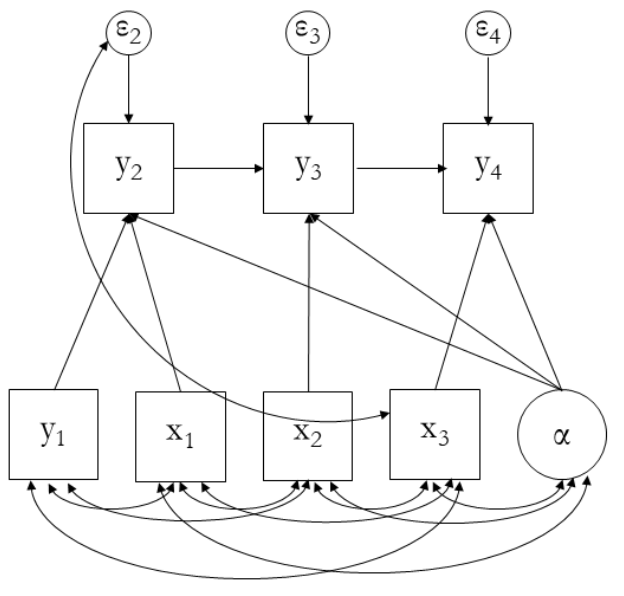
\includegraphics[width = 0.65\textwidth, height = 8cm]{Figures/Methodology/Sequential Ignorability.png}
    \label{fig:SeqIgnor}
    \caption*{\footnotesize{Note. All variables with dotted lines are assumed to be endogenous factors, capable of moderating the ODA effectiveness on health outcome.\\ Allison eta= al 2018.}}
\end{figure}

Therefore, to address both feedback and carryover effects, the autoregressive parameter (effect of $y_{it-1}$ on $y_{it}$) is controlled and  $x_{it}$ is treated predetermined or sequentially exogenous variable, as shown DPM Equation \ref{eq3}:

%given the intricate relationship between the variables of interest, this thesis employs a dynamic panel model alongside the fixed effect model. In the framework of a dynamic panel model (Figure \ref{fig:SeqIgnor}), Equation 4 can be expressed as:


\begin{equation}
    y_{it} = \delta y_{it-1} + \beta_{1} x_{it} + \theta z_{it} + \mu_i + \lambda_t + \epsilon_{it}
    \label{eq3}
\end{equation}

Here, $x_{it}$ being predetermined or sequentially exogenous implies that  $E[\epsilon_{it}|x_{it}, \mu_i] = 0$, for all $s \geq t$ \parencite{allison2017maximum}. In other words, $x_{it}$ is allowed to correlate with past error, but exogenous of current or future error \parencite{seddig2020maximum}. Notably, controlling for the autoregressive parameter (past outcome) as a predictor introduces additional endogeneity since both contemporaneous ($y_{it}$) and past ($y_{it-1}$) health outcomes are functions of and correlated with country characteristics, $\mu_i$ \parencite{shafa_assessment_2023, yogo_health_2015, nwude_official_2020}.

While scholars do not unanimously agree on a singular approach to address the endogeneity problem in dynamic panel analysis, econometricians commonly and popularly have employed instrumental variables (IV), particularly based on the first difference and system General Method of Moments (GMM) of Arellano-Bond (AB) approach for decades \parencite[see][]{arellano1991some, alonso1999symmetrically, allison2017maximum}. While the first difference AB method eliminates unit FE parameter, $\mu_i$ \parencite{arellano1991some}, system AB GMM uses both level and difference equations. However, recent studies based on simulations, have revealed significant weaknesses of IV-based and moment conditioning models. According to them, the major setbacks of GMM: are small-sample bias, particularly when panel wave, $t$, is small, and when autoregressive parameter, $\delta$, is close to 1.0 and sensitivity of the model to instruments \parencite{allison2017maximum, seddig2020maximum, becker2023many}.  Against this backdrop, the thesis adopts the Fixed Effect Cross-Lag Model (FE-CLM) of \textcite{allison2017maximum}, an approach based on maximum likelihood estimation of structural equation model (ML-SEM) specificy in Equation \ref{eq4}:
\begin{equation}
\begin{split}
    y_{it} = \delta y_{it-1} + \beta x_{it-1} + \theta z_{it} + \mu_i + \lambda_t + \epsilon_{it}\\
 x_{it} = \delta y_{it-1} + \beta x_{it-1} + \theta m_{it} + \rho_i + \tau_t + \epsilon_{it}
 \end{split}
    \label{eq4}
\end{equation}
The approach includes both the autoregressive ($\delta y_{it-1}$) and cross-lag ($\beta x_{it-1}$) parameters and employs a structural equation model with maximum likelihood estimation (ML-SEM) to analyze the causal predominance of lagged effect of $x$ and $y$ \parencite{seddig2020maximum}. The plausibility of this approach is that, first, it assumes multivariates normality of all endogenous variable $x_{it}$ and $y_{it}$, and even if the assumption is violated, ML-SEM produces a consistent and asymptotic estimate \parencite{allison2017maximum}. Furthermore, ML-SEM relaxes AB assumptions of temporal dynamics of the error variances at each time period. Finally, ML-SEM requires no specific instrumental variables  \parencite{allison2017maximum, becker2023many, moral2019dynamic}. 



%$t-j$, $j = 1, 2, 3...J$, refers to past or lagged values of the respective variables, $\delta$ for the vector of lagged health outcomes, and $\beta_{1}$ for lagged treatment (ODA allocation). In this model, as strict exogeneity fails ($E[\epsilon_{it}|x_{it}] \neq 0$), sequential ignorability allows us to assume that ODA is sequentially exogenous ($E[\epsilon_{it}|x_{it-j}] = 0$) \parencite[see][]{blackwell2018make, becker2023many, allison2017maximum}. 


%and the Fixed Effect Cross-Lag Model (FE-CLM) \parencite[see][]{allison2017maximum, becker2023many, moral2019dynamic}. Although the FE-CLM is considered to produce a superior and more consistent estimate, especially concerning the small sample bias of the AB method, it encounters significant convergence problems and computational difficulties \parencite{nino2022aid}. Consequently, this thesis adopts the system GMM proposed by \textcite{blundell1996econometric}. The AB GMM method utilizes an instrumental variable to address the endogeneity of the autoregressive parameter and country FE \parencite{nwude_official_2020, yogo_health_2015}. The system GMM represents an extension of the first difference GMM, offering higher asymptotic efficiency \parencite{nwude_official_2020}.


%$t-j$, $j = 1, 2, 3...J$, refers to past or lagged values of the respective variables, $\delta$ for the vector of lagged health outcomes, and $\beta_{1}$ for lagged treatment (ODA allocation). In this model, as strict exogeneity fails ($E[\epsilon_{it}|x_{it}] \neq 0$), sequential ignorability allows us to assume that ODA is sequentially exogenous ($E[\epsilon_{it}|x_{it-j}] = 0$) \parencite[see][]{blackwell2018make, becker2023many, allison2017maximum}.



\subsection*{4.3  Model Specifications and Hypotheses}
\addcontentsline{toc}{subsection}{4.3 Model Specifications and Hypotheses}
\subsubsection*{\quad 4.3.1 Hypothesis One}
The overarching objective of the thesis is to assess the impact of ODA on health outcomes. Given the multiple dimensions employed to measure health outcomes, the hypothesis for the research question is:

\begin{itemize}
    \item[i.] \(H_0\): \textit{ODA does not significantly affect at least one dimension of health outcomes in developing countries.}
\end{itemize}
To test this hypothesis, the thesis employs two approaches: first, the fixed effect cross-lag panel method with ML-SEM Equation in \ref{eq4} is re-specified in Equation \ref{eq5} below, with total ODA:   

%a basic sequential exogenous model with a two-way Fixed effect\footnote{Note: The first line of Equation \ref{eq5} is not a full Dynamic Panel Model (DPM) but a basic dynamic model to ensure that ODA is sequentially exogenous in predicting health outcomes without allowing the disturbance term \(\epsilon_{it}\) to correlate with ODA. The major element of a dynamic model is the autoregressive parameter \(\delta\) in Equation 5.}  and a dynamic model in eq. \ref{eq5}:

\begin{equation}
    HO_{it} = \delta HO_{it-1} + \beta_{1} ODA_{it-1} + \theta z_{it} + \mu_i + \epsilon_{it}
    \label{eq5}
\end{equation}

As robustness checks, a simple fixed effect is employed (without the autoregressive parameter, $\delta$) with social infrastructure ODA:
\begin{equation}
    HO_{it} = \beta_{1} ODA_{it-1} + \theta z_{it} + \mu_i + \lambda_t + \epsilon_{it}
    \label{eq6}
\end{equation}
%HO_{it} &= \beta_{1} ODA_{it-j} + \theta z_{it} + \mu_i + \lambda_t + \epsilon_{it} \\        

\subsubsection*{\quad 4.3.2 Hypothesis Two}

In furtherance of the main research question above, the thesis aims to assess whether the impact of ODA varies across regions, particularly SSA and non-SSA regions. 
\begin{itemize}
    \item[ii.] \(H_0\): \textit{The impact of ODA on health outcomes is not significantly different between SSA and non-SSA regions on at least one health dimension.}
\end{itemize}
The FE-CLMP, specified in Equation \ref{eq5}, is employed to test the hypothesis II, while controlling for interactions of respective regional dummy variable and total ODA, as shown in Equation 
\begin{equation}
    HO_{it} = \delta HO_{it-1} + \beta_{1} ODA_{it-1} + \beta_2 (SSA\times ODA_{it-1})  + \theta z_{it} + \mu_i + \lambda_t + \epsilon_{it}
    \label{eq7}
\end{equation}

%+ \beta_3 (Europe\times ODA_{it-1}) + \beta_4 (MENA\times ODA_{it-1}) + \beta_5 (LCA\times ODA_{it-1}) + \beta_6 (SCA\times ODA_{it-1})
%approach to capture the regional heterogeneity of SSA and non-SSA regions, with SSA countries taking value of 1, and non-SSA taking 0. The region dummy is then controlled and interacted with ODA, as shown in eq \ref{}


Here, $\beta_1$ (non-SSA), a vector of coefficients for non-SSA regions dummy interactions with ODA and $\beta_2$, a scalar coefficient for SSA region are the parameters of interest, representing the effect of ODA in SSA and non-SSA regions. A similar approach is replicated in the ordinary fixed effect model for robustness, albeit with social infrastructure ODA and without autoregressive parameter $\delta$. 

%This hypothesis will be tested by controlling for regions. The thesis classifies all developing countries in our analysis into six regions: MENA, SSA, Europe, EAP, LAC, SCA. 


\subsubsection*{\quad  4.3.3  Hypothesis Three:}
The thesis's third and final objective is to understand the mediating role of social protection in the impact of ODA on the health dimension. Thus, the hypothesis is that:

\begin{itemize}
    \item[iii.] \(H_0\): \textit{The indirect role of Social protection in the impact of ODA on health outcome is not statistically significant for at least one health dimension.}
\end{itemize}

While \textcite{yogo_health_2015} employed female education and health spending per capita, this thesis employs social protection as the potential mechanism. To model this relationship, the mediation causal approach with fixed effect is employed, discussed in \textcite{hayes2009beyond, hicks2011causal, becker2023many}. The path analysis is shown in the Directed Acyclic Graph (DAG) in Figure \ref{DAG-mediation} below:  
\begin{figure}[!ht]
\centering
\caption{Figure 4: Mediation Path analysis}
\resizebox{0.5\textwidth}{!}{%
\begin{circuitikz}
\tikzstyle{every node}=[font=\normalsize] % Adjust font size here

\draw (7.5,17) ellipse (1cm and 0.5cm) node {\normalsize ODA};
\draw (11.5,17) ellipse (1cm and 0.5cm) node {\normalsize HO};
\draw [->] (8.5,17) -- (10.5,17);
\node at (9.5,17.25) {c'};

\draw (9.5,19.5) ellipse (0.75cm and 0.5cm) node {\normalsize SP};
\draw [->] (7.75,17.5) -- (9.25,19);
\draw [->] (9.75,19) -- (11,17.5);
\node at (8.05,18.55) {a};
\node at (11.05,18.25) {b};

\draw [, dashed] (11.75,21.25) circle (0.5cm) node {\Large $\epsilon_1$};
\draw [, dashed] (14.5,18.25) circle (0.5cm) node {\Large $\epsilon_2$};
\draw [-Stealth, dashed] (11.25,20.75) -- (10.25,19.75);
\draw [-Stealth, dashed] (14,18) -- (12.5,17.25);
\end{circuitikz}
}%
\label{DAG-mediation}
\end{figure}

Path $c'$ represents the direct impact of ODA on health, path $a$ for ODA impact on social protection and path $b$ for the effect of social protection on health. The causal order is represented as follows: \(ODA_{it-4} \rightarrow SP_{it-3} \rightarrow HO_{it}\)\footnote{Note that, the causal order is a mere assumption, which may not necessarily be true \parencite[see][]{yogo_health_2015}.}. The total effect = \(c' + a\times b \), here, the main parameter of interest (social protection as mechanism) is the joint significance of $a \times b$. If they are both significant and the effect of ODA on health is reduced after controlling for Social protection, then social protection is a significant channel of ODA effect on health \parencite[see][]{becker2023many, yogo_health_2015}. 


\subsection*{4.4 Variable Selection, and Data Sources}
\addcontentsline{toc}{subsection}{4.4 Data, Variable Selection and Data Sources}
This thesis utilizes relevant secondary data for 144 developing countries, in Appendix C Table \ref{tab:country_info}, all of which are classified as ODA eligible by \textcite{oecd_Data_2023}. The dataset spans  22 years, between 2000 to 2021, a period chosen to align with the inception of the Sustainable Development Goals (SDG) in 2000. It's noteworthy that ODA data dates back further than SDG and the descriptive analysis of ODA in Chapter Two incorporated earlier data, starting from 1990. All study variables fall in three categories: the dependent variable (health outcomes); the main independent variable (ODA); and the control variables, also known as covariates. 

\subsubsection*{\quad 4.4.1 Dependent Variable: Health outcomes}
As outlined earlier, health is a complex and multidimensional concept. The literature review section unveils narrow indicators used to proxy health outcomes in prior studies (See Literature review section for details). For example, \textcite{nwude_official_2020} focused on life expectancy and under-5 mortality, while \textcite{odokonyero_impact_2018, bavinger_relationship_2017} used the burden of diseases, \textcite{doucouliagos_health_2021} utilized infant mortality, and \textcite{kavakli_us_2022} used family planning as a proxy for health outcomes. However, these indicators lack depth to adequately capture the diverse and nuanced nature of health across different regions. Furthermore, such narrow indicators may obscure the true impact of ODA.

Consequently, this thesis adopts a more holistic approach to measuring health. Specifically, Sustainable Development Goal (SDG) 3, on health and well-being, and SDG 2.3 on malnutrition are employed as proxies for health. These indicators provide a robust framework encompassing various health dimensions, facilitating an in-depth exploration of the impact of ODA on diverse aspects of health in developing countries. After the initial variable selection and correlation analysis, 26 health and malnutrition indicators, listed in Appendix A.2 Table \ref{Tab::health indicators}, were retained and subsequently used to construct six composite health dimensions. Appendix B Figure \ref{fig:combined_scat_plot}, illustrates the distribution of countries across respective health dimensions. See the discussion on respective health dimensions in Chapter Two and the procedure for the composite health dimensions in Appendix B.1.

The health dimensions constructed-reproductive risk and fatalities (RFTP), malnutrition, burden of infection and diseases (BID), health system capacity and responsiveness (HSCR), environmental death, and burden of mental problem (BMP)—each contribute to a comprehensive understanding of health outcomes. This approach elucidates the nuanced nature of health across world regions and the dynamic of ODA effectiveness on the diverse health dimensions. All health indicators were primarily sourced from the United Nations Sustainable Development Statistics (UNSDG) \parencite{unsdg_sustainable_2023}, the global database for data on SDG goals. To address the high levels of missing data for certain indicators in the UNSDG, the World Bank's World Development Indicators (WDI) database \parencite{wdi_world_2023} was utilized to supplement the dataset.

\subsubsection*{\quad 4.4.2 Independent Variables} 
\paragraph{\quad \quad \textit{4.4.2.1 Official Development Assistant (ODA)}}
\subparagraph{}
The main independent variable in this study is ODA, otherwise known as foreign aid, which is the financial and technical support provided by affluent countries for developmental purposes in developing nations. See Chapter Two for a discussion on ODA and its classification system in Appendix A.1 Figures \ref{fig:General ODA classification} and \ref{fig:Sector ODA classification}. While there is no consensus on the specific type of ODA to use when assessing its impact on health, many previous studies \parencite[e.g.,][]{nwude_official_2020, odokonyero_impact_2018} employed health ODA. Others, including \textcite{yan_mortality_2015, kavanagh_governance_2019, ali_foreign_2020, yogo_health_2015}, utilized the Global Health Fund, and \textcite{cassola_evaluating_2022} focused on research ODA. Additionally, \textcite{bavinger_relationship_2017} considered child health ODA, \textcite{marty_taking_2017} explored infrastructure and parasitic ODA, and \textcite{staicu2017study, akinola_foreign_2022} investigated total ODA. 

%Coefficients of ODA are expected to be negative for all health dimensions, but positive for health system capacity and responsiveness (HSCR)

As illustrated in Appendix A.1 Figure \ref{fig:Sector ODA classification}, health ODA constitutes only a small subsector of social infrastructure ODA. Additionally, other subsectors within social infrastructure ODA, apart from health, have elements of health. Therefore, this thesis, following preceding studies \textcite{williamson_foreign_2008, toseef_how_2019, doucouliagos_health_2021}, employed both total net and social infrastructure ODA. Net ODA is chosen over total disbursement to account for repayment over time. All ODA data were sourced from the OECD database \parencite{oecd_Data_2023}.

\paragraph{\quad \quad \textit{4.4.2.2 Social Protection}}
\subparagraph{}
In this study, social protection is hypothesized as a mediating channel through which ODA may impact health. While mediation analysis is relatively scarce in previous studies assessing the impact of ODA on health, studies, including \textcite[]{mahembe_foreign_2019, forte_impact_2023}, on ODA and social protection have rarely utilized explicit social protection indicators. Instead, many previous studies employed poverty and income per capita as proxies for social welfare. This choice is often attributed to the limited availability of panel data specifically focused on social protection, as highlighted by \textcite{nino-zarazua_aids_2023}. Similar to \textcite{nino-zarazua_aids_2023}, the thesis utilizes the coverage of all social protection as a proxy for social protection development in developing countries. The variable is measured as \% of the total population with access to any form of social protection and the data is sourced from the World Bank Aspire database \parencite{wdi_world_2023}. The coefficient of both ODA and social protection are expected to be negative for all health dimensions, except HSCR.  
 
\subsubsection*{\quad 4.4.3 Control Variables}
%\addcontentsline{toc}{subsubsection}{ 4.4.3 Control Variables}
The third classification of variables is covariates, also known as control variables. In this study, covariates are confounding factors affecting both ODA and health outcomes. They mitigate omitted variable bias (OVB) in the model and ensure baseline equivalence among study units. All control variables, except the Climate Risk Index (CRI) are sourced from the World Development Indicators \parencite{wdi_world_2023}. The following are the controlled variables considered in this study:

\begin{enumerate}[i]
    \item \textbf{GDP per Capita:} GDP per capita is fundamental to accounting for the initial level of economic development in a country. An increase in countries' GDP Per capita enhances their health outcome and reduces their likelihood of receiving ODA \parencite{oecd_ODA_Report_2023}. This variable, used in numerous reviewed studies \parencite[e.g.,][]{williamson_foreign_2008, nwude_impact_2023, toseef_how_2019}, is measured in 2017 constant price US dollars \textcite{wdi_world_2023}. The variable is logged in the model to address high skewness.
   % \item \textbf{Government Health Spending:} Domestic government health expenditure signifies the level of a country's commitment to its healthcare system. This spending not only influences the strength of the healthcare system but also impacts health outcomes, as used in previous studies \parencite{yan_mortality_2015, chung_economic_2022, mohamed_foreign_2017, akinola_foreign_2022}. The variable is measured as a percentage of total health spending in 2017 constant price \textcite{wdi_world_2023} and logged in the model.  
    \item \textbf{Domestic government health finance capacity:} The thesis employs both domestic government health spending per capita and stock of external debt, as a proxy for countries' public finance. While government health spending per capita signifies the level of a country's commitment to its healthcare system, \parencite[see][]{yan_mortality_2015, mohamed_foreign_2017, akinola_foreign_2022}, the external debt stock exerts downward pressure government's capacity to invest in the health system \parencite{kumar2010public, ogunjimi2019impact}. Surprisingly, prior studies did not control for government debt, despite its significant influence on public health finance in developing countries \parencite{kumar2010public}. Government spending per capita is measured in 2017 constant price, external debt is measured as per GNI \parencite{wdi_world_2023}. Both variables are logged to mitigate skewness.   
    
   % \item \textbf{Log(External Debt Stock):} A crucial factor influencing the public finance and investment capacity of many developing countries is public debt. In an IMF-published study, \textcite{kumar2010public} revealed a negative relationship trend between the external public debt-to-GDP ratio and economic growth. Specifically, a 10 percentage point rise in the initial debt-to-GDP ratio led to a 0.2 percentage point annual reduction in real per capita GDP growth \parencite{kumar2010public}. A more detailed negative impact of external debt is uncovered in a study by \textcite{ogunjimi2019impact} in Nigeria. Surprisingly, prior studies did not control for government debt, despite its significant influence on public health finance in developing countries. The variable is measured as a percentage of the country's GNI and sourced from the World Development Indicators \parencite{wdi_world_2023}. The thesis applies a logarithmic transformation to the variable to mitigate the impact of skewness caused by extreme debt-ridden countries.
    
    \item \textbf{Demographic factors:} Country size, proxy by population, and population density are crucial to countries' health outcomes. Countries with higher populations often strain healthcare systems. Population density may support healthcare infrastructure development, enhancing accessibility to medical facilities, but may also contribute to the spread of infectious diseases and inadequate sanitation, negatively affecting health. While  \textcite[e.g.,][]{staicu2017study, chung_economic_2022, yogo_health_2015, doucouliagos_health_2021} controlled for population as a proxy of country size, \textcite{doucouliagos_health_2021} employed both population and population density. Both variables are logged in the models.
 %   
  %  Higher populations often strain healthcare systems and correlate with increased health problems. This variable is measured in absolute values and sourced from the World Development Indicators \parencite{wdi_world_2023}. Despite its high correlation with other demographic variables, the population is retained due to its significance. The logarithmic transformation is applied to address skewness. Noteworthy, this variable exhibits a positive effect on all health dimensions, with a specific positive impact on HSCR.
   % \item \textbf{Log(Population Density):} Another vital social demographic factor influencing health is population density, in accordance with previous studies \parencite{toseef_how_2019, doucouliagos_health_2021}. The thesis controls for population density, measured as people per square kilometer of land area, with data sourced from the World Development Indicators \parencite{wdi_world_2023}. To address skewness, a log transformation is applied.
    %Higher population density can have a dual impact: it may support healthcare infrastructure development, enhancing accessibility to medical facilities, but it can also contribute to the spread of infectious diseases and inadequate sanitation, negatively affecting health. Consequently, the thesis anticipates a negative association of population density with all health dimensions, while expecting a positive effect on health system capacity and responsiveness.
    
    \item \textbf{Infrastructure development:} The level of infrastructure development plays a crucial role in the overall health and well-being of citizens. While \textcite{doucouliagos_health_2021, yogo_health_2015} controlled for sanitation and water access, \textcite{odokonyero_impact_2018, yan_mortality_2015, williamson_foreign_2008} employed urbanization to measure infrastructure development. As utilized by \textcite{toseef_how_2019} and due to the high correlation of electricity access with various development indicators, including education, sanitation and water access, HDI etc, the thesis employs electricity access as a proxy of the infrastructure development level of countries.  Electricity access is measured as the percentage of the population with access to electricity \textcite{wdi_world_2023}. 
    
    \item \textbf{Alternative foreign inflow:} Foreign Direct Investment (FDI) and remittance are crucial alternative foreign inflows in developing countries \parencite{scott_lessons_2020}, capable of bolstering investment capital and strengthening health systems and outcomes. The nature of impact of all foreign inflows depends on the recipients of those flows: while remittance flows to households \parencite[see][]{obi2020does, gamlen2014new, de2009remittances}, FDI encourages flow technology \parencite{chung_economic_2022} and ODA flow more to the government. Regardless, all foreign inflows, regardless of their nature, have an enormous impact on health outcomes and the well-being of developing countries, thus making FDI and remittances crucial in the thesis models.   
    
    %While \textcite{yogo_health_2015} controlled for remittance per capita, remittances typically don't directly contribute to government funds, limiting their impact on public health investment and overall national development \parencite[see][]{obi2020does, gamlen2014new, de2009remittances}. In alignment with \textcite{chung_economic_2022}, this thesis opts for FDI as an alternative foreign financial flow. The variable is measured as net inflows as a percentage of GDP, with data sourced from the World Development Indicators \parencite{wdi_world_2023}.
    
    \item \textbf{Climate Risk Index Score:} The Climate Risk Index (CRI) Score ranks countries and regions based on their vulnerability to the impacts of climate change, particularly extreme weather events like storms, heatwaves, and floods \parencite{eckstein2021global}. The escalating impact of climate change on global health cannot be overstated. While \textcite{nwude_official_2020} controlled for CO$_2$ emissions, the thesis contends that the impact of climate change on the health of developing countries' populations is not necessarily proportional to their emissions. Hence, the thesis opts for the CRI Score, which reflects the vulnerability and exposure of developing countries to various climate impacts, likely affecting population health. The CRI Score, compiled by German Watch, ranges from 2 to 166 and is sourced from the most recent version in 2021 \parencite{eckstein2021global}. 
    
    %\item \textbf{Log(Trade per GNI):} Trade is a fundamental factor influencing the economic development, health, and overall well-being of a country. Nations with higher trade tend to exhibit positive economic and health outcomes \parencite[see][]{makki2004impact, pavcnik2017impact}. Previous studies incorporated trade in various forms, such as export value in \textcite{chung_economic_2022} and net trade values in \textcite{forte_impact_2023, shafiullah_foreign_2011}, as a proxy for countries' trade openness. In a similar vein, this thesis controls for countries' level of trade, measured as a percentage of GDP. The variable undergoes a log transformation, and raw data is sourced from the World Development Indicators \parencite{wdi_world_2023}. Trade is anticipated to have a negative effect on all health dimensions but a positive impact on health system capacity and responsiveness.
    
    \item \textbf{Quality of governance:} The impact of institutional/governance quality continues to be debated \parencite[e.g.][]{doucouliagos_health_2021, williamson_foreign_2008}. Previous studies have employed various governance proxies, such as control of corruption, Fraser freedom index, civil conflict, political regimes, and democracy index sourced from the World Development Indicators \parencite{shafiullah_foreign_2011, muhammad_health_2021, toseef_how_2019, williamson_foreign_2008, kavakli_us_2022, yogo_health_2015}. In this thesis, governance quality is proxied by the general Governance Index, which allows inter-country comparisons across six crucial governance dimensions: voice and accountability, political stability and absence of violence, government effectiveness, regulatory quality, rule of law, and control of corruption \parencite[see][for detailed description of the index]{handoyo2023worldwide, wdi_world_2023}.
\end{enumerate}









     
       






 
 



\subsection*{4.5 Data Analysis Tools}
\addcontentsline{toc}{subsection}{4.5 Data Analysis Tools}
The thesis employs R-programming for data analysis. Key packages utilized include SDG and WDI,  used for loading data from the World Bank and UN statistics. Tidyverse was used for all data transformation and plots. MisForest was employed for imputing missing values; Plm and DPM for econometric analysis and hypothesis testing; LmTest for robust standard error estimation due to heteroscedasticity. Also, Groundhog was used to keep packages updated to ensure the reproducibility of findings. All code scripts for the data analysis are submitted alongside the thesis. 






%\subsubsection*{General Panel Tests for Model Specification}

%Multicollinearity test, Poolability/Panel Test, Homoscedasticity test, Serial Correlation test, and stationarity test.

%(individual time varying characteristics varies across units and time dimensions which is the error term in FE)

\section*{\centering Chapter Five}
\section*{\centering Presentation of Findings}
%\addcontentsline{toc}{section}{Chapter Five}
\addcontentsline{toc}{section}{Chapter Five: Presentation of Findings}
%\subsection*{5.0 \quad Introduction}

The chapter begins with a statistical summary of variables presented in Appendix Table \ref{Tab::Stat_summary} and relevant econometric tests in Appendix Tables \ref{tab:VIF_reslts}, \ref{Tab::UnitFE_Test}, \ref{Tab::TimeFE_test}, \ref{Tab::Heteroskedict}, and \ref{Tab::Serial_corr_Test}. Following this, the chapter presents all models and their respective interpretations. The primary independent variables in the models are total net and social infrastructure Official Development Assistance (ODA), both of which are log-transformed. The main outcome variable is health outcome, proxied by six composite health dimensions: Reproductive Fatality and Teen Pregnancy (RFTP), Burden of Infection and Diseases (BID), Malnutrition, Environmental Death, Burden of Mental Problems (BMP), and Health System Capacity and Responsiveness (HSCR). 
%As outlined in the methodology section, all coefficients are interpreted as the Average Causal Response to Treatment (ACRT). This represents the average marginal effect of ODA allocation on health outcomes among the treated (the actual recipients of ODA) over the specified period in the data   

%\subsubsection*{5.1 \quad Preliminary Econometrics Tests}
%Appendix C Table \ref{tab:VIF_reslts}, \ref{Tab::UnitFE_Test}, \ref{Tab::TimeFE_test}, \ref{Tab::Heteroskedict} and \ref{Tab::Serial_corr_Test} contains the five major panel tests crucial for justifying the chosen estimation approach. These tests include the multicollinearity test for control variables, the Lagrange Multiplier panel effect test guiding the selection of fixed effect, the Breusch-Pagan test examining the heteroscedasticity of errors, and BreuschGodfrey/Wooldridge Test for Serial Correlation. 
%As shown in the variance inflator factor (VIF) in Appendix C Table \ref{tab:VIF_reslts}, the coefficients of all control variables are below 5, which is the rule of thumb in econometrics for absence of multicolinearity \parencite{baltagi2008econometric}. The relationship between the variables can be viewed in the Appendix Figure \ref{fig:Correlation_Matrix_Graph}. Furthermore, in panel model, it is essential to test to for presence of unit and time fixed effect to determine whether pooled Ordinary Least Square (OLS), using langrange multiplier test. The result of unit fixed effect and time fixed effect are shown in Appedix Table \ref{Tab::UnitFE_Test} and \ref{Tab::TimeFE_test} respectively. Accordingly, all the p-values of various models in Table \ref{Tab::UnitFE_Test} are below 5\% against the null hypothesis that there is no unit (country in this case) effect, thus, pooled OLS will be biased and fixed effect model is appropriate. Surprisingly, as shown in Appendix Table \ref{Tab::TimeFE_test}, only the model on burden of mental problem has p-value below 5\%, showing no substantial concern for time effect. Based on the two Lagrange panel tests, a unit FE is combined with a time trend as control variable.   


%Moreover, an essential regression assumption to obtain an unbiased estimate is that observations are identically and independently distributed (i.i.d), which is essential for homoskedasticity of errors. Violation of this assumption does not affect the estimate, but the standard error will be inaccurate \parencite[see][]{doucouliagos_health_2021, williamson_foreign_2008, nwude_official_2020}. Based on the Breusch-Pagan error distribution test in Appendix C Table \ref{Tab::Heteroskedict}, the p-value is below 5\% against the null hypothesis that errors are homoskedastic. Thus, there is presence of heteroskedasticity of the error terms. Similar problem is observed is observed in the BreuschGodfrey/Wooldridge Test in Appendix C Table \ref{Tab::Serial_corr_Test}, which shows the presence of temporal dependency, also known as serial correlation. To correct for all these, the thesis consistently reports heteroskedasticity-autocorrelation (HAC) corrected standard errors in all estimated models.


\subsubsection*{5.1 Preliminary Econometrics Tests}
\addcontentsline{toc}{subsection}{5.1 Preliminary Econometrics Tests}

Appendix C includes the results of five major panel tests crucial for justifying the chosen estimation approach (see Table \ref{tab:VIF_reslts}, \ref{Tab::UnitFE_Test}, \ref{Tab::TimeFE_test}, \ref{Tab::Heteroskedict}, and \ref{Tab::Serial_corr_Test}). These tests cover aspects such as multicollinearity, selection of fixed effects, heteroscedasticity of errors, and serial correlation. The variance inflation factor (VIF) in Appendix Table \ref{tab:VIF_reslts} indicates that the coefficients of all control variables are below 5, adhering to the rule of thumb in econometrics for the absence of multicollinearity \parencite{baltagi2008econometric}. The relationship between variables is can be visualized in Appendix Figure \ref{fig:Correlation_Matrix_Graph}.

In panel models, testing for the presence of unit and time fixed effects is essential, to determine the appropriateness of pooled, random or fixed effect. The results in Table \ref{Tab::UnitFE_Test} and \ref{Tab::TimeFE_test} reveal that all p-values for various models against the null hypothesis of no unit (country) effect are below 5\%, suggesting that pooled Ordinary Least Squares (OLS) would be biased, and a fixed-effect model is appropriate. Surprisingly, only the model on the burden of mental problems (BMP) in Appendix Table \ref{Tab::TimeFE_test} has a p-value below 5\%, indicating no substantial concern for time effects. Based on these findings, a unit fixed effect is combined with a time trend as a control variable for all models.

Additionally, to obtain unbiased estimates, an essential regression assumption is that observations are identically and independently distributed (i.i.d), crucial for the homoskedasticity of errors or $cov(\epsilon, x) = 0$. The Breusch-Pagan error distribution test in Appendix Table \ref{Tab::Heteroskedict} shows a p-value below 5\% across all health dimensions, indicating the presence of heteroskedasticity. While violation of this assumption does not affect the estimate, the standard error will be inaccurate \parencite[see][]{doucouliagos_health_2021, williamson_foreign_2008, nwude_official_2020}. A similar issue is observed in the Breusch-Godfrey/Wooldridge Test in Table \ref{Tab::Serial_corr_Test}, indicating temporal dependency, otherwise known as serial correlation. To address these concerns, the thesis consistently reports heteroskedasticity-autocorrelation (HAC) corrected standard errors in all estimated models.




\subsection*{5.2 Result Presentation and Interpretation}
\addcontentsline{toc}{subsection}{5.2 Result Presentation and Interpretation}
The result section is organized according to the research questions and respective hypotheses. The thesis draws evidence using four panel estimation approaches: unit fixed effect with time trend as a control variable, Fixed-Effect Cross-Lag Panel Model (FE-CLPM), and local projection, and mediation path analysis with bootstrapping.  While the fixed effect model serves as a benchmark for comparison against other models, the FE-CLPM approach is a dynamic panel model using Maximum Likelihood Structural Equation Model (ML-SEM) to address reverse causality. Notably, population and population density control variables were excluded from all FE-CLPM models due to convergence problems. Furthermore, the local projection approach is used as an alternative dynamic approach to explore the temporal dynamics of ODA across various health dimensions. The mediation path analysis is mainly used to test the indirect role of social protection in the impact of ODA on various health dimensions. 


In each result table, there are six models, each of which represents the six health dimensions under study. Due to the enormous estimated models in the local projection, only the coefficients of interest (ODA) for respective health dimensions are plotted. All models across methods are estimated with 22 years data (2000 to 2021) mean aggregated into five periods, except for local projection and mediation path analysis, where year wave data is employed, for 144 countries across six regions (see Table \ref{tab:country_info} for list of countries and regions).  As implemented in previous studies \parencite[i.e.][]{yogo_health_2015, williamson_foreign_2008}, data aggregation helps in addressing noise, preventing serial correlation and non-stationarity in the data. In all cases, the thesis reported heteroskedasticity-autocorrelation (HAC) corrected standard errors due to heteroskedasticity of errors. Moreover, only the coefficient of key variable (ODA and social protection) on various health dimensions are interpreted in all models. 


%Different panel econometric approaches are employed to draw evidence: unit fixed effect with a time trend as a control variable, fixed-effect cross-lag dynamic panel model (FE-CLDM), and local projection. While the fixed-effect model serves as a benchmark for comparison, the FE-CLDM and local projection methods address endogeneity concerns using dynamic panel methodology. Each result table encompasses six models, representing the six health dimensions under study. Due to the complexity of the estimated models in the local projection, only the coefficients of ODA for respective health dimensions are plotted. All models, across methods, are estimated using 22 years of data (2000 to 2021) mean-aggregated into five periods, except for local projection, where year-wave data is employed. The study covers 144 countries across six regions (refer to Table \ref{tab:country_info} for the list of countries and regions). Data aggregation, as implemented in previous studies (Yogo et al., 2015; Williamson, 2008), aids in addressing noise and preventing serial correlation in the data. Heteroskedasticity-autocorrelation (HAC) corrected standard errors are consistently reported in all cases. In the result presentations, the focus is solely on interpreting the coefficient of key variables (ODA and social protection) relevant to the research questions across various health dimensions. The three main study hypotheses are:


%For the main research question, three distinct econometric methods were employed: the unit fixed effect model, dynamic panel model with system GMM, and local projection method, all with a time trend as a control variable. For the second research question focusing on regional heterogeneity of effect, the thesis utilized the fixed effect model while controlling for a regional dummy specifically for Sub-Saharan Africa. For the final research question on the mediating role of social protection, mediation analysis is conducted, and only the coefficients of interest are reported. For robustness checks, the main predictor variable is switched from total ODA to Social infrastructure ODA, both for the primary and regional variation research questions. %The thesis begins the result presentation from the research one, primarily focusing on the impact of ODA on health.  

\subsubsection*{\quad 5.2.1  Impact of ODA on Health Outcome} 
This main overarching research question, aims to test whether the coefficient of ODA is significant on at least one of the six health dimensions. The hypothesis is that:
 \begin{enumerate}[i]
    \item \textit{$H_0$: ODA does not significantly affect at least one dimension of health outcomes in developing countries.}
\end{enumerate}
The followings are the results:  
\subsubsection*{\quad \quad \textit{5.2.1.1 Unit Fixed Model Model with Time Trend as Control}}
Table \ref{table:FE_RQ1} presents the unit Fixed Effect (FE) linear-log model, for the six health dimensions with a one-period lag of ODA. All coefficients of ODA across health dimensions shows expected direction of effect except health system capacity (HSCR). Specifically, a 1\% increase in one period lagged ODA, on average, reduces reproductive fatalities and teen pregnancy (RFTP) by 0.016, burden of infection and diseases (BID) by 0.008, environmental death by 0.018, malnutrition by 0.003 and burden of mental problems (BMP) by 0.016 standard deviations, respectively. Albeit, ODA is only weakly significant for reproductive fatality at 10\% p-value, while it has negative negative impact on health system capacity, with effect estimates of -0.011 standard deviations. 
\renewcommand{\arraystretch}{0.35} 
%\afterpage{
\begin{longtable}{@{\extracolsep{-3pt}}lcccccc} 
\caption{Unit Fixed Effect with Time Trend as Control (linear-log model)}
\\[-0.9ex]\hline 
\hline \\[-0.9ex] 
 & \multicolumn{6}{c}{\textit{Dependent variables:}} \\ 
\cline{2-7} 
\\[-0.9ex] 
 & Reprod. & Infect. \& & Mental & Malnutr- & Envir.  & Health\\
& Fatality & Diseases & Burden & tion & Death & Capacity  \\
\\[-1.8ex] & (1) & (2) & (3) & (4) & (5) & (6)\\ 
\hline \\[-0.9ex]
log(ODA)$_{t-1}$       & $-0.016^{*}$   & $-0.008$       & $-0.016$       & $-0.003$       & $-0.018$       & $-0.011$      \\
                    & $(0.007)$      & $(0.005)$      & $(0.013)$      & $(0.007)$      & $(0.017)$      & $(0.009)$     \\
                    &&&&&&\\
Elect\_Access                  & $-0.007^{***}$ & $-0.005^{**}$  & $-0.002$       & $-0.002$       & $-0.001$       & $0.005^{***}$ \\
                    & $(0.002)$      & $(0.002)$      & $(0.002)$      & $(0.002)$      & $(0.001)$      & $(0.001)$     \\
                    &&&&&&\\
log(GDP\_PerCap)       & $-0.061$       & $-0.118^{*}$   & $0.027$        & $-0.495^{***}$ & $-0.233^{***}$ & $0.336^{***}$ \\
                    & $(0.083)$      & $(0.054)$      & $(0.076)$      & $(0.107)$      & $(0.066)$      & $(0.056)$     \\
                    &&&&&&\\
Climate\_Risk\_Index          & $0.001$        & $0.000$        & $0.001$        & $-0.000$       & $0.001$        & $-0.001^{*}$  \\
                    & $(0.000)$      & $(0.000)$      & $(0.001)$      & $(0.000)$      & $(0.000)$      & $(0.001)$     \\
                    &&&&&&\\
log(Remittance)     & $-0.003$       & $0.002$        & $-0.003$       & $-0.005$       & $-0.005$       & $0.007$       \\
                    & $(0.003)$      & $(0.002)$      & $(0.003)$      & $(0.006)$      & $(0.004)$      & $(0.004)$     \\
                    &&&&&&\\
log(Population)            & $-1.080^{***}$ & $-0.956^{***}$ & $-0.090$       & $-0.591^{*}$   & $-0.154$       & $-0.293$      \\
                    & $(0.294)$      & $(0.257)$      & $(0.559)$      & $(0.300)$      & $(0.392)$      & $(0.184)$     \\
                    &&&&&&\\
log(Pop\_Density)      & $0.312$        & $0.494^{*}$    & $0.166$        & $-0.132$       & $-0.094$       & $0.501^{***}$ \\
                    & $(0.217)$      & $(0.246)$      & $(0.552)$      & $(0.235)$      & $(0.345)$      & $(0.135)$     \\
                    &&&&&&\\
log(Hlth\_Spnd\_PerCap)  & $0.037$        & $0.031$        & $0.100^{*}$    & $-0.074$       & $0.075$        & $0.075^{*}$   \\
                    & $(0.046)$      & $(0.045)$      & $(0.047)$      & $(0.070)$      & $(0.055)$      & $(0.038)$     \\
                    &&&&&&\\
Governance\_Index                 & $-0.052$       & $-0.025$       & $-0.031$       & $-0.165^{***}$ & $-0.074$       & $0.067$       \\
                    & $(0.047)$      & $(0.043)$      & $(0.053)$      & $(0.049)$      & $(0.049)$      & $(0.048)$     \\
                    &&&&&&\\
log(External\_Debt) & $0.024$        & $0.003$        & $0.006$        & $0.035$        & $-0.026$       & $-0.036^{*}$  \\
                    & $(0.017)$      & $(0.015)$      & $(0.014)$      & $(0.018)$      & $(0.018)$      & $(0.016)$     \\
                    &&&&&&\\
Time\_Trend           & $-0.042^{***}$ & $-0.016^{*}$   & $-0.053^{***}$ & $0.006$        & $-0.055^{***}$ & $0.024^{*}$   \\
                    & $(0.011)$      & $(0.008)$      & $(0.015)$      & $(0.012)$      & $(0.014)$      & $(0.010)$     \\
\hline \\[-0.9ex]
Num.Obs. & \num{576} & \num{576} & \num{576} & \num{576} & \num{576} & \num{576}\\
R2 & \num{0.768} & \num{0.566} & \num{0.258} & \num{0.621} & \num{0.564} & \num{0.581}\\
R2 Adj. & \num{0.683} & \num{0.407} & \num{-0.014} & \num{0.482} & \num{0.405} & \num{0.427}\\
AIC & \num{-1162.8} & \num{-1239.9} & \num{-872.3} & \num{-1005.1} & \num{-1006.8} & \num{-1023.8}\\
BIC & \num{-1110.6} & \num{-1187.6} & \num{-820.0} & \num{-952.8} & \num{-954.5} & \num{-971.5}\\
RMSE & \num{0.09} & \num{0.08} & \num{0.11} & \num{0.10} & \num{0.10} & \num{0.10}\\
\hline 
\caption*{\scriptsize{Note: The fixed Model model does not contain the autoregressive parameter due to the endogeneity problem discussed in Chapter Four. This makes FE models non-dynamic. We estimated a series of this model, switching control variables. When Foreign direct investment is controlled alongside remittance, the model fitness performs poorly. However, using only remittance improved the model. Also trade is excluded due to redundancy. Author's computation with data from \textcite{wdi_world_2023, unsdg_sustainable_2023}. $^{***}p<0.001$; $^{**}p<0.05$; $^{*}p<0.1$}}
\label{table:FE_RQ1}
\end{longtable}





%Additionally, Government health spending per total health spending, although negative for other health dimensions, is statistically significant and positive for health system capacity and mental burden. GDP per capita exhibits the expected direction of effect for all health dimensions and is statistically significant. Another notable finding is the impact of External debt on various health dimensions. Holding all else constant, external debt stock, on average, amplifies all health problems and negatively affects health system capacity and responsiveness. Lastly, governance is only statistically significant and negative for malnutrition, while displaying an insignificant effect direction for other health dimensions except infections and diseases.
\subsubsection*{\quad \quad \textit{5.2.1.2 Fixed Effect Cross-Lag Panel Model (FE-CLPM)}}
Table \ref{table:DPM_RQ1} shows the results of the linear-log model estimated with the Fixed Effect Cross-Lag Panel Model (FE-CLPM). The model incorporates the autoregressive parameters (impact of previous health outcome on current health outcome) and fewer control variables, excluding population and population density. Similar to the unit fixed effect model above, all coefficients of the one-period lagged ODA exhibit the anticipated direction of effects (negative) for all health dimensions, except healthcare capacity and responsiveness (HSCR). Specifically, a one-period lagged ODA, on average, reduces reproductive fatality (RFTP) by 0.041, burden of infection and diseases (BID) by 0.030, malnutrition by 0.042, and environmental death by 0.035 and burden of mental problems (BMP) by 0.066 standard deviations respectively. Notably, and unlike the unit fixed effect model, the impact of ODA is now highly significant for RFTP at 1\% and mildly significant for BID, malnutrition at 5\%, and environmental death at 10\% p\_value. 
\renewcommand{\arraystretch}{0.4} 
  
\begin{longtable}{@{\extracolsep{-3pt}}lcccccc} 
\caption{Fixed Effect Cross-Lag Dynamic Panel Model (linear-log model with aggregated data)} 
\\[-1.8ex]\hline 
\hline \\[-1ex] 
 & \multicolumn{6}{c}{\textit{Dependent variables:}} \\ 
\cline{2-7} 
\\[-1ex] 
 & Reprod. & Infect. \& & Mental & Malnutr- & Envir.  & Health\\
& Fatality & Diseases & Burden & tion & Death & Capacity  \\
\\[-1ex] & (1) & (2) & (3) & (4) & (5) & (6)\\ 
\hline \\[-1ex]

log(ODA)$_{t-1}$                   & $-0.041^{***}$ & $-0.030^{**}$ & $-0.066$      & $-0.042^{**}$ & $-0.035^{*}$  & $-0.015$      \\
                                & $(0.010)$      & $(0.010)$     & $(0.040)$     & $(0.014)$     & $(0.014)$     & $(0.009)$     \\
        &&&&&&\\
Elect\_Access                              & $0.000$        & $-0.001$      & $-0.003$      & $0.001$       & $0.000$       & $0.003^{***}$ \\
                                & $(0.001)$      & $(0.001)$     & $(0.002)$     & $(0.001)$     & $(0.001)$     & $(0.001)$     \\
                                &&&&&&\\
log(GDP\_PerCap)                   & $0.062$        & $-0.010$      & $0.023$       & $-0.024$      & $0.007$       & $0.208^{***}$ \\
                                & $(0.042)$      & $(0.062)$     & $(0.072)$     & $(0.097)$     & $(0.060)$     & $(0.045)$     \\
                                &&&&&&\\
Climate\_Risk\_Index                      & $-0.000$       & $-0.000$      & $-0.000$      & $-0.001$      & $0.001^{*}$   & $-0.001$      \\
                                & $(0.000)$      & $(0.000)$     & $(0.001)$     & $(0.000)$     & $(0.000)$     & $(0.000)$     \\
                                &&&&&&\\
log(Remittance)                 & $0.000$        & $0.001$       & $0.004$       & $-0.006^{*}$  & $0.001$       & $0.005^{**}$  \\
                                & $(0.002)$      & $(0.003)$     & $(0.005)$     & $(0.003)$     & $(0.002)$     & $(0.002)$     \\
                                &&&&&&\\
log(Hlth\_Spnd\_PerCap)             & $-0.012$       & $-0.077$      & $-0.043$      & $0.000$       & $0.076$       & $0.094^{**}$  \\
                                & $(0.023)$      & $(0.047)$     & $(0.082)$     & $(0.059)$     & $(0.046)$     & $(0.031)$     \\
                                &&&&&&\\
Governance\_Index                             & $-0.053$       & $-0.001$      & $-0.001$      & $-0.063$      & $-0.043$      & $0.042$       \\
                                & $(0.031)$      & $(0.036)$     & $(0.056)$     & $(0.047)$     & $(0.045)$     & $(0.035)$     \\
                                &&&&&&\\
log(External\_Debt)             & $0.013$        & $-0.011$      & $-0.061^{*}$  & $0.048^{*}$   & $0.010$       & $-0.021$      \\
                                & $(0.015)$      & $(0.016)$     & $(0.024)$     & $(0.021)$     & $(0.017)$     & $(0.014)$     \\
                                &&&&&&\\
Reprod\_Fatality$_{(t - 1)}$    & $0.768^{***}$  &               &               &               &               &               \\
                                & $(0.035)$      &               &               &               &               &               \\
                                &&&&&&\\
Infection\_Diseas$_{(t - 1)}$   &                & $1.138^{***}$ &               &               &               &               \\
                                &                & $(0.068)$     &               &               &               &               \\
                                &&&&&&\\
Mental\_Burden$_{(t - 1)}$   &                &               & $1.240^{***}$ &               &               &               \\
                                &                &               & $(0.099)$     &               &               &               \\
                                &&&&&&\\
Malnutrition$_{(t - 1)}$   &                &               &               & $0.896^{***}$ &               &               \\
                                &                &               &               & $(0.097)$     &               &               \\
                                &&&&&&\\
Environ\_Death$_{(t - 1)}$ &                &               &               &               & $0.825^{***}$ &               \\
                                &                &               &               &               & $(0.111)$     &               \\
                                &&&&&&\\
HealthSys\_Capacity$_{(t - 1)}$     &                &               &               &               &               & $0.512^{***}$ \\
                                &                &               &               &               &               & $(0.074)$     \\
                                
\hline \\[-1.1ex]
DF                              & $89.000$       & $89.000$      & $89.000$      & $89.000$      & $89.000$      & $89.000$      \\
Chi-Square ($\chi^2$)                           & $257.574$      & $212.063$     & $249.795$     & $286.456$     & $173.344$     & $150.279$     \\
Observations (N)                               & $144.000$      & $144.000$     & $144.000$     & $144.000$     & $144.000$     & $144.000$     \\
RMSEA                           & $0.115$        & $0.098$       & $0.112$       & $0.124$       & $0.081$       & $0.069$       \\
RMSEA  90\% CI Lower  & $0.098$       & $0.081$       & $0.096$       & $0.108$       & $0.063$       & $0.049$       \\
RMSEA  90\% CI Upper                  & $0.131$        & $0.115$       & $0.129$       & $0.140$       & $0.099$       & $0.088$       \\
p(RMSEA $<$ 0.05)                    & $0.000$        & $0.000$       & $0.000$       & $0.000$       & $0.003$       & $0.055$       \\
SRMR                            & $0.012$        & $0.015$       & $0.016$       & $0.013$       & $0.010$       & $0.006$       \\
\hline
\caption*{\scriptsize{Note: This table presents is a linear-log FE-CLPM model, with all control variables except population and population density, excluded due to convergence problem. The parameters in diagonal are the autoregressive parameters, which makes the model dynamic. Author's computation with data \textcite{wdi_world_2023, unsdg_sustainable_2023}. $^{*}$p$<$0.1; $^{**}$p$<$0.05; $^{***}$p$<$0.01}}
\label{table:DPM_RQ1}
\end{longtable}

%
Furthermore, the Table \ref{table:DPM_RQ1_Log} shows the log-log (elasticity) version of FE-CLDM, the result is stable across all the health dimensions, with some of the mentioned health dimensions becoming even more significant. It is noteworthy that the coefficients of all autoregressive parameters are highly significant, indicating the strong influence of the initial health situation on contemporaneous health and the appropriateness of the dynamic model approach for this study. 
%list(RFTP_Region_DPM, BID_Region_dpm, BMP_Region_dpm, Malnuti_Region_dpm, EnvDeath_Region_dpm, HSCR_Region_dpm)
\renewcommand{\arraystretch}{0.4} % 
\begin{longtable}{@{\extracolsep{-3pt}}lcccccc} 
 \caption{Fixed Effect Cross-Lag Dynamic Panel Model (log-log model with aggregated data)} 
\\[-1.8ex]\hline 
\hline \\[-1ex] 
 & \multicolumn{6}{c}{\textit{Dependent variables:}} \\ 
\cline{2-7} 
\\[-1ex] 
 & Reprod. & Infect. \& & Mental & Malnutr- & Envir.  & Health\\
& Fatality & Diseases & Burden & tion & Death & Capacity  \\
\\[-1ex] 
& (1) & (2) & (3) & (4) & (5) & (6)\\ 
\hline \\[-1ex]
log(ODA)$_{t-1}$             & $-0.014^{**}$ & $-0.029^{***}$ & $-0.030^{**}$ & $-0.020^{**}$ & $-0.012$      & $-0.001$      \\
                          & $(0.005)$     & $(0.009)$      & $(0.011)$     & $(0.008)$     & $(0.008)$     & $(0.004)$     \\
                          &&&&&&\\
%ae                        & $-0.000$      & $-0.001$       & $-0.001$      & $-0.000$      & $-0.000$      & $0.001$       \\
 %                         & $(0.000)$     & $(0.001)$      & $(0.001)$     & $(0.001)$     & $(0.001)$     & $(0.001)$     \\
%log\_GDP\_Cap             & $0.016$       & $-0.023$       & $-0.003$      & $0.037$       & $0.010$       & $0.076^{**}$  \\
%                          & $(0.023)$     & $(0.051)$      & $(0.042)$     & $(0.043)$     & $(0.034)$     & $(0.026)$     \\
%cri\_score                & $-0.000$      & $0.000$        & $-0.000$      & $-0.000$      & $0.001^{*}$   & $-0.000$      \\
%                          & $(0.000)$     & $(0.000)$      & $(0.000)$     & $(0.000)$     & $(0.000)$     & $(0.000)$     \\
%log\_remittance           & $0.000$       & $0.001$        & $0.004$       & $-0.001$      & $0.001$       & $0.002^{*}$   \\
%                          & $(0.001)$     & $(0.003)$      & $(0.003)$     & $(0.001)$     & $(0.001)$     & $(0.001)$     \\
%log\_hlth\_Per\_Cap       & $0.001$       & $-0.042$       & $-0.003$      & $0.012$       & $0.030$       & $0.034^{*}$   \\
%                          & $(0.013)$     & $(0.039)$      & $(0.040)$     & $(0.032)$     & $(0.025)$     & $(0.016)$     \\
%gov                       & $-0.038$      & $-0.020$       & $0.003$       & $-0.025$      & $-0.029$      & $0.017$       \\
%                          & $(0.020)$     & $(0.038)$      & $(0.028)$     & $(0.027)$     & $(0.027)$     & $(0.015)$     \\
%log\_External\_debt       & $0.005$       & $-0.011$       & $-0.025$      & $0.032^{**}$  & $-0.002$      & $-0.007$      \\
%                          & $(0.008)$     & $(0.014)$      & $(0.014)$     & $(0.011)$     & $(0.009)$     & $(0.008)$     \\
log(Reprod\_Fatality$_{(t - 1)}$)     & $0.801^{***}$ &                &               &               &               &               \\
                          & $(0.050)$     &                &               &               &               &               \\
                          &&&&&&\\
log(Infection\_Diseas$_{(t - 1)}$)      &               & $1.242^{***}$  &               &               &               &               \\
                          &               & $(0.074)$      &               &               &               &               \\
                          &&&&&&\\
log(Mental\_Burden$_{(t - 1)}$)      &               &                & $1.193^{***}$ &               &               &               \\
                          &               &                & $(0.134)$     &               &               &               \\
                          &&&&&&\\
log(Malnutrition$_{(t - 1)}$) &               &                &               & $1.184^{***}$ &               &               \\
                          &               &                &               & $(0.085)$     &               &               \\
                          &&&&&&\\
log(Environ\_Death$_{(t - 1)}$) &               &                &               &               & $0.983^{***}$ &               \\
                          &               &                &               &               & $(0.136)$     &               \\
                          &&&&&&\\
log( HealthSys\_Capacity$_{(t - 1)}$)     &               &                &               &               &               & $0.618^{***}$ \\
                          &               &                &               &               &               & $(0.065)$     \\
\hline \\[-1.1ex]
DF                        & $89.000$      & $89.000$       & $89.000$      & $89.000$      & $89.000$      & $89.000$      \\
Chi-square ($\chi^2$)                     & $191.521$     & $223.211$      & $229.886$     & $282.358$     & $167.471$     & $161.973$     \\
Observation (N)                         & $144.000$     & $144.000$      & $144.000$     & $144.000$     & $144.000$     & $144.000$     \\
RMSEA                     & $0.089$       & $0.102$        & $0.105$       & $0.123$       & $0.078$       & $0.075$       \\
RMSEA 90\% CI Lower            & $0.072$       & $0.086$        & $0.088$       & $0.107$       & $0.060$       & $0.057$       \\
RMSEA 90\% CI Upper            & $0.107$       & $0.119$        & $0.122$       & $0.139$       & $0.096$       & $0.094$       \\
p(RMSEA $<$ 0.05)              & $0.000$       & $0.000$        & $0.000$       & $0.000$       & $0.008$       & $0.015$       \\
SRMR                     & $0.007$       & $0.018$        & $0.014$       & $0.011$       & $0.013$       & $0.006$       \\
\hline

%\end{tabular}
\caption*{\scriptsize{Note: This is a log-log version of Table \ref{table:DPM_RQ1}. Thus, the model is to be interpreted as elasticity. Also, the covariates are the same but excluded due to space. Author's computation with data from \textcite{wdi_world_2023, unsdg_sustainable_2023}. $^{***}p<0.001$; $^{**}p<0.01$; $^{*}p<0.05$}}
\label{table:DPM_RQ1_Log}
\end{longtable}






%While GDP per capita remains highly significant for environmental death and weakly significant for health capacity and responsiveness (with coefficients of 0.20 and 0.11, respectively), government health spending as a percentage of total health spending is now weakly significant at a 5\% p-value for reproductive fatalities and 10\% for health system capacity. Importantly, all coefficients of external debt are now insignificant across all health dimensions, although governance remains highly significant for malnutrition, with an estimate of -0.18 standard deviation.

%\textbf{- System GMM: Dynamic Model of ODA Impact on Health}\\
%Table \ref{table:GMM_table} provides insights from system GMM dynamic panel models, incorporating autoregressive parameters with a one-period lag of the outcome variable (health dimensions) and fewer control variables. Similar to the Fixed Effect (FE) models mentioned earlier, these models use 4-year period aggregated data. In these models, the coefficients of the one-period lagged ODA exhibit the anticipated direction of effects for all health dimensions, except for mental burden. Specifically, a one-period lagged ODA, on average, reduces infection and diseases by 0.01 and environmental death by 0.03 standard deviations, both statistically significant at a 5\% p-value. Moreover, ODA reduces reproductive risk and fatalities by 0.01 and increases health system capacity by 0.01 standard deviation, with both coefficients insignificant.


\subsubsection*{\quad \quad \textit{5.2.1.3 Local Projections: Temporal Dynamics of ODA Impact on Health}}
To better understand the temporal dynamics of ODA impact on health and the effect of data aggregation on the results, Figure \ref{fig:Local_projection} introduces an alternative dynamic panel model - the local projection method based on the work of \textcite{jorda2005estimation}—with yearly wave data. The model logic of this approach is specified in Equation \ref{eq::local_projection}:

\begin{equation}
HO_{it + h} = \beta^h ODA_{it} + \theta z_{it} + \mu_{i} + \lambda_{t} + \epsilon_{it}
\label{eq::local_projection}
\end{equation}

Here, contemporaneous $ODA_{it}$ is an exogenous shock, in which health outcomes respond to at different time horizons ($h = 0, 1, 2, 3, ...n$, 8 years in this case). The thesis estimates the impulse response function (IRFs) using this model, observing the evolving effect of ODA (exogenous shock) on health dimensions over various time horizons \parencite[see method in][]{jorda2005estimation, montiel2021local}. The vector $z$ remains a set of covariates, consistent with other methods presented, while $\mu_i$ and $\lambda_t$ represent unit fixed effects and time effects control variable, respectively. The impulse response functions of various health dimensions from contemporaneous ODA are plotted in Figure \ref{fig:Local_projection}, and respective confidence intervals were obtained using heteroscedasticity-corrected (HAC) corrected standard errors.
\begin{figure}[H]
\captionsetup{justification=justified,singlelinecheck=false}
\caption{\textit{Local Projection Estimates with Health Outcome Horizon 0 to 8 years}}
    \centering 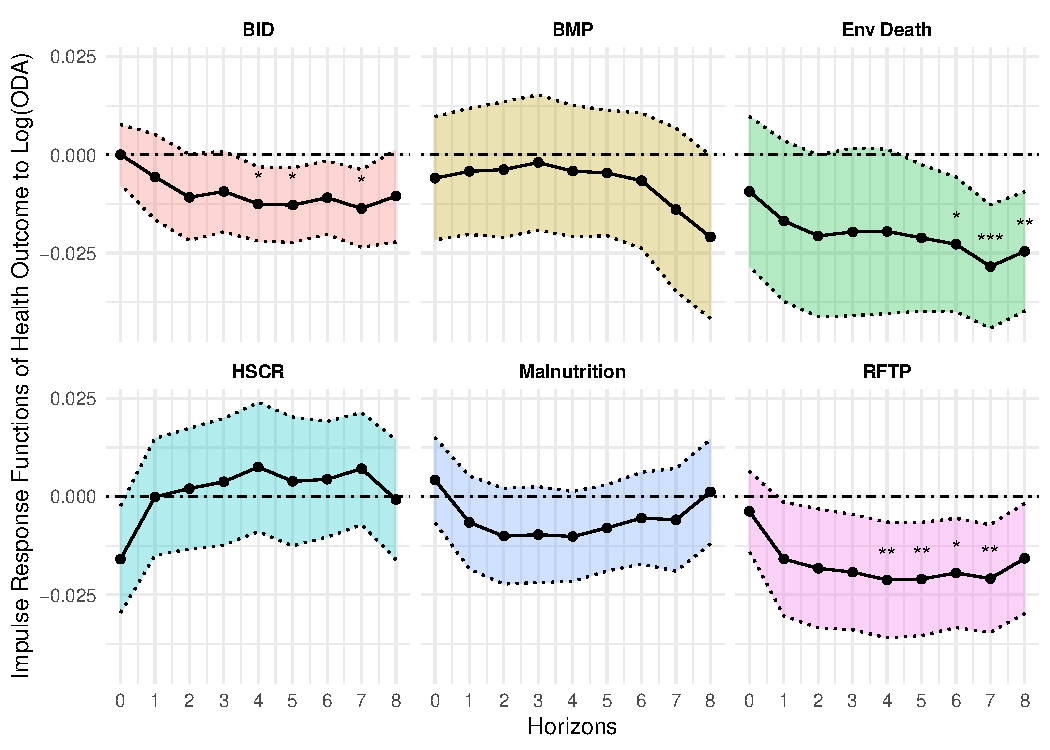
\includegraphics[width = 0.9\textwidth]{Results_outputs/Models/Local_Projt.pdf}
    \caption*{\footnotesize{Note: Author's computation. $^{*}$p$<$0.1; $^{**}$p$<$0.05; $^{***}$p$<$0.01}}
    \label{fig:Local_projection}
\end{figure}

As shown in Figure \ref{fig:Local_projection}, the local projection result is consistent with previously presented methods, showing the anticipated direction of effect for all health dimensions. Accordingly, contemporaneous ODA has positive impacts on the burden of infection and diseases (BID), environmental death, and reproductive fatalities (RFTP), though some effects are weaker than others. Specifically, ODA exhibits the strongest intermediate and long-term effects on reproductive fatalities, with the effect becoming statistically significant after five years (4th horizons) and lasting until the seventh year. While ODA is weakly significant for environmental death after six years (5th horizons), the significance level increases in the seventh and eighth years. Similarly, the impact of ODA on BID is weakly significant, starting from the fourth year and continuing until the seventh year. Surprisingly, ODA now shows positive impact on health system capacity and responsiveness starting from second horizon, albeit none is significant across the horizons. Also, ODA impact change direction on all health dimensions except mental burden, after the seventh year.    

\subsubsection*{\quad 5.2.2 Regional Heterogeneity of ODA Impact on Health Outcomes}
Similar to research question one, the thesis employs a combination of approaches: a unit fixed effect with time trend and FE-CLPM methods, to assess potential regional variations in the impact of ODA across health dimensions. The hypothesis is that:
 \begin{enumerate}[i]
    \item[ii] \textit{$H_0$: The impact of ODA on health is not significantly different between SSA and non-SSA regions on at least one health dimension.}
\end{enumerate} 
To test the hypothesis, the study employs the interaction of specific region dummy variables and one period lag of ODA to isolate the ODA impact in various regions. All models are estimated with five-period mean aggregated data like other models. The followings are the results:
\subsubsection*{\quad \quad \textit{5.2.2.1 Unit Fixed Model Model with Time Trend for Regional Heterogeneity:}}
\renewcommand{\arraystretch}{0.35} % 
\begin{longtable}{@{\extracolsep{-3pt}}lcccccc} 
\caption{Regional Heterogeneity: Unit FE Model with Time Trend}
\\[-0.9ex]\hline 
\hline \\[-0.9ex] 
 & \multicolumn{6}{c}{\textit{Dependent variables:}} \\ 
\cline{2-7} 
\\[-0.9ex] 
 & Reprod. & Infect. \& & Mental & Malnutr- & Envir.  & Health\\
& Fatality & Diseases & Burden & tion & Death & Capacity  \\
\\[-1.8ex] & (1) & (2) & (3) & (4) & (5) & (6)\\ 
\hline \\[-0.9ex]
log(EAP\_ODA)$_{t-1}$             & $0.013$        & $-0.007$       & $0.001$      & $-0.003$       & $0.001$        & $-0.001$      \\
                          & $(0.010)$      & $(0.006)$      & $(0.009)$    & $(0.008)$      & $(0.004)$      & $(0.004)$     \\
                          &&&&&&\\
log(SSA\_ODA)$_{t-1}$    & $-0.005$       & $-0.004$       & $-0.020$     & $0.021$        & $0.010$        & $0.006$       \\
                          & $(0.015)$      & $(0.017)$      & $(0.021)$    & $(0.017)$      & $(0.011)$      & $(0.013)$     \\
                          &&&&&&\\
log(MENA\_ODA)$_{t-1}$   & $-0.027^{*}$   & $0.032^{**}$   & $-0.011$     & $0.002$        & $0.019$        & $0.011$       \\
                          & $(0.012)$      & $(0.012)$      & $(0.018)$    & $(0.013)$      & $(0.016)$      & $(0.006)$     \\
                          &&&&&&\\
log(LAC\_ODA)$_{t-1}$    & $-0.004$       & $0.010$        & $-0.010$     & $-0.003$       & $-0.002$       & $-0.008$      \\
                          & $(0.014)$      & $(0.014)$      & $(0.010)$    & $(0.014)$      & $(0.014)$      & $(0.007)$     \\
                          &&&&&&\\
log(SCA\_ODA)$_{t-1}$    & $-0.022$       & $0.026$        & $0.003$      & $0.030$        & $0.000$        & $0.037$       \\
                          & $(0.036)$      & $(0.035)$      & $(0.043)$    & $(0.018)$      & $(0.041)$      & $(0.027)$     \\
                          &&&&&&\\
log(Europe\_ODA)$_{t-1}$ & $-0.032^{**}$  & $-0.009$       & $-0.016$     & $0.002$        & $-0.041^{*}$   & $-0.009$      \\
                          & $(0.011)$      & $(0.012)$      & $(0.013)$    & $(0.009)$      & $(0.017)$      & $(0.007)$     \\
\hline \\[-0.9ex]
Num.Obs. & \num{576} & \num{576} & \num{576} & \num{576} & \num{576} & \num{576}\\
R2 & \num{0.801} & \num{0.651} & \num{0.355} & \num{0.587} & \num{0.559} & \num{0.617}\\
R2 Adj. & \num{0.725} & \num{0.518} & \num{0.108} & \num{0.429} & \num{0.391} & \num{0.471}\\
AIC & \num{-1820.2} & \num{-1615.0} & \num{-1488.1} & \num{-1751.1} & \num{-1725.0} & \num{-1894.8}\\
BIC & \num{-1746.1} & \num{-1540.9} & \num{-1414.0} & \num{-1677.0} & \num{-1650.9} & \num{-1820.7}\\
RMSE & \num{0.05} & \num{0.06} & \num{0.06} & \num{0.05} & \num{0.05} & \num{0.05}\\
\bottomrule
\multicolumn{7}{l}{\scriptsize{$^{***}p<0.001$; $^{**}p<0.05$; $^{*}p<0.1$}}
\label{table:FE_RQ2}
\end{longtable}
According to the unit fixed effect model shown in Table \ref{table:FE_RQ2}, the impact of ODA weakly varies both across health dimensions and regions. While ODA shows the expected direction of effect on all health dimensions for SSA region except for malnutrition and environmental death, none is significant for the region. Notably, while ODA has positive and mildly significant impact at 5\% on reproductive fatality (RFTP) in the Middle East and North Africa (MENA), it increases burden of infection and diseases in the region. Moreover, ODA has weak significance (at 10\%) on environmental death and reproductive fatality (at 5\%) p\_value in Europe respectively. While the coefficient ODA is positive on health system capacity (HSCR) in SSA, MENA, SCA and Europe, it has negative effect on the dimension in EAP and LAC, albeit none is significant. Aside from these notable differences, the impact of ODA is not significantly different across regions on the rest of the health dimensions.


\subsubsection*{\quad \quad \textit{5.2.2.2 FE-CLDM for Regional Heterogeneity:}}
%list(RFTP_Region_DPM, BID_Region_dpm, BMP_Region_dpm, Malnuti_Region_dpm, EnvDeath_Region_dpm, HSCR_Region_dpm)
\renewcommand{\arraystretch}{0.35} % 
\begin{longtable}{@{\extracolsep{-3pt}}lcccccc} 
\caption{Regional Heterogeneity with FE-CLPM (linear-log model with aggregated data)} 
\\[-1ex]\hline 
\hline \\[-0.9ex] 
 & \multicolumn{6}{c}{\textit{Dependent variables:}} \\ 
\cline{2-7} 
\\[-0.9ex] 
 & Reprod. & Infect. \& & Mental & Malnutr- & Envir.  & Health\\
& Fatality & Diseases & Burden & tion & Death & Capacity  \\
\\[-1ex]
& (1) & (2) & (3) & (4) & (5) & (6)\\ 
\hline \\[-0.9ex]
log(EAP\_ODA)$_{t-1}$                   & $0.005$       & $-0.030$      & $-0.001$      & $-0.041$      & $0.004$       & $0.006$       \\
                                & $(0.011)$     & $(0.023)$     & $(0.024)$     & $(0.023)$     & $(0.018)$     & $(0.017)$     \\
                                &&&&&&\\
log(SSA\_ODA)$_{t-1}$                        & $-0.051$      & $-0.035$      & $-0.043$      & $0.096^{*}$   & $-0.030$      & $0.031$       \\
                                & $(0.030)$     & $(0.045)$     & $(0.053)$     & $(0.043)$     & $(0.040)$     & $(0.041)$     \\
                                &&&&&&\\
log(MENA\_ODA)$_{t-1}$                       & $-0.011$      & $0.061$       & $0.023$       & $0.037$       & $0.011$       & $-0.020$      \\
                                & $(0.020)$     & $(0.031)$     & $(0.039)$     & $(0.032)$     & $(0.036)$     & $(0.029)$     \\
                                &&&&&&\\
log(LAC\_ODA)$_{t-1}$                        & $0.192^{**}$  & $-0.217^{**}$ & $-0.422^{*}$  & $-0.213^{**}$ & $0.264^{**}$  & $-0.284^{**}$ \\
                                & $(0.067)$     & $(0.083)$     & $(0.188)$     & $(0.072)$     & $(0.086)$     & $(0.087)$     \\
                                &&&&&&\\
log(SCA\_ODA)$_{t-1}$                        & $-0.056$      & $-0.088$      & $-0.068$      & $0.239^{***}$ & $-0.008$      & $-0.102$      \\
                                & $(0.039)$     & $(0.068)$     & $(0.080)$     & $(0.067)$     & $(0.050)$     & $(0.064)$     \\
                                &&&&&&\\
log(Europe\_ODA)$_{t-1}$                     & $-0.037$      & $0.031$       & $-0.008$      & $0.058$       & $-0.068^{*}$  & $-0.005$      \\
                                & $(0.021)$     & $(0.029)$     & $(0.035)$     & $(0.032)$     & $(0.030)$     & $(0.029)$     \\
                                &&&&&&\\
%log\_ae                         & $0.037$       & $0.005$       & $-0.073$      & $0.015$       & $-0.032$      & $0.021$       \\
%                                & $(0.055)$     & $(0.059)$     & $(0.078)$     & $(0.049)$     & $(0.041)$     & $(0.055)$     \\
%log\_GDP\_Cap                   & $0.086$       & $-0.022$      & $0.037$       & $-0.052$      & $-0.022$      & $0.234^{***}$ \\
 %                               & $(0.047)$     & $(0.060)$  & $(0.060)$     & $(0.114)$     & $(0.060)$     & $(0.067)$     \\
%FDI                             & $-0.001$      & $-0.001$      & $-0.002$      & $-0.001$      & $-0.001$      & $0.000$       \\
 %                               & $(0.001)$     & $(0.001)$     & $(0.001)$     & $(0.002)$     & $(0.001)$     & $(0.001)$     \\
%log\_CRI\_Score                 & $0.001$       & $0.012$       & $-0.035$      & $-0.013$      & $0.065^{*}$   & $-0.052$      \\
 %                               & $(0.017)$     & $(0.036)$     & $(0.039)$     & $(0.026)$     & $(0.031)$     & $(0.041)$     \\
%log\_Trade                      & $0.013$       & $0.055$       & $0.133^{*}$   & $-0.032$      & $0.058$       & $0.006$       \\
 %                               & $(0.028)$     & $(0.044)$     & $(0.064)$     & $(0.045)$     & $(0.039)$     & $(0.042)$     \\
%log\_hlth\_Per\_Cap             & $0.020$       & $-0.037$      & $0.060$       & $0.016$       & $0.063$       & $0.110^{*}$   \\
%                                & $(0.026)$     & $(0.048)$     & $(0.056)$     & $(0.048)$     & $(0.042)$     & $(0.046)$     \\
%log\_gov                        & $-0.120$      & $0.110$       & $0.063$       & $-0.340^{**}$ & $-0.125$      & $0.156$       \\
 %                               & $(0.069)$     & $(0.083)$     & $(0.109)$     & $(0.110)$     & $(0.093)$     & $(0.093)$     \\
%log\_External\_debt             & $-0.006$      & $-0.022$      & $-0.059^{*}$  & $0.067^{**}$  & $-0.000$      & $-0.008$      \\
 %                               & $(0.016)$     & $(0.018)$     & $(0.024)$     & $(0.021)$     & $(0.018)$     & $(0.019)$     \\
%Autoregressive Parameter   & $0.770^{***}$ &     $0.953^{***}$          &    $0.987^{***}$           &    $0.829^{***}$           &     $0.737^{***}$          &        $0.783^{***}$       \\
 %                               & $(0.043)$     & $(0.093)$       % &   $(0.100)$             &       $(0.096)$        &       $(0.121)$        &    $(0.112)$           \\

Reprod\_Fatality$_{(t - 1)}$ &  $0.770^{***}$  &&&&&\\
&  $(0.043)$ & &&&&\\
&&&&&&\\
Infection\_Diseas$_{(t - 1)}$   &               & $0.953^{***}$ &               &               &               &               \\
                                &               & $(0.093)$     &               &               &               &               \\
&&&&&&\\
Mental\_Burden$_{(t - 1)}$   &               &               & $0.987^{***}$ &               &               &               \\
                                &               &               & $(0.100)$     &               &               &               \\
                                &&&&&&\\
Malnutrition$_{(t - 1)}$   &               &               &               & $0.829^{***}$ &               &               \\
                                &               &               &               & $(0.096)$     &               &               \\
&&&&&&\\
Environ\_Death$_{(t - 1)}$ &               &               &               &               & $0.737^{***}$ &               \\
                                &               &               &               &               & $(0.121)$     &               \\
                                &&&&&&\\
 HealthSys\_Capacity$_{(t - 1)}$     &               &               &               &               &               & $0.783^{***}$ \\
 %                               &               &               &               &               &               & $(0.112)$     \\
\hline \\[-0.9ex]
DF                              & $125.000$     & $125.000$     & $125.000$     & $125.000$     & $125.000$     & $125.000$     \\
Chi-square ($\chi^2$)                           & $280.205$     & $211.046$     & $233.490$     & $259.328$     & $184.373$     & $193.121$     \\
Observation (N)                               & $144.000$     & $144.000$     & $144.000$     & $144.000$     & $144.000$     & $144.000$     \\
RMSEA                           & $0.093$       & $0.069$       & $0.078$       & $0.086$       & $0.057$       & $0.062$       \\
RMSEA 90\% CI Lower                  & $0.078$       & $0.053$       & $0.062$       & $0.071$       & $0.039$       & $0.044$       \\
RMSEA 90\% CI Upper                  & $0.107$       & $0.085$       & $0.093$       & $0.101$       & $0.074$       & $0.078$       \\
p(RMSEA $<$ 0.05)                    & $0.000$       & $0.030$       & $0.003$       & $0.000$       & $0.238$       & $0.134$       \\
SRMR                            & $0.007$       & $0.011$       & $0.011$       & $0.008$       & $0.009$       & $0.009$       \\
\hline
%\multicolumn{7}{l}
%\scriptsize{$^{***}p<0.001$; $^{**}p<0.01$; $^{*}p<0.05$}}
%\end{tabular}
\caption*{\scriptsize{Note: Only the ODA coefficient are presented. ODA estimate represents the EAP region estimate, to avoid binary trap. $^{***}p<0.001$; $^{**}p<0.05$; $^{*}p<0.1$}}
\label{table:DPM_RQ2}
%\end{center}
\end{longtable}


Unlike the unit FE model, the FE-CLPM presented in Figure \ref{table:DPM_RQ2} shows a slightly different result. While the direction of effect is similar to FE model, ODA now has a weak significant effect on environmental death in SSA region. Moreover and surprisingly, the coefficients of ODA across all health dimensions are significant for Latin America and the Caribbean (LAC), albeit positive estimates for environmental death and negative for health system capacity. Due to result inconsistency, it is difficult to conclude that the impact of ODA significantly varies across the regions.  


%is mildly   reveals that the coefficient of the interaction between one-period-lagged ODA and the SSA dummy is statistically significant for infections and diseases. Specifically, a one percentage increase in ODA to the SSA region reduces infections and diseases by 0.075 standard deviations, with significance at the 5\% level, indicating a statistical difference between SSA countries and non-SSA countries. While the coefficients of ODA on other health dimensions show desired directions, except for malnutrition, they are not statistically significant.     

\subsubsection*{\quad 5.2.3 Mediation Path Analysis of Social Protection in ODA's Impact on Health}
\renewcommand{\arraystretch}{0.7} % 
% Table created by stargazer v.5.2.3 by Marek Hlavac, Social Policy Institute. E-mail: marek.hlavac at gmail.com
% Date and time: Tue, Dec 26, 2023 - 08:41:47
\begin{table}[!htbp] \centering 
  \caption{Mediation Analysis of Social Protection in the ODA's Impact on Health Dimensions} 
  \label{tab:MediationModel} 
\begin{tabular}{@{\extracolsep{-3pt}}lcccccc} 
\\[-1.8ex]\hline 
\hline \\[-1.8ex] 
 & \multicolumn{6}{c}{\textbf{Main Predictor: log(ODA)$_{it-4}$}} \\
 & & & & & & \\ 
 & \multicolumn{6}{c}{\textbf{Mediating Variable: Social\_Protection\_Coverage$_{it-3}$}} \\
\cline{2-7} 
\\[-1.8ex] & \multicolumn{6}{c}{ } \\ 
\textbf{Dependent} & Reproductive & Malnutrition  & Infections and & Health & Envir. & Mental\\
\textbf{Variables}: & Fatalities & & Diseases & Capacity & Death & Burden \\
\\[-1.8ex] & (1) & (2) & (3) & (4) & (5) & (6)\\ 
\hline \\[-1.8ex] 
\textbf{Total Effect}: & $-$0.008$^{***}$ & $-$0.015 &$-$0.002 & 0.031 & $-$0.006 & 0.026 \\
 & (0.002)& (0.020)& (0.002)& (0.025) & (0.015)& (0.016)\\
 & & & & & & \\ 
 \textbf{Direct Effect}: & $-$0.008$^{***}$ & $-$0.015 & $-$0.002 & 0.031 & $-$0.006 & 0.026\\
 & (0.002) & (0.020) & (0.002) & (0.025) & (0.015)&  (0.016)\\
 & & & & & & \\  
 \textbf{Indirect Effect}: & $-$0.000 & 0.000 & $-$0.000 & $-$0.000 & 0.000 & $-$0.000\\
 \textbf{Lower CI}: & $-$0.00010 &$-$0.00253 &  $-$0.00005 & $-$0.00245  &  $-$0.00217 & $-$0.00060\\ 
\textbf{Upper CI}: & 0.00006 & 0.00258 & 0.00004 & 0.00218 & 0.00249 & 0.000347 \\
 & & & & & & \\ 
\hline \\[-1.8ex] 
Level of & & & & & & \\
Confidence: & 95\% & 95\% & 95\% & 95\% & 95\% & 95\%\\
Bootstrap &&&&&& \\
Replicates: & 5000 & 5000 & 5000 & 5000 & 5000 & 5000\\
\bottomrule
\hline \\[-1.8ex] 
\textit{Note:}  & \multicolumn{6}{r}{$^{*}$p$<$0.1; $^{**}$p$<$0.05; $^{***}$p$<$0.01} \\ 
\end{tabular} 
\end{table} 



This section presents the result, in Table \ref{tab:MediationModel}, on the mediating role of social protection in the impact of ODA on various health dimensions.
The hypothesis is that:
 \begin{enumerate}[i]
    \item[iii] \textit{$H_0$: The indirect effect of social protection in the impact of ODA on health is not significant on at least one health dimension.}
\end{enumerate} 
For modelling convenience and in line with the causal order: \(ODA_{it-4} \rightarrow SP_{it-3} \rightarrow HO_{it}\) (see Chapter Three, Methodology, for details), year-wave data is employed in the analysis. All relevant variables were demeaned within to reflect the unit FE method, and respective lag and log transformations of relevant variables were performed before modeling. Additionally, a time trend variable was included like other models and the standard errors are corrected using robust error and the bootstrap procedure with 5000 replications across all health dimensions.

The mediation result, in Table \ref{tab:MediationModel}, shows that ODA has a highly significant and positive impact on reproductive fatalities (RFTP), with an average reduction of 0.008 standard deviations in response to a 1\% change in ODA. While ODA exhibits the desired direction of coefficients for other health dimensions, except mental health, they are statistically insignificant. Since the direct effect of all ODA on health remains the same as the total effect, and all confidence intervals of the indirect effect include zero, the result does not provide sufficient evidence that social protection has a significant mediating role in the effect of ODA on all health dimensions. It is important to note that the causal assumption used to derive the indirect effect assumes that treatment (ODA allocation) precedes the mediator (Social Protection), and the mediator, in turn, precedes the outcome (health). Any deviation from these assumptions, such as variations in lag periods, the direction of the relationship, or high missingness of social protection data, could imply potential underestimation or overestimation of the indirect effect. Therefore, this analysis serves as a simple policy guide for the optimal allocation of ODA to enhance health, recognizing its limitations.

\subsection*{5.3 Robustness Checks}
\addcontentsline{toc}{subsection}{5.3 Robustness Checks}
To assess the robustness of the findings presented above, the thesis estimated three models with two approaches. Unit FE with time trend as control and FE-CLDM are estimated for the overaching research question, while only the unit FE is employed for regional heterogeneity. Moreover, the main predictor is now social infrastructure ODA, as opposed to total ODA in the main models. All robustness models employ a similar set of covariates as the main models. Similar to the main models, these robustness models were implemented with aggregated data, and the results are presented in Table \ref{table:DPM_Robst_RQ1}, \ref{table:UnitFE_Robst_Region_RQ2}, and \ref{table:UnitFE_Robst_Region_RQ2}.
\subsubsection*{\quad 5.3.1 Robustness Checks: Impact of Social Infrastructure ODA on Health Outcomes}
\addcontentsline{toc}{subsubsection}{5.3.1 Impact of Social Infrastructure ODA on Health Outcomes}

%\subsection*{Appendix C.2: \quad Roburstness Models}
%\addcontentsline{toc}{subsection}{Appendix C.2: \quad Roburstness Models}
\renewcommand{\arraystretch}{0.35} % 
\begin{longtable}{@{\extracolsep{-3pt}}lcccccc} 
\caption{Robustness Unit FE Model with Social Infrastructure ODA} 
\\[-0.9ex]\hline 
\hline \\[-0.9ex] 
 & \multicolumn{6}{c}{\textit{Dependent variables:}} \\ 
\cline{2-7} 
\\[-0.9ex] 
 & Reprod. & Infect. \& & Mental & Malnutr- & Envir.  & Health\\
& Fatality & Diseases & Burden & tion & Death & Capacity  \\
\\[-1.8ex] & (1) & (2) & (3) & (4) & (5) & (6)\\ 
\hline \\[-0.9ex]
log(SocInfr\_ODA)$_{t-1}$ & $-0.008$       & $-0.027^{**}$  & $0.000$       & $0.015$        & $-0.025$       & $-0.023$      \\
                     & $(0.011)$      & $(0.010)$      & $(0.014)$     & $(0.014)$      & $(0.013)$      & $(0.013)$     \\
                     &&&&&&\\
Elect\_Access                   & $-0.007^{***}$ & $-0.005^{**}$  & $-0.003$      & $-0.003$       & $-0.001$       & $0.005^{***}$ \\
                     & $(0.002)$      & $(0.002)$      & $(0.002)$     & $(0.002)$      & $(0.001)$      & $(0.001)$     \\
                     &&&&&&\\
log(GDP\_PerCap)        & $-0.056$       & $-0.115^{*}$   & $0.032$       & $-0.494^{***}$ & $-0.227^{***}$ & $0.340^{***}$ \\
                     & $(0.083)$      & $(0.053)$      & $(0.075)$     & $(0.108)$      & $(0.066)$      & $(0.057)$     \\
                     &&&&&&\\
Climate\_Risk\_Index           & $0.001$        & $0.000$        & $0.001$       & $0.000$        & $0.001$        & $-0.001^{**}$ \\
                     & $(0.000)$      & $(0.000)$      & $(0.001)$     & $(0.001)$      & $(0.000)$      & $(0.000)$     \\
                     &&&&&&\\
log(Remittance)      & $-0.003$       & $0.002$        & $-0.002$      & $-0.005$       & $-0.004$       & $0.007$       \\
                     & $(0.003)$      & $(0.002)$      & $(0.003)$     & $(0.006)$      & $(0.003)$      & $(0.004)$     \\
                     &&&&&&\\
log(Population)             & $-1.053^{***}$ & $-0.859^{***}$ & $-0.093$      & $-0.645^{*}$   & $-0.065$       & $-0.209$      \\
                     & $(0.311)$      & $(0.223)$      & $(0.524)$     & $(0.295)$      & $(0.407)$      & $(0.194)$     \\
                     &&&&&&\\
log(Pop\_Density)       & $0.313$        & $0.434^{*}$    & $0.189$       & $-0.088$       & $-0.133$       & $0.454^{**}$  \\
                     & $(0.229)$      & $(0.207)$      & $(0.508)$     & $(0.231)$      & $(0.358)$      & $(0.148)$     \\
                     &&&&&&\\
log(Hlth\_Spnd\_PerCap)  & $0.044$        & $0.038$        & $0.106^{*}$   & $-0.075$       & $0.086$        & $0.083^{*}$   \\
                     & $(0.048)$      & $(0.044)$      & $(0.047)$     & $(0.070)$      & $(0.053)$      & $(0.037)$     \\
                     &&&&&&\\
Governance\_Index                  & $-0.044$       & $-0.017$       & $-0.025$      & $-0.166^{***}$ & $-0.063$       & $0.076$       \\
                     & $(0.046)$      & $(0.043)$      & $(0.053)$     & $(0.049)$      & $(0.049)$      & $(0.048)$     \\
                     &&&&&&\\
log(External\_Debt)  & $0.025$        & $0.006$        & $0.006$       & $0.033$        & $-0.023$       & $-0.033^{*}$  \\
                     & $(0.018)$      & $(0.015)$      & $(0.015)$     & $(0.018)$      & $(0.018)$      & $(0.016)$     \\
                     &&&&&&\\
Time\_Trend            & $-0.046^{***}$ & $-0.023^{**}$  & $-0.054^{**}$ & $0.008$        & $-0.063^{***}$ & $0.018$       \\
                     & $(0.011)$      & $(0.009)$      & $(0.017)$     & $(0.013)$      & $(0.016)$      & $(0.011)$     \\
\hline[-0.9ex]
Num.Obs. & \num{576} & \num{576} & \num{576} & \num{576} & \num{576} & \num{576}\\
R2 & \num{0.765} & \num{0.573} & \num{0.251} & \num{0.622} & \num{0.562} & \num{0.583}\\
R2 Adj. & \num{0.678} & \num{0.416} & \num{-0.024} & \num{0.484} & \num{0.401} & \num{0.430}\\
AIC & \num{-1154.3} & \num{-1248.9} & \num{-866.7} & \num{-1007.1} & \num{-1003.5} & \num{-1026.4}\\
BIC & \num{-1102.0} & \num{-1196.6} & \num{-814.4} & \num{-954.8} & \num{-951.2} & \num{-974.1}\\
RMSE & \num{0.09} & \num{0.08} & \num{0.11} & \num{0.10} & \num{0.10} & \num{0.10}\\
\bottomrule
\multicolumn{7}{l}{\scriptsize{$^{***}p<0.001$; $^{**}p<0.05$; $^{*}p<0.1$}}
\label{table:UnitFE_Robst_RQ1}
\end{longtable}

Accordingly, the unit FE model in Table \ref{table:UnitFE_Robst_Region_RQ2}, shows that social infrastructure ODA has positive impact across various health dimensions except malnutrition and health system capacity, albeit insignificant. Moreover, unlike the total ODA, the coefficient of social infrastructure ODA has a positive and mildly significant impact on burden of infection and diseases (BID) with the coefficient value of - 0.027 standard deviations. 
\renewcommand{\arraystretch}{0.35} % 
\begin{longtable}{@{\extracolsep{-3pt}}lcccccc} 
\caption{Robustness FE-CLPM Model with Social Infrastructure ODA} 
\\[-1.8ex]\hline 
\hline \\[-0.9ex] 
 & \multicolumn{6}{c}{\textit{Dependent variables:}} \\ 
\cline{2-7} 
\\[-0.9ex] 
 & Reprod. & Infect. \& & Mental & Malnutr- & Envir.  & Health\\
& Fatality & Diseases & Burden & tion & Death & Capacity  \\
\\[-1.8ex] & (1) & (2) & (3) & (4) & (5) & (6)\\ 
\hline \\[-0.9ex]
log(SocInfr\_ODA)$_{t-1}$            & $-0.065^{***}$ & $-0.077^{***}$ & $-0.137$      & $-0.096^{***}$ & $-0.094^{***}$ & $-0.130^{***}$ \\
                                & $(0.013)$      & $(0.016)$      & $(0.073)$     & $(0.024)$      & $(0.018)$      & $(0.026)$      \\
                                &&&&&&\\
Elect\_Access                              & $0.000$        & $-0.001$       & $-0.001$      & $0.001$        & $0.001$        & $0.003^{*}$    \\
                                & $(0.001)$      & $(0.001)$      & $(0.002)$     & $(0.001)$      & $(0.001)$      & $(0.001)$      \\
                                &&&&&&\\
log(GDP\_PerCap)p                   & $0.053$        & $-0.014$       & $0.073$       & $-0.034$       & $0.010$        & $0.188^{**}$   \\
                                & $(0.037)$      & $(0.069)$      & $(0.070)$     & $(0.096)$      & $(0.052)$      & $(0.069)$      \\
                                &&&&&&\\
log(Remittance)                 & $0.001$        & $0.003$        & $0.008$       & $-0.004$       & $0.003$        & $0.005$        \\
                                & $(0.002)$      & $(0.003)$      & $(0.004)$     & $(0.002)$      & $(0.002)$      & $(0.003)$      \\
                                &&&&&&\\
Climate\_Risk\_Index                      & $-0.000$       & $-0.000$       & $-0.001$      & $-0.001$       & $0.001$        & $-0.001$       \\
                                & $(0.000)$      & $(0.000)$      & $(0.001)$     & $(0.000)$      & $(0.000)$      & $(0.001)$      \\
                                &&&&&&\\
log(Hlth\_Spnd\_PerCap)             & $0.014$        & $-0.050$       & $0.008$       & $0.026$        & $0.099^{*}$    & $0.125^{**}$   \\
                                & $(0.022)$      & $(0.044)$      & $(0.057)$     & $(0.058)$      & $(0.042)$      & $(0.044)$      \\
                                &&&&&&\\
 Governance\_Index                            & $-0.036$       & $0.013$        & $0.027$       & $-0.064$       & $-0.032$       & $0.029$        \\
                                & $(0.028)$      & $(0.036)$      & $(0.069)$     & $(0.042)$      & $(0.043)$      & $(0.041)$      \\
                                &&&&&&\\
log(External\_Debt)             & $0.011$        & $-0.009$       & $-0.056^{**}$ & $0.048^{*}$    & $0.011$        & $-0.003$       \\
                                & $(0.016)$      & $(0.016)$      & $(0.021)$     & $(0.020)$      & $(0.017)$      & $(0.016)$      \\
                                &&&&&&\\
Reprod\_Fatality$_{(t - 1)}$    & $0.760^{***}$  &                &               &                &                &                \\
                                & $(0.036)$      &                &               &                &                &                \\
                                &&&&&&\\
Infection\_Diseas$_{(t - 1)}$   &                & $1.082^{***}$  &               &                &                &                \\
                                &                & $(0.062)$      &               &                &                &                \\
                                &&&&&&\\
Mental\_Burden$_{(t - 1)}$   &                &                & $1.220^{***}$ &                &                &                \\
                                &                &                & $(0.075)$     &                &                &                \\
                                &&&&&&\\
Malnutrition$_{(t - 1)}$   &                &                &               & $0.814^{***}$  &                &                \\
                                &                &                &               & $(0.087)$      &                &                \\
                                &&&&&&\\
Environ\_Death$_{(t - 1)}$  &                &                &               &                & $0.812^{***}$  &                \\
                                &                &                &               &                & $(0.089)$      &                \\
                                &&&&&&\\
HealthSys\_Capacity$_{(t - 1)}$     &                &                &               &                &                & $0.882^{***}$  \\
                                &                &                &               &                &                & $(0.092)$      \\
                                
\hline \\[-0.9ex]
DF                              & $89.000$       & $89.000$       & $89.000$      & $89.000$       & $89.000$       & $89.000$       \\
Chi-square ($\chi^2$)                           & $264.295$      & $212.761$      & $238.637$     & $280.669$      & $150.289$      & $161.800$      \\
Observation (N)                               & $144.000$      & $144.000$      & $144.000$     & $144.000$      & $144.000$      & $144.000$      \\
RMSEA                           & $0.117$        & $0.098$        & $0.108$       & $0.122$        & $0.069$        & $0.075$        \\
RMSEA 90\% CI Lower                  & $0.101$        & $0.081$        & $0.092$       & $0.106$        & $0.049$        & $0.057$        \\
RMSEA 90\% CI Upper                  & $0.133$        & $0.115$        & $0.125$       & $0.139$        & $0.088$        & $0.094$        \\
rmsea.pvalue                    & $0.000$        & $0.000$        & $0.000$       & $0.000$        & $0.054$        & $0.015$        \\
srmr                            & $0.009$        & $0.018$        & $0.020$       & $0.013$        & $0.010$        & $0.009$        \\
\hline
\multicolumn{7}{l}{\scriptsize{$^{***}p<0.001$; $^{**}p<0.05$; $^{*}p<0.1$}}
\label{table:DPM_Robst_RQ1}
\end{longtable}


Similar to the FE-CLPM in the main model, the robustness FE-CLPM model  in Table \ref{table:DPM_Robst_RQ1} shows strong positive and significant impact of social infrastructure ODA for all health dimensions, except the burden of mental problem (BMP) and health system capacity. While the result is consistent with the main models, malnutrition are now strongly significant. Surprisingly, the coefficient of social infrastructure ODA is highly significant and negative for health system capacity, indicating that both social infrastructure and total ODA has exert negative impact on countries health system capacity. Till this end, there is evidence that total and social infrastructure ODA have significant positive impact on reproductive fatality (RFTP), burden of infection and diseases (BID), malnutrition and environmental death. 

\subsubsection*{\quad 5.3.2 Robustness Checks: Regional Variation of Social Infrastructure ODA's Impact}
\addcontentsline{toc}{subsubsection}{5.3.2 Regional Variation of Social Infrastructure ODA's Impact}

Unlike the main regional model, the social infrastructure ODA, as shown the unit FE model in Table \ref{table:UnitFE_Robst_Region_RQ2}, has no significant variation among the regions compared. Specifically, while social infrastructure ODA shows the expected impact on all health dimensions for SSA, except burden of mental problem, none is significant. Similar pattern of result of observed across other regions. Notably,social infrastructure ODA has most negative impact on health system capacity in East Asia and Pacific (EAP) and  Middle East and North Africa (MENA) region, though none is significant.  
\renewcommand{\arraystretch}{0.35} % 
 \begin{longtable}{@{\extracolsep{-3pt}}lcccccc} 
\caption{Robustness Regional Variation with Unit FE for Social Infrastructure ODA} 
\\[-0.9ex]\hline 
\hline \\[-0.9ex] 
 & \multicolumn{6}{c}{\textit{Dependent variables:}} \\ 
\cline{2-7} 
\\[-0.9ex] 
 & Reprod. & Infect. \& & Mental & Malnutr- & Envir.  & Health\\
& Fatality & Diseases & Burden & tion & Death & Capacity  \\
\\[-0.9ex] & (1) & (2) & (3) & (4) & (5) & (6)\\ 
\hline \\[-0.9ex]
log(EAP\_SocInfr\_ODA)$_{t-1}$  & $0.022$        & $-0.002$       & $0.010$       & $-0.003$       & $0.003$        & $-0.014$      \\
                      & $(0.028)$      & $(0.016)$      & $(0.016)$     & $(0.020)$      & $(0.015)$      & $(0.016)$     \\
                      &&&&&&\\
log(SSA\_SocInfr\_ODA)$_{t-1}$      & $-0.017$       & $-0.008$       & $-0.020$      & $0.007$        & $-0.016$       & $0.010$       \\
                      & $(0.031)$      & $(0.024)$      & $(0.022)$     & $(0.026)$      & $(0.016)$      & $(0.021)$     \\
                      &&&&&&\\
log(MENA\_SocInfr\_ODA)$_{t-1}$     & $-0.017$       & $0.002$        & $0.047$       & $0.045$        & $-0.028$       & $-0.004$      \\
                      & $(0.030)$      & $(0.024)$      & $(0.035)$     & $(0.027)$      & $(0.029)$      & $(0.018)$     \\
                      &&&&&&\\
log(LAC\_SocInfr\_ODA)$_{t-1}$      & $-0.034$       & $-0.030$       & $-0.014$      & $0.014$        & $-0.005$       & $0.011$       \\
                      & $(0.032)$      & $(0.018)$      & $(0.018)$     & $(0.023)$      & $(0.021)$      & $(0.018)$     \\
                      &&&&&&\\
log(SCA\_SocInfr\_ODA)$_{t-1}$    & $0.030$        & $0.037$        & $0.006$       & $0.038$        & $0.025$        & $0.038$       \\
                      & $(0.045)$      & $(0.028)$      & $(0.044)$     & $(0.026)$      & $(0.029)$      & $(0.023)$     \\
                      &&&&&&\\
log(Europe\_SocInfr\_ODA)$_{t-1}$ & $-0.054$       & $0.028$        & $-0.039$      & $-0.023$       & $-0.025$       & $0.031$       \\
                      & $(0.037)$      & $(0.054)$      & $(0.060)$     & $(0.031)$      & $(0.071)$      & $(0.019)$     \\
                      &&&&&&\\
Elect\_Access                    & $-0.002^{**}$  & $-0.002^{*}$   & $-0.002$      & $-0.000$       & $0.000$        & $0.003^{***}$ \\
                      & $(0.001)$      & $(0.001)$      & $(0.001)$     & $(0.001)$      & $(0.001)$      & $(0.001)$     \\
                      &&&&&&\\
log(GDP\_PerCap)         & $-0.088$       & $-0.149^{***}$ & $-0.018$      & $-0.284^{***}$ & $-0.102^{**}$  & $0.147^{***}$ \\
                      & $(0.047)$      & $(0.033)$      & $(0.044)$     & $(0.049)$      & $(0.034)$      & $(0.032)$     \\
                      &&&&&&\\
Climate\_Risk\_Index            & $0.000$        & $0.000$        & $0.000$       & $0.000$        & $0.000$        & $-0.001^{*}$  \\
                      & $(0.000)$      & $(0.000)$      & $(0.000)$     & $(0.000)$      & $(0.000)$      & $(0.000)$     \\
                      &&&&&&\\
log(Remittance)       & $-0.001$       & $0.002$        & $-0.002$      & $-0.002$       & $-0.002$       & $0.003$       \\
                      & $(0.001)$      & $(0.002)$      & $(0.002)$     & $(0.003)$      & $(0.002)$      & $(0.002)$     \\
                      &&&&&&\\
log(Population)              & $-0.612$       & $-0.569^{***}$ & $-0.292$      & $-0.127$       & $-0.118$       & $0.149$       \\
                      & $(0.413)$      & $(0.155)$      & $(0.255)$     & $(0.171)$      & $(0.328)$      & $(0.103)$     \\
                      &&&&&&\\
log(Pop\_Density)        & $0.542$        & $0.226$        & $0.140$       & $-0.119$       & $0.135$        & $0.086$       \\
                      & $(0.408)$      & $(0.118)$      & $(0.243)$     & $(0.142)$      & $(0.310)$      & $(0.070)$     \\
                      &&&&&&\\
log(Hlth\_Spnd\_PerCap)   & $-0.001$       & $-0.016$       & $0.073^{*}$   & $-0.063$       & $0.003$        & $0.019$       \\
                      & $(0.025)$      & $(0.031)$      & $(0.035)$     & $(0.040)$      & $(0.027)$      & $(0.019)$     \\
                      &&&&&&\\
Governance\_Index                   & $-0.051$       & $-0.063^{*}$   & $-0.013$      & $-0.077^{**}$  & $-0.042$       & $0.037$       \\
                      & $(0.030)$      & $(0.027)$      & $(0.031)$     & $(0.025)$      & $(0.026)$      & $(0.023)$     \\
                      &&&&&&\\
log(External\_Debt)   & $-0.006$       & $0.013$        & $0.007$       & $0.006$        & $-0.010$       & $-0.019^{*}$  \\
                      & $(0.008)$      & $(0.011)$      & $(0.010)$     & $(0.011)$      & $(0.010)$      & $(0.008)$     \\
                      &&&&&&\\
Time\_Trend             & $-0.065^{***}$ & $-0.026^{***}$ & $-0.023^{**}$ & $-0.003$       & $-0.043^{***}$ & $0.001$       \\
                      & $(0.007)$      & $(0.008)$      & $(0.008)$     & $(0.007)$      & $(0.010)$      & $(0.004)$     \\
\hline \\[-0.9ex]
Num.Obs. & \num{576} & \num{576} & \num{576} & \num{576} & \num{576} & \num{576}\\
R2 & \num{0.800} & \num{0.649} & \num{0.359} & \num{0.595} & \num{0.523} & \num{0.612}\\
R2 Adj. & \num{0.724} & \num{0.515} & \num{0.114} & \num{0.440} & \num{0.341} & \num{0.464}\\
AIC & \num{-1816.7} & \num{-1611.7} & \num{-1492.0} & \num{-1762.1} & \num{-1679.7} & \num{-1887.3}\\
BIC & \num{-1742.6} & \num{-1537.7} & \num{-1417.9} & \num{-1688.0} & \num{-1605.6} & \num{-1813.2}\\
RMSE & \num{0.05} & \num{0.06} & \num{0.06} & \num{0.05} & \num{0.05} & \num{0.05}\\
\bottomrule
\multicolumn{7}{l}{\scriptsize{$^{***}p<0.001$; $^{**}p<0.05$; $^{*}p<0.1$}}
\label{table:UnitFE_Robst_Region_RQ2}
\end{longtable}


%log(SocInfr\_ODA)$_{t-1}$ Elect\_Access log(GDP\_PerCap) Climate\_Risk\_Index log(Remittance) log(Population) log(Pop\_Density) log(Hlth\_Spnd\_PerCap) Governance\_Index log(External\_Debt) Time\_Trend  Reprod\_Fatality$_{(t - 1)}$  Infection\_Diseas$_{(t - 1)}$ Mental\_Burden$_{(t - 1)}$ Malnutrition$_{(t - 1)}$  Environ\_Death$_{(t - 1)}$ HealthSys\_Capacity$_{(t - 1)}$
The FE-CLDM model, on the other hand in Table \ref{table:DPM_Robst_Region_RQ2}, shows more complex result. Accordingly, social infrastructure ODA is found on reproductive fatality, infection and disease and HSCR for EAP, SSA, and MENA regions, all significant at 5\% p\_value. Notably, social infrastructure ODA impact on was also significant on malnutrition for EAP and SSA regions. A possible explanation for these sporadic significance results is that the social infrastructure ODA data employed is commitment, as opposed to disbursement data for total ODA in the main model. Due to inconsistency in results across the regional models and its complexity, the study do not have a conclusive evidence that the impact ODA varies between SSA and non-SSA regions.    

\renewcommand{\arraystretch}{0.35} % 
\begin{longtable}{@{\extracolsep{-3pt}}lccccc} 
\caption{Robustness Regional Variation with FE-CLPM Model for Social Infrastructure ODA} 
\\[-0.9ex]\hline 
\hline \\[-0.9ex] 
 & \multicolumn{5}{c}{\textit{Dependent variables:}} \\ 
\cline{2-6} 
\\[-0.9ex] 
 & Reprod. & Infect. \&  & Malnutr- & Envir.  & Health\\
& Fatality & Diseases & tion & Death & Capacity  \\
\\[-1.8ex] & (1) & (2) & (3) & (4) & (5)\\ 
\hline \\[-0.9ex]
log(EAP\_SocInfr\_ODA)$_{t-1}$            & $-0.111^{**}$ & $-0.087^{*}$  & $-0.150^{*}$  & $-0.049$      & $0.181^{**}$   \\
                                & $(0.036)$     & $(0.044)$     & $(0.074)$     & $(0.035)$     & $(0.066)$      \\
                                &&&&&\\
log(SSA\_SocInfr\_ODA)$_{t-1}$                & $0.128^{**}$  & $-0.054$      & $0.285^{**}$  & $-0.026$      & $-0.276^{**}$  \\
                                & $(0.04 0)$     & $(0.055)$     & $(0.087)$     & $(0.052)$     & $(0.086)$      \\
                                &&&&&\\
log(MENA\_SocInfr\_ODA)$_{t-1}$               & $0.131^{**}$  & $0.072$       & $0.076$       & $-0.003$      & $-0.189^{*}$   \\
                                & $(0.042)$     & $(0.051)$     & $(0.079)$     & $(0.049)$     & $(0.074)$      \\
                                &&&&&\\
log(LAC\_SocInfr\_ODA)$_{t-1}$                & $0.053$       & $0.003$       & $0.092$       & $-0.032$      & $-0.266^{***}$ \\
                                & $(0.041)$     & $(0.050)$     & $(0.077)$     & $(0.042)$     & $(0.074)$      \\
                                &&&&&\\
log(SCA\_SocInfr\_ODA)$_{t-1}$              & $-0.035$      & $0.085$       & $0.193^{*}$   & $0.118$       & $-0.282^{**}$  \\
                                & $(0.058)$     & $(0.066)$     & $(0.086)$     & $(0.072)$     & $(0.107)$      \\
                                &&&&&\\
log(Europe\_SocInfr\_ODA)$_{t-1}$           & $-0.078$      & $-0.140$      & $0.263$       & $-0.355^{*}$  & $-0.499^{**}$  \\
                                & $(0.093)$     & $(0.119)$     & $(0.140)$     & $(0.158)$     & $(0.163)$      \\
                                &&&&&\\
%log(Elect\_Access)                         & $0.063$       & $0.031$       & $0.031$       & $-0.002$      & $0.067$        \\
%                                & $(0.051)$     & $(0.068)$     & $(0.041)$     & $(0.040)$     & $(0.045)$      \\

%log(GDP\_PerCap)                   & $0.065$       & $0.015$       & $-0.045$      & $0.014$       & $0.182^{**}$   \\
  %                              & $(0.046)$     & $(0.072)$     & $(0.124)$     & $(0.054)$     & $(0.062)$      \\

%log(Hlth\_Spnd\_PerCap)             & $0.018$       & $-0.027$      & $0.001$       & $0.095^{*}$   & $0.128^{**}$   \\
 %                               & $(0.022)$     & $(0.045)$     & $(0.057)$     & $(0.042)$     & $(0.044)$      \\
%FDI                             & $-0.001$      & $0.000$       & $-0.001$      & $-0.000$      & $0.001$        \\
 %                               & $(0.001)$     & $(0.001)$     & $(0.002)$     & $(0.001)$     & $(0.001)$      \\
%Climate\_Risk\_Index                 & $-0.019$      & $0.014$       & $-0.017$      & $0.039$       & $-0.069$       \\
 %                               & $(0.016)$     & $(0.038)$     & $(0.025)$     & $(0.026)$     & $(0.040)$      \\
%log(Trade)                      & $0.039$       & $-0.008$      & $-0.012$      & $0.026$       & $-0.036$       \\
 %                               & $(0.031)$     & $(0.040)$     & $(0.052)$     & $(0.032)$     & $(0.047)$      \\
%log(Governance\_Index)                        & $-0.098$      & $0.004$       & $-0.223$      & $-0.106$      & $0.140$        \\
 %                               & $(0.066)$     & $(0.081)$     & $(0.125)$     & $(0.070)$     & $(0.092)$      \\
%log(External\_Debt)             & $-0.007$      & $-0.002$      & $0.039^{*}$   & $0.012$       & $-0.006$       \\
 %                               & $(0.014)$     & $(0.018)$     & $(0.020)$     & $(0.017)$     & $(0.019)$      \\
Reprod\_Fatality$_{(t - 1)}$    & $0.781^{***}$ &               &               &               &                \\
                                & $(0.042)$     &               &               &               &                \\
                                &&&&&\\
Infection\_Diseas$_{(t - 1)}$   &               & $1.018^{***}$ &               &               &                \\
                                &               & $(0.064)$     &               &               &                \\
                                &&&&&\\
Mental\_Burden$_{(t - 1)}$  &               &               & $0.808^{***}$ &               &                \\
                                &               &               & $(0.095)$     &               &                \\
                                &&&&&\\
Malnutrition$_{(t - 1)}$ &               &               &               & $0.749^{***}$ &                \\
                                &               &               &               & $(0.089)$     &                \\
                                &&&&&\\
HealthSys\_Capacity$_{(t - 1)}$    &               &               &               &               & $0.786^{***}$  \\
                                &               &               &               &               & $(0.091)$      \\
\hline \\[-0.9ex]
DF                              & $125.000$     & $125.000$     & $125.000$     & $125.000$     & $125.000$      \\
Chi-square ($\chi^2$)                          & $310.725$     & $266.087$     & $294.130$     & $218.675$     & $185.185$      \\
Observation (N)                               & $144.000$     & $144.000$     & $144.000$     & $144.000$     & $144.000$      \\
RMSEA                           & $0.102$       & $0.089$       & $0.097$       & $0.072$       & $0.058$        \\
RMSEA 90\% CI Lower                  & $0.087$       & $0.074$       & $0.083$       & $0.056$       & $0.039$        \\
RMSEA 90\% CI Upper                  & $0.116$       & $0.103$       & $0.111$       & $0.088$       & $0.075$        \\
p(RMSEA $<$ 0.05)                    & $0.000$       & $0.000$       & $0.000$       & $0.014$       & $0.226$        \\
SRMR                            & $0.006$       & $0.012$       & $0.004$       & $0.006$       & $0.005$        \\
\hline
\multicolumn{6}{l}{\scriptsize{$^{***}p<0.001$; $^{**}p<0.05$; $^{*}p<0.1$}}
\label{table:DPM_Robst_Region_RQ2}
\end{longtable}

      %Environ\_Death$_{(t - 1)}$ 

%the direction of the effect remains consistent with the main fixed effect model using total ODA, Social Infrastructure ODA exhibits significant impacts, particularly demonstrating the strongest effect on infections and diseases, and a weak effect on environmental death, and even an unexpected negative effect on health system capacity. Specifically, Social Infrastructure ODA, on average, reduces infections and diseases by 0.036 standard deviations and is highly significant. Moreover, environmental death is similarly impacted by Social Infrastructure ODA, with coefficients of -0.030, significant at a 5\% p-value. This result aligns with the GMM model presented in Table \ref{table:GMM_table}. While the direction of the effect for reproductive fatalities aligns with expectations, it is statistically insignificant, and health system capacity surprisingly exhibits a negative effect and is weakly significant.
%\renewcommand{\arraystretch}{0.85} % 

% Table created by stargazer v.5.2.3 by Marek Hlavac, Social Policy Institute. E-mail: marek.hlavac at gmail.com
% Date and time: Tue, Dec 26, 2023 - 09:18:33
\begin{table}[!htbp] \centering 
  \caption{Roburstness Check of Regional Variation with Social Infrastructure ODA} 
  \label{Tab:Robust_FE_RegHet} 
\begin{tabular}{@{\extracolsep{-2pt}}lcccccc} 
\\[-1.8ex]\hline 
\hline \\[-1.8ex] 
& \multicolumn{6}{c}{\textit{Dependent Variables:}} \\ 
\cline{2-7} 
\\[-1.8ex] & \multicolumn{6}{c}{ } \\ 
 & Reprod. & Malnutr-  & Infect. \& & Health & Envir. & Mental\\
 & Fatalities & ition & Diseases & Capacity & Death & Burden \\
 
\\[-1.8ex] & (1) & (2) & (3) & (4) & (5) & (6)\\ 
\hline \\[-1.8ex] 
  log(SOC\_INF\_ODA)$_{t-1}$ & $-$0.024$^{*}$ & 0.007 & $-$0.027$^{***}$ & $-$0.027$^{*}$ & $-$0.029$^{*}$ & 0.020 \\ 
  & (0.013) & (0.016) & (0.009) & (0.016) & (0.016) & (0.018) \\ 
  & & & & & & \\ 
 log(SOC\_INF\_ODA)$_{t-1}\times$SSA & 0.015 & 0.002 & $-$0.037 & 0.018 & $-$0.006 & $-$0.034 \\ 
  & (0.050) & (0.048) & (0.039) & (0.031) & (0.031) & (0.041) \\ 
  & & & & & & \\ 
log(Govt\_Hth\_Spnd) & $-$0.065 & $-$0.053 & $-$0.020 & 0.084$^{**}$ & $-$0.027 & 0.093$^{***}$ \\ 
  & (0.053) & (0.040) & (0.034) & (0.033) & (0.032) & (0.034) \\ 
  & & & & & & \\ 
 log(GDP\_per\_cap) & $-$0.162$^{**}$ & $-$0.239$^{***}$ & $-$0.183$^{***}$ & 0.196$^{***}$ & $-$0.308$^{***}$ & $-$0.054 \\ 
  & (0.081) & (0.073) & (0.056) & (0.058) & (0.053) & (0.063) \\ 
  & & & & & & \\ 
 log(Pop\_tot) & 0.024$^{***}$ & 0.034$^{***}$ & $-$0.015$^{*}$ & $-$0.018$^{***}$ & 0.024$^{**}$ & $-$0.021$^{*}$ \\ 
  & (0.008) & (0.009) & (0.008) & (0.007) & (0.010) & (0.012) \\ 
  & & & & & & \\ 
 Electricity\_access & $-$0.012$^{***}$ & $-$0.006$^{***}$ & $-$0.007$^{***}$ & 0.008$^{***}$ & $-$0.004$^{***}$ & $-$0.001 \\ 
  & (0.002) & (0.001) & (0.002) & (0.001) & (0.001) & (0.002) \\ 
  & & & & & & \\ 
 log(External\_debt) & 0.049$^{**}$ & 0.048$^{***}$ & 0.009 & $-$0.053$^{***}$ & $-$0.022 & 0.008 \\ 
  & (0.021) & (0.018) & (0.015) & (0.013) & (0.016) & (0.016) \\ 
  & & & & & & \\ 
 log(Trade) & $-$0.053 & 0.048 & 0.032 & $-$0.034 & 0.023 & 0.003 \\ 
  & (0.067) & (0.063) & (0.041) & (0.044) & (0.045) & (0.046) \\ 
  & & & & & & \\ 
 CRI\_score & 0.001$^{**}$ & 0.0003 & 0.001 & $-$0.001$^{***}$ & 0.001$^{*}$ & 0.001 \\ 
  & (0.001) & (0.001) & (0.0004) & (0.0004) & (0.0004) & (0.001) \\ 
  & & & & & & \\ 
 Governance & $-$0.049 & $-$0.220$^{***}$ & 0.025 & 0.081 & $-$0.044 & $-$0.039 \\ 
  & (0.058) & (0.055) & (0.044) & (0.065) & (0.051) & (0.058) \\ 
  & & & & & & \\ 
 FDI & $-$0.002 & $-$0.003$^{*}$ & $-$0.001 & 0.002$^{*}$ & $-$0.0003 & $-$0.0003 \\ 
  & (0.001) & (0.001) & (0.001) & (0.001) & (0.001) & (0.001) \\ 
  & & & & & & \\ 
 log(Pop\_densty) & $-$0.093$^{**}$ & $-$0.054$^{**}$ & $-$0.102$^{***}$ & $-$0.026 & $-$0.096$^{***}$ & $-$0.015 \\ 
  & (0.041) & (0.027) & (0.034) & (0.029) & (0.025) & (0.042) \\ 
  & & & & & & \\ 
 time\_var & $-$0.057$^{***}$ & $-$0.049$^{***}$ & $-$0.021$^{***}$ & 0.037$^{***}$ & $-$0.050$^{***}$ & $-$0.032$^{**}$ \\ 
  & (0.008) & (0.009) & (0.006) & (0.008) & (0.010) & (0.013) \\ 
  & & & & & & \\ 
 \hline \\[-1.8ex] 
Num.Obs. & \num{720} & \num{720} & \num{720} & \num{720} & \num{720} & \num{720}\\
R2 & \num{0.749} & \num{0.676} & \num{0.656} & \num{0.640} & \num{0.667} & \num{0.187}\\
R2 Adj. & \num{0.680} & \num{0.586} & \num{0.560} & \num{0.540} & \num{0.575} & \num{-0.039}\\
AIC & \num{-967.4} & \num{-971.5} & \num{-1214.1} & \num{-1043.9} & \num{-993.7} & \num{-707.1}\\
BIC & \num{-903.2} & \num{-907.4} & \num{-1150.0} & \num{-979.8} & \num{-929.6} & \num{-643.0}\\
RMSE & \num{0.12} & \num{0.12} & \num{0.10} & \num{0.11} & \num{0.12} & \num{0.15}\\
\bottomrule
\hline \\[-1.8ex] 
\textit{Note:}  & \multicolumn{6}{r}{$^{*}$p$<$0.1; $^{**}$p$<$0.05; $^{***}$p$<$0.01} \\ 
\end{tabular} 
\end{table} 

%In the second set of robustness checks presented in Table \ref{Tab:Robust_FE_RegHet}, using the same model while adjusting for regional heterogeneity, Social Infrastructure ODA's impact is not significant on any health dimensions in SSA countries, unlike the total ODA. However, the significance of Social Infrastructure ODA on certain health dimensions, such as infections and diseases, environmental death, and health system capacity, observed in the first general robustness model above, is evident in non-SSA countries. Specifically, a 1\% increase in social infrastructure ODA, on average, reduces infections and diseases by 0.027 standard deviations, and this effect is highly significant in non-SSA countries. Additionally, other health dimensions, such as reproductive fatalities and environmental death, are similarly impacted by Social Infrastructure ODA with estimates of -0.024 and 0.029 standard deviations, respectively, but both are weakly significant.

\subsection*{5.4 Summary of Findings}
\addcontentsline{toc}{subsection}{5.4 Summary of Findings}
The key findings from the analyses are summarized as follows:

\begin{enumerate}[i]
    \item The impact of Official Development Assistance (ODA) on health is mix and varies based on the type of ODA, econometric model employed, and health dimensions considered. Despite these variations, both total and social infrastructure ODA demonstrate significant positive impacts on certain health dimensions, such as reproductive fatality, infections and diseases, and environmental death health dimensions. These consistent findings are observed across the fixed effect, FE-CLPM, local projection, and robustness models. 
    \item Moreover, the impact ODA on malnutrition is equally positive and significant, but the result is only evident in the FE-CLPM models, which is the main study model. While social infrastructure ODA tends to be more impacting on infection and diseases, compared to total ODA which is more effective on reproductive fatality. Therefore, against the null hypothesis, there is evidence that ODA has significant positive impact on at least one of the health dimensions being considered.
    \item Surprisingly, the study does not find evidence that foreign aid (ODA) has any significant impact on health system capacity (HSCR).

    \item Utilizing year-wave data, the local projection models presented in Figure \ref{fig:Local_projection} reveal that ODA has both intermediate (5 years) and long-term (six years) effects on reproductive fatalities and infections and diseases, with the effect being stronger in the formal than the later. The impact of ODA on environmental death is long-term, with the effect materializing six years after ODA disbursement. 

    \item Regarding the regional heterogeneity of both total and social infrastructure ODA impact, there are variations in the pattern of effect across models. Due to the inconsistent findings across the regional models, there is no evidence that ODA impact is significantly different for SSA and non-SSA regions.  
    
   % In terms of regional variation in effect, the impact of total ODA significantly differs for Sub-Saharan Africa (SSA) countries, especially in the context of infections and diseases. Conversely, social infrastructure ODA demonstrates greater significance for non-SSA countries, particularly across infections and diseases, reproductive fatalities, and environmental death.

    \item The mediation analysis does not provide sufficient evidence to support the notion that social protection plays an indirect role in the impact of ODA on health. Due to the limitations associated with social protection data and causal order assumptions, there exists a potential for underestimation or overestimation. Therefore, these findings are presented as a pragmatic policy guide for optimizing ODA allocation rather than definitive conclusions.
\end{enumerate}


\section*{\centering Chapter Six}
\section*{\centering Discussion of Findings, Conclusions and Recommendations}
%\addcontentsline{toc}{section}{Chapter Six}
\addcontentsline{toc}{section}{Chapter Six: Discussion of Findings, Conclusions and Recommendations}
The chapter presents the discussion of key findings from the analyses and further contextualizes them within the existing studies. Furthermore, it draws major conclusions and relevant policy implications. The chapter ends with study limitations and suggestions for future studies. 
\subsection*{6.1 Discussion of Findings}
\addcontentsline{toc}{subsection}{6.1 Disscusion of Findings}
\subsubsection*{\quad 6.1.1 Impact of ODA on Health outcomes}
\addcontentsline{toc}{subsubsection}{6.1.1 Impact of ODA on Health outcomes}
The overarching objective of this thesis is to evaluate the impact of Official Development Assistance (ODA) on health outcomes in developing countries. According to the findings, the impact of ODA vary based on ODA type, specific health dimensions, and the chosen econometric approach. Despite this variability, the analysis reveals that ODA has notable impact on specific health dimensions. Both the unit fixed effect and Fixed Effect Cross-lag Panel  Models (FE-CLPM), for instance, demonstrate that ODA significantly reduces reproductive fatality (RFTP), burden of Infection and Diseases (BID), and environmental deaths. These findings are further strengthened in the local projection model, where ODA demonstrates both intermediate and long-term significant effects on these three health dimensions. 
While these composite health dimensions are unique to this study, prior research has consistently shown similar findings on specific indicators aggregated within them. Using adult death—embedded in reproductive fatality and environmental, for instance, death—\textcite{yan_mortality_2015} reveals that the Global Health Fund had a significant effect on mortality rates in developing countries. Comparable findings are reported by \textcite{doucouliagos_health_2021} and \textcite{kavanagh_governance_2019} on the significant impact of ODA on child mortality, a component embedded in the RFTP health dimension.

Moreover, a study on the impact of the Mexico City Policy (MCP), aimed at reducing USA ODA on reproductive health, by \textcite{kavakli_us_2022} reported a significant rise in maternal and child mortality, as well as HIV incidence—crucial indicators in the burden of infection and diseases (BID) and RFTP health dimensions. These findings are supported by a range of other studies \parencite{akinola_foreign_2022, muhammad_health_2021, yogo_health_2015}, all of which reveal the positive impact of ODA on respective health indicators aggregated in the thesis's health dimensions. Contrary findings, however, have been reported in numerous other studies \parencite{williamson_foreign_2008, nwude_official_2020, bavinger_relationship_2017, toseef_how_2019}. These findings bear relevance to this study because the specific indicators employed are embodied in the thesis's health dimensions, particularly BID, environmental death, as well as RFTP.

Notably, one reason for disparities among studies could be attributed to the lag period of ODA. Since ODA does not have an immediate effect on health, studies with unlagged ODA are less likely to reveal the desired result due to model misspecification. As shown in the local projection Figure \ref{fig:Local_projection}, the causal response of ODA on health dimensions manifests significantly after four years following allocation. Previous studies, such as those by \textcite{kavanagh_governance_2019}, \textcite{kavakli_us_2022}, \textcite{chung_economic_2022}, and \textcite{akinola_foreign_2022}, employed lagging ODA with a first-order lag, while \textcite{doucouliagos_health_2021} used a five-year lag, consistent with the approach adopted in this thesis and revealed similar findings.

In addition, the FE-CLPM model shows both total and social infrastructure ODA have significant positive impact on malnutrition. It's noteworthy that this effect is distinctive to the FE-CLPM model and is not observed in other models. This findings is novel, given the limited existing research exploring this specific area.
Moreover, the analysis indicates that none of the types of Official Development Assistance (ODA) has the desired impact on Health System Capacity and Responsiveness (HSCR). Surprisingly, all coefficients of ODA on this health dimension were consistently negative across models. While studies examining the influence of ODA on health system capacity in developing countries are limited, a qualitative study by \textcite{cassola_evaluating_2022} suggests that ODA has little or no effect on the health research landscape in developing countries, aligning with the findings of this thesis. This alignment may contribute to the perspectives of aid pessimists, including \textcite{easterly_aid_2004}, who posit that the inefficacy of foreign aid stems from its emphasis on treatment rather than prevention.  Furthermore, none of the models yield noteworthy findings on the impact of ODA on the burden of mental problems (BMP). Comparison with other studies on this health dimension is challenging due to the elusive nature of mental health. Moreover, this pattern of findings and the lack of study could also be a consequence of the lower incidence of mental problems in underdeveloped countries, which are the major recipients of ODA.




\subsubsection*{\quad 6.1.2 Regional Heterogeneity of ODA Impact on Health}
\addcontentsline{toc}{subsubsection}{6.1.2 Regional Heterogeneity of ODA Impact on Health}

The study reveals inconsistent evidence regarding regional variations in the impact of ODA on health outcomes, as both types of total ODA only vary across region for certain health dimensions. Specifically, in the main model, the impact of total ODA on burden of infection and diseases and reproductive fatality are significant in MENA while reproductive fatality and environmental death is significant in Europe. However, none of the coefficient of ODA is significant across all health dimensions for SSA region. Surprisingly, in the robustness FE-CLPM, social infrastructure ODA is found to be weakly significant for Reproductive Fatality and Teen Pregnancy (RFTP), Burden of Infection and Diseases (BID), and malnutrition for East Asia and Pacific (EAP) and Middle East and North Africa (MENA) regions. However, it is mildly significant only on RFTP and malnutrition for the SSA region. 


Additionally, among all the regions, social infrastructure ODA is only positive and mildly significant on health system capacity (HSCR) for EAP region. Due to inconsistency in the result, the study finds no evidence that the impact of ODA significantly vary among the regions. While these findings may be controversial, similar results have been reported. Utilizing only health ODA, \textcite{nwude_official_2020} found no regional variation in the impact of ODA on life expectancy between SSA and non-SSA regions. Although life expectancy is not part of the thesis health dimensions, health ODA is a subsector of social infrastructure ODA used in this thesis. Moreover, across other studies \parencite{gama_health_2015, staicu2017study, shafiullah_foreign_2011} with regional comparing found no significant difference in the impact of ODA on education, income, and inequality—all of which are essential predictors of health outcomes, between SSA and non-SSA regions.


\subsubsection*{\quad 6.1.3  Mediating Role of Social Protection in the Impact of ODA on Health Outcome}
\addcontentsline{toc}{subsubsection}{6.1.3 Mediating Role of Social Protection}

In exploring the impact of ODA on various health dimensions, this thesis assesses the possible mediating role of social protection. Surprisingly, the indirect effect of social protection insignificant, with a confidence interval encompassing zero for all health dimensions. Thus, social protection does not mediate any effect of ODA across all health dimensions. While this form of mediation analysis is novel in the assessment of ODA effectiveness on health, making comparisons with existing studies challenging.

It is crucial to note, however, that these findings do not necessarily imply that ODA does not influence social protection, as indicated by \textcite{nino-zarazua_aids_2023}, or that social protection does not affect health outcomes, as evidenced by studies such as \textcite{sepehri_how_2014, sarkodie_effect_2021, heggebo_disentangling_2020, adato_social_2009}. The limitation encountered in social protection data and the assumed causal order may underestimate the social protection indirect effect, thus influencing the thesis findings. Therefore, the specific finding is intended solely as a preliminary policy guide for the optimal allocation of ODA, rather than a definitive conclusion. Nevertheless, \textcite{yogo_health_2015} identified female education and government spending as mediators of ODA impact on health in their study, adding complexity to the understanding of mediating factors in the relationship between ODA and health.


\subsection*{6.2 Conclusions}
\addcontentsline{toc}{subsection}{6.2 Conclusion}

In light of the findings, the thesis concludes that ODA, particularly in the form of social infrastructure and total net ODA, have positive and significant impact on health outcomes. However, this impact is health dimension-specific, with both total and social infrastructure ODA demonstrating a more pronounced effect on infections and diseases, reproductive fatality, and environmental death. There is no also an evidence ODA may have a positive impact on malnutrition, albeit weak. Notably, there is no evidence that ODA enhances the health system capacity and responsiveness, which is crucial to ensuring sustainable health security in developing countries. Furthermore, the significance of ODA is contingent on the health priorities of the region, as revealed in the thesis analysis. Lastly, the thesis does not have any conclusive evidence regarding social protection as a potential mediator for improving health outcomes. 


While this research contributes valuable insights to the body of evidence on foreign aid effectiveness, the inconclusiveness observed in previous studies on ODA and health outcomes may be attributed to variations in specific health indicators, econometric approaches, and the specific types of ODA employed. It is crucial to recognize that there is no universally superior model, as threats to validity can only be mitigated, not eliminated. Thus, understanding the true causal impact of ODA on health necessitates a comprehensive examination of a multitude of evidence, including insights from previous studies in developing countries.

% it is important to acknowledge certain limitations, including the causal assumption, data quality, and model specifications, that may have influenced the results.
  
 
\subsection*{6.3 Policy Recommendations}
\addcontentsline{toc}{subsection}{6.3 Policy Recommendations}
In light of the study's findings, the thesis proposes the following policy recommendations to optimize the impact of global development efforts:
\begin{enumerate}[i]
    \item \textbf{Prioritizing Critical health infrastructure in global development effort:} Shifting the focus of global development efforts towards investing in critical health infrastructure, including healthcare facilities, medical personnel, and preventive healthcare measures is crucial for sustainable global health security. This emphasizes the need for long-term investments in critical health infrastructures to enhance a developing nation's self-reliance in managing health challenges. This approach aligns with the principles of sustainable development by promoting autonomy and resilience in healthcare systems. 
   
    \item \textbf{ODA Allocation Mechanisms Strengthening :} Preliminary findings indicate that ODA allocation pattern does not depend on countries' health situations or needs. Strengthening the capacity of the Development Assistance Committee (DAC) and adopting a result-based financing approach can enhance the effectiveness of ODA by directing funds where they are most needed and can have the greatest impact. Targeted ODA allocation based on countries' health situations and needs will improve the effectiveness of aid in addressing specific health challenges. This recommendation aims to ensure that ODA is allocated efficiently, addressing specific health challenges in recipient countries.
    
    \item \textbf{Optimal  Utilization of ODA by Recipient Governments:} A holistic and strategic approach by recipient governments is essential to realizing the full potential of foreign aid. Thus, recipient governments should adopt a visionary approach, focusing on policies that enhance healthcare systems, poverty alleviation, education, social protection, and health research. Strategic utilization of ODA by recipient governments will enhance absorptive capacity, ensuring that aid is optimally used for sustainable development.  
    
    \item \textbf{Governance and Accountability:} While the impact of governance on ODA effectiveness is beyond the scope of this study, governance emerges as a crucial factor in all models. Governance deficiencies, such as corruption and ineffectiveness, impede ODA effectiveness. Therefore, there is need to address governance deficiencies by implementing international sanctions for governments mismanaging ODA, including prevention from future access or requests for ODA return. This recommendation aims to curb corruption and ineffectiveness, enhancing accountability and ensuring that aid funds are used transparently for their intended purposes. Good governance practices are crucial for the successful implementation and impact of foreign aid
    
    \item \textbf{Focus on Economic Development, Debt Forgiveness, and Conflict Prevention:} Recognizing the interconnected nature of development challenges, the thesis advocates for a comprehensive approach that prioritizes economic development, debt forgiveness, and conflict prevention alongside ODA allocation. Excessive debt and economic instability in developing countries contribute significantly to poverty and poor health outcomes. Therefore, the international community, alongside specific developing countries, should prioritize initiatives that create an environment conducive to sustainable development. This holistic strategy addresses underlying factors and emphasizes the interconnected nature of development issues, ultimately contributing to the improvement of overall well-being.
\end{enumerate}

%Based on the findings, the thesis concludes that ODA, particularly social infrastructure ODA has a significant effect on health outcomes. However, this impact is health dimension-specific. For instance, both total and social infrastructure ODA has more impact on infections and diseases, reproductive fatality, and as well as environmental death. Also, there is no evidence that ODA enhances health system capacity and responsiveness in developing countries.  It is essential to note, that much of the inconclusiveness of previous studies on ODA and health outcomes could be attributed to variation in specific indicators employed, econometric approach, and specific type of ODA employed. Moreover, while the total ODA tends to be more significant for infection and diseases in the SSA region, social infrastructure ODA is more significant on health in non-SSA regions. Based on this, the thesis concludes that the significance of ODA depends on the health priority of the region, as shown across the thesis analysis. Finally, the thesis does not have any conclusive evidence of social protection as a potential mediator for improving health outcomes. 

%Based on the findings, the thesis offers the following policy recommendations: 
%\begin{itemize}
 %   \item As revealed in the preliminary findings, ODA is barely allocated to where they are needed the most. To ensure adequate ODA effectiveness, more mechanisms are needed on the supply side of ODA to ensure ODA is allocated to areas where they are most needed. Such mechanism may be through to enhance the capacity of the Development Assistance Committee (DAC) of the OECD as well as the result-based financing approach.  
  %  \item Moreover, recipient governments and countries need to be more visionary on how they utilize the received ODA. Since deficit in health investment and entrenched poverty are the major causes of poor health, ODA recipient governments should focus their attention on policies that enhance their healthcare system and also reduce poverty. Such a policy approach is an investment in education, social protection, and health research to build essential absorptive power for ODA effectiveness.  
   % \item Furthermore, even though the impact of governance on ODA effectiveness is beyond the scope of this study, it is evident from all the models that governance is essential to any kind of development, particularly health. Governance deficiency like corruption and ineffectiveness hampers ODA effectiveness. Therefore, there is need for international sanctions for governments that mismanage ODA allocated to their respective countries. Such sanction may include prevention from future access to ODA or request for returning the ODA even if disbursed on grant. This will enhance the sense of accountability among recipient governments. 
   % \item No matter the amount of ODA allocated, lack of economic development and excessive debt in developing countries will continue to enhance poverty and poor health outcomes. Therefore, the international community should focus development efforts on investing in critical infrastructure, debt forgiveness, and preventing war and violence in developing countries. 
%\end{itemize}

\subsection*{6.4 Study Limitations and Suggestions for Future Research}
\addcontentsline{toc}{subsection}{6.4 Study Limitations and Suggestions for Future Research}
While this study investigates not only the effectiveness of ODA but also which health dimensions are most influenced by ODA, there are certain limitations. Future studies may delve into each of the thesis health dimensions to gain a deeper understanding of their respective intricacies. An especially noteworthy area for future exploration is discerning why ODA exhibits a negative impact on health system capacity. If sustainable development is a critical factor in ODA allocation, investigating its effect on health system capacity should be prioritized in subsequent studies.

Despite the absence of evidence on ODA effectiveness on mental problems in this thesis, future research endeavors may further investigate this aspect. Moreover, while the study offers preliminary findings on the ineffectiveness of social protection as a potential channel for ODA's impact on health, the lack of adequate panel data for social protection performance indicators and the potential inconsistency in causal order assumptions might have led to an underestimation of the mediating impact of social protection. Hence, future studies might focus on specific country-level micro-analysis, employing household surveys to comprehend how emergency social protection from received ODA has improved health situations.

Furthermore, although the thesis findings were consistent to some extent, they are sensitive to the econometric approach employed. Therefore, there is a need for further research grounded in the dynamic panel method. One such approach is the Fixed Effect Cross-Lag Panel Model based on Maximum Likelihood Estimation (ML-SEM) by \textcite{allison2017maximum}. While the thesis employed this method, future researchers are encouraged to explore more on this new approach. ML-SEM has been verified in various simulations to yield more consistent and efficient estimates \parencite[see][]{moral2019dynamic, becker2023many, allison2017maximum}.

Finally, the study focused on two forms of ODA—total and social infrastructure ODA. Future studies may consider exploring subsector-specific ODA, such as basic health, to gain more nuanced insights into the specific areas of impact.

%The study strives towards understanding not only ODA effectiveness but also on which health dimension is ODA most effective. Future studies may explore each of thesis health dimensions, for deeper understanding of the respective health dimensions. One notable health dimension for future exploration will be to understand why ODA is negative for health system capacity. If sustainable development is crucial in ODA allocation, scrutinizing its impact on health system capacity should be focused in future studies.  Despite the lack of evidence in the thesis on the impact of ODA on the burden of mental problems, future studies may investigate this further.  Moreover, while the study provides preliminary findings on the ineffectiveness of social protection as a possible channel for ODA impact on health, lack of adequate panel data for social protection performance indicators and the possibility of inconsistent causal order assumption might have underestimated the mediating impact of Social protection. Therefore, future studies may focus on specific country micro-analysis, using household surveys, to understand how the emergency social protection from ODA received has improved health situations. Furthermore, although the thesis findings were consistent to some extent, there sensitivity of findings to econometric approach employed. Therefore, there is a need for further research that is more grounded in the dynamic panel method.
%One of such is the Fixed effect cross lag panel model based on the maximum likelihood estimation of \textcite{allison2017maximum}. Although, the thesis employed this method I encourage the future to try this new approach. ML-SEM has been proven to produce more consistent and efficient estimate \parencite[see][]{leszczensky2022deal, becker2023many, allison2017maximum}. Finally, the study employed two forms of ODA; total and social infrastructure ODA, future studies may focus on subsector-specific ODA such as basic health.  

\end{onehalfspace}  % Use the onehalfspace environment 

%\end{doublespace}

\clearpage
\pagenumbering{roman}

% Include other chapters as needed

\newpage
% Appendices
\appendix
\appendix
\section*{Appendix Section}
\addcontentsline{toc}{section}{APPENDIX}

%\setcounter{figure}{0} % Reset figure counter
%\setcounter{table}{0}  % Reset table counter

\subsection*{Appendix A.1: OECD Classification Methods of ODA}
\addcontentsline{toc}{subsection}{Appendix A.1: OECD Classification Methods of ODA}

\begin{figure}[ht]
\captionsetup{justification=justified,singlelinecheck=false}
\caption{General DAC system of ODA Classification}
    \centering{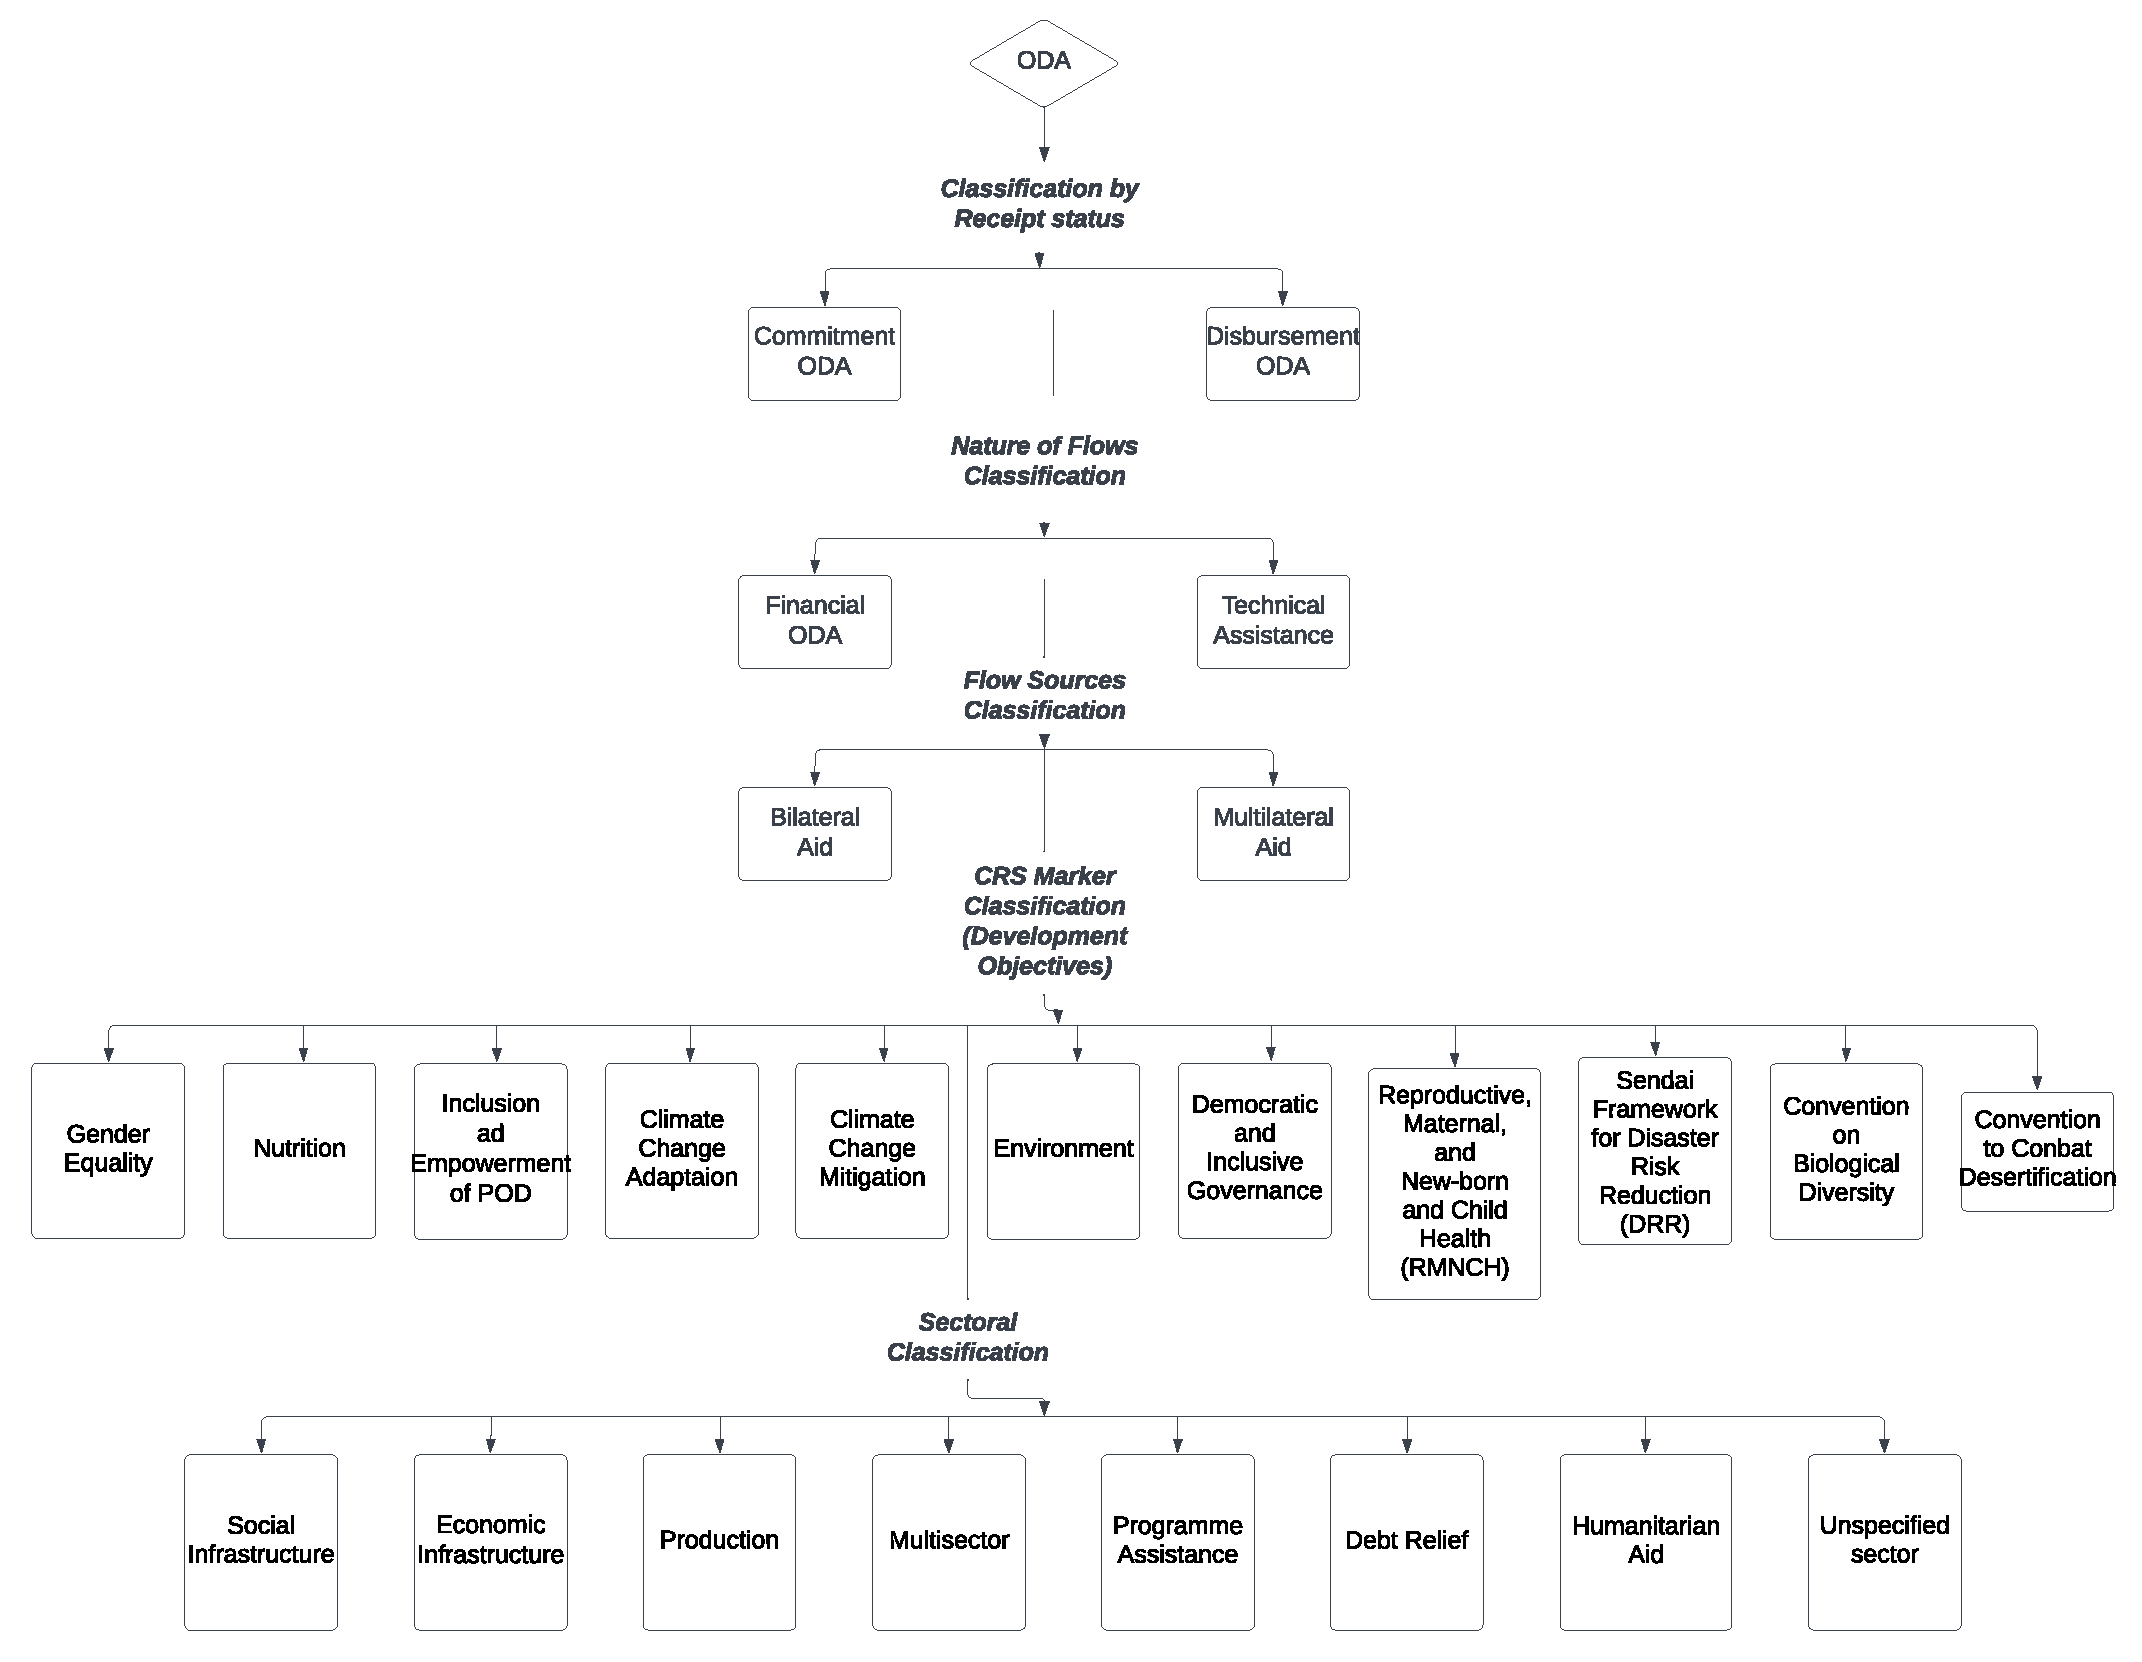
\includegraphics[width = 0.8\textwidth, height = 8cm]{Appendices/ODA classification system/Classifications system of ODA.pdf}}
    \label{fig:General ODA classification}
    \caption*{\footnotesize{Author's illustration, adapted from \textcite{oecd_Data_2023}. Image used to show the different levels of classification used at the OECD for compiling ODA data.}}
\end{figure}

\begin{figure}[H]
\captionsetup{justification=justified,singlelinecheck=false}
\caption{OECD ODA Sectors Classification}
    \centering{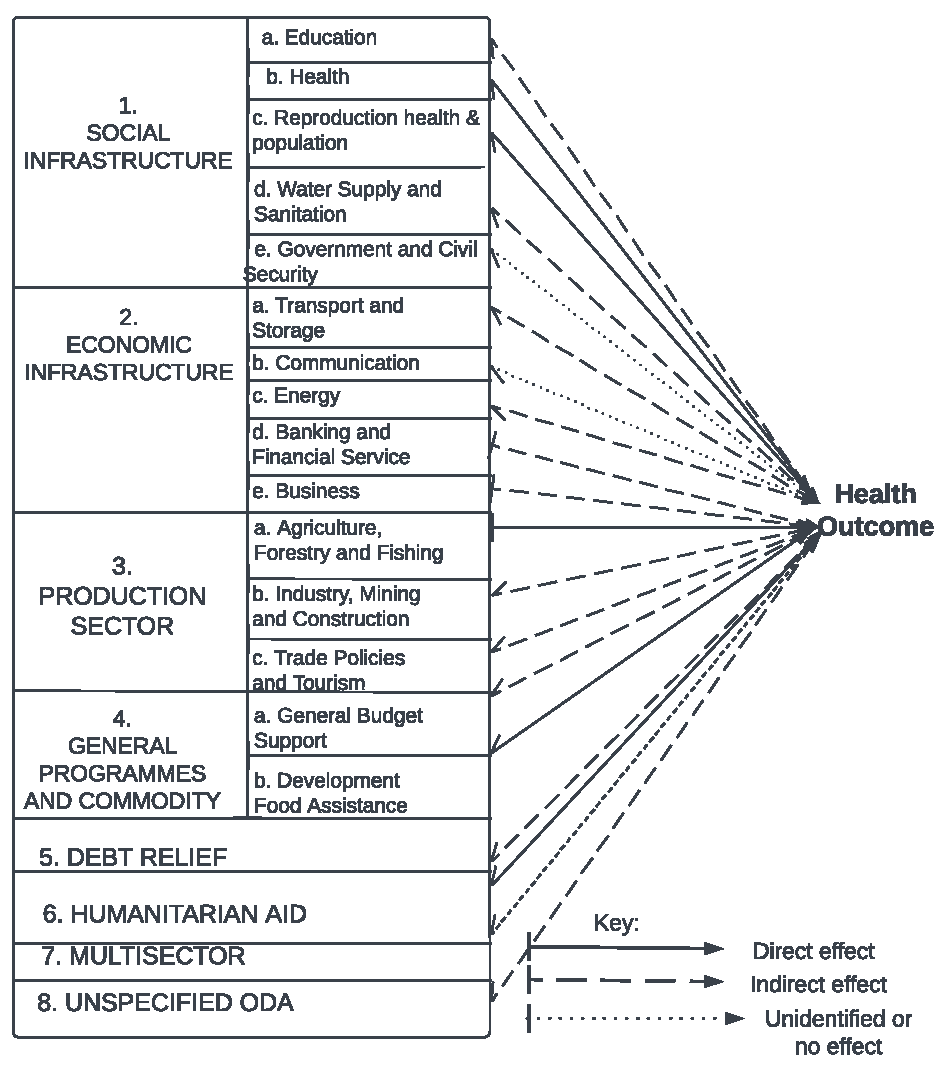
\includegraphics[width = 0.75\textwidth, height  = 9cm]{Appendices/ODA classification system/ODA and Health flows.pdf}}
    \label{fig:Sector ODA classification}
    \caption*{\footnotesize{Author's illustration, adapted from \textcite{oecd_Data_2023}. Image used to justify the use of total ODA value, as opposed to health ODA, due to overlaps in the sector classification.}}
\end{figure}


%\begin{landscape}
\begin{sidewaystable}
\subsection*{Appendix A.2: Health Indicators and Dimension Classifications}
\addcontentsline{toc}{subsection}{Appendix A.2: Health Indicators and Dimension Classifications}
    \caption{\textit{Health Indicators and Dimension Classifications}}
    \small
    \begin{tabularx}{\textwidth}{|p{1cm}|p{7.4cm}|p{5.5cm}|p{5.8cm}|p{2.7cm}|}
        \hline
        \textbf{SDG Goals} & \textbf{Indicators} & \textbf{Unit} & \textbf{Dimension} & \textbf{Source} \\
        \hline
        2.1.1 & Prevalence of undernourishment & \% of population & Malnutrition intensity & \textcite{wdi_world_2023}\\
        \hline
        2.2.1 & Stunted children & \% of children & Malnutrition intensity & \textcite{wdi_world_2023}\\
        \hline
        2.2.3 & Proportion of women with anaemia & \% of women 15 to 49 years & Malnutrition intensity & \textcite{wdi_world_2023}\\
        \hline
        3.1.1 & Maternal mortality ratio & Per 100,000 live births & Reproductive risk and mortality & \textcite{unsdg_sustainable_2023}\\
        \hline
        3.1.2 & Births attended by skilled health personnel & \% of total birth & Health system capacity & \textcite{unsdg_sustainable_2023} \\
        \hline
        3.2.1 & Under 5 child mortality & Deaths per 1,000 live births & Reproductive risk and mortality & \textcite{wdi_world_2023} \\
        \hline
        3.3.1 & New cases of HIV & Per 1,000 uninfected population & Burden of infections and diseases & \textcite{wdi_world_2023} \\
        \hline
        3.3.2 & Tuberculosis incidence & Per 100,000 population & Burden of infections and diseases & \textcite{unsdg_sustainable_2023} \\
        \hline
        3.3.3 & Malaria incidence & Per 1,000 population & Burden of infections and diseases & \textcite{unsdg_sustainable_2023} \\
        \hline
        3.3.4 & Hepatitis-B prevalence (HBsAg) & \% of population & Burden of infections and diseases & \textcite{unsdg_sustainable_2023} \\
        \hline
        3.3.5 & Neglected tropical disease intervention & Absolute value of people & Burden of infections and diseases & \textcite{unsdg_sustainable_2023} \\
        \hline
        3.4.1 & Mortality rate from Noncommunicable diseases (cardiovascular, cancer diabetes or CR disease) & Probability & Burden of infections and diseases & \textcite{unsdg_sustainable_2023} \\
        \hline
        3.5.1 & Alcohol use disorder (Age 15 upward) & Past 12 months prevalence in \% & Mental health problem & \textcite{wdi_world_2023} \\
        \hline
        3.6.1 & Mortality from road traffic and injuries & Per 100,000 & Environmental death & \textcite{wdi_world_2023} \\
        \hline
        3.7.1 & Proportion of women in reproductive age with family planning access & \% of women age 15 to 49years & Health system capacity & \textcite{unsdg_sustainable_2023} \\
        \hline
        3.7.2 & Adolescent birth rate (10 to 19 years) & \% of 10 to 19years & Reproductive risk and mortality & \textcite{wdi_world_2023}\\
        \hline
        3.8.2 & Catastrophic health spending (\textgreater 25\%) & Proportion of HHs with CHS & Health affordability & \textcite{wdi_world_2023}\\
        \hline
        3.9.1 & Mortality rate from air pollution & Per 100,000 population & Environmental death & \textcite{wdi_world_2023}\\
        \hline
        3.9.2 & Mortality rate from unsafe water & Per 100,000 population & Environmental death & \textcite{wdi_world_2023}\\
        \hline
        3.9.3 & Mortality from unintentional poisoning & Per 100,000 population & Environmental death & \textcite{wdi_world_2023}\\
        \hline
        3.a.1 & Tobacco use between 15 years upward & \% of age ($\geq$ 15years) population & Mental health problems & \textcite{wdi_world_2023}\\
        \hline
        3.b.1a & Measles vaccine rate & \% of population & Health system capacity & \textcite{unsdg_sustainable_2023}\\
        \hline
        3.b.1b & Tetanus vaccine rate & \% of population & Health system capacity & \textcite{unsdg_sustainable_2023}\\
        \hline
        3.b.2 & Proportion of medical research and basic health ODA & Net disbursement at 2021 constant price (USD Million) & Health system capacity & \textcite{unsdg_sustainable_2023}\\
        \hline
        3.b.3 & Health facilities with core medicine & \% of total health facility & Health system capacity & \textcite{unsdg_sustainable_2023}\\
        \hline
        3.c.1 & Physician density & Per 10,000 population & Health system capacity & \textcite{unsdg_sustainable_2023}\\
        \hline
        - & Life expectancy at birth & Total years & Supplement & \textcite{wdi_world_2023}\\
        \hline
    \end{tabularx}
    \label{Tab::health indicators}
\end{sidewaystable}

%\end{landscape}




\subsection*{Appendix B: Preliminary Statistical Analysis}
\addcontentsline{toc}{subsection}{Appendix B: Preliminary Statistical Analysis}


\subsubsection*{Appendix B.1: Health Outcome Dimensions' Procedure}
\addcontentsline{toc}{subsubsection}{Appendix B.1: Health Outcome Dimensions' Procedure}

\paragraph{} All SDG 3 on health and 2.3 on nutrition indicators were harmonized, totaling 45 indicators from \textcite{unsdg_sustainable_2023}. Indicator data were extracted from both \textcite{unsdg_sustainable_2023, wdi_world_2023}. Note that the choice of the database is based on data availability and lower missing values.



\textbf{Step 2: Data Reduction and Dimension Classification:} Upon extraction of relevant indicators from the databases, high missing indicators (94\% missing values) were dropped to avoid biased estimates. Secondly, some indicators are highly correlated and subsequently removed. The step 2 leaves us with 39 indicators. Furthermore, the remaining indicators (39) were classified into 7 dimensions, listed in Appendix 10, based on the author's theoretical understanding (Supervisors approval awaiting). 

\textbf{Step 3: Creating Indices for Health Dimension:} Since all the indicators are in various scales of measurement, it is necessary to bring them down to comparable levels for convergence. Statisticians ensure this using two popular methods: Normalization, otherwise called min-max transformation, and standardization, otherwise called z-score transformation \parencite{bhandari2023feature}. Normalization or min-max technique re-scales value to within a specific boundary, usually 0 to 1, using the logic below: $$ X' = \frac{X - X_{min}}{X_{max} - X_{min}} $$
Standardization on the other, re-scales vector around the mean of zero and standard deviation (variance) of 1. This method is, otherwise called z-score, because the transformation method uses z-statistic to generate the newer values of $X$ as shown below: 
$$ X' = \frac{X - \mu_{X}}{\sigma_{X}} $$
The latter method is preferred since it does not impose a boundary of the granularity of the value of $X$.
Using the z-score method, the resulting composite index in a panel data (Row mean) is: $$\bar{X'_{it}} = \frac{1}{n} \sum_{i=1}^{n} X'_{it}$$
where $n = 1, 2, 3...z$ is the number of indicators for the index, $i$ unit or entity and $t$ time or year of observation. 
\begin{table}[H]
    \centering
 Example of dimension computation (mental health dimension)
    \begin{tabular}{ccccccc}
        \toprule
        Country & Year & Suicide (per 100,000) & Alcohol (per cap) & Tobacco Incidence (\% Age $\geq$ 15) \\
        \midrule
        AFG & 2001 & 4.5 & 1.3 & 7 \\
        AFG & 2002 & 2.3 & 2.6 & 6 \\
        ZWE & 2001 & 5.2 & 5.7 & 4 \\
        \midrule
        & & $\mu$ = 4, $\sigma$ = 1.51 & $\mu$ = 3.2, $\sigma$ = 2.26 & $\mu$ = 5.6, $\sigma$ = 1.53 \\
        \bottomrule
    \end{tabular}
\end{table}
Mental health index for AFG ($i$) at $t$ 2001 = suicide + alcohol + tobacco: 
\[
\frac{{\left(\frac{{4.5 - 4}}{{1.51}}\right) + \left(\frac{{1.3 - 3.2}}{{2.26}}\right) + \left(\frac{{1 - 5.6}}{{1.53}}\right)}}{3} = -1.05345
\]

\begin{landscape}
%\subsubsection*{Appendix B.2: Country-level Analysis of ODA Against Health Outcome Dimensions}
\addcontentsline{toc}{subsubsection}{Appendix B.2: Country-level Analysis of Health Outcome Dimensions}
\begin{figure}[ht]
\textbf{Appendix B.2: Country-level Scaterplots of Health Dimensions}\\
\captionsetup{justification=justified,singlelinecheck=false}
\caption{\textit{Composite Health Dimensions Across Regions of Developing Countries}}
    \centering 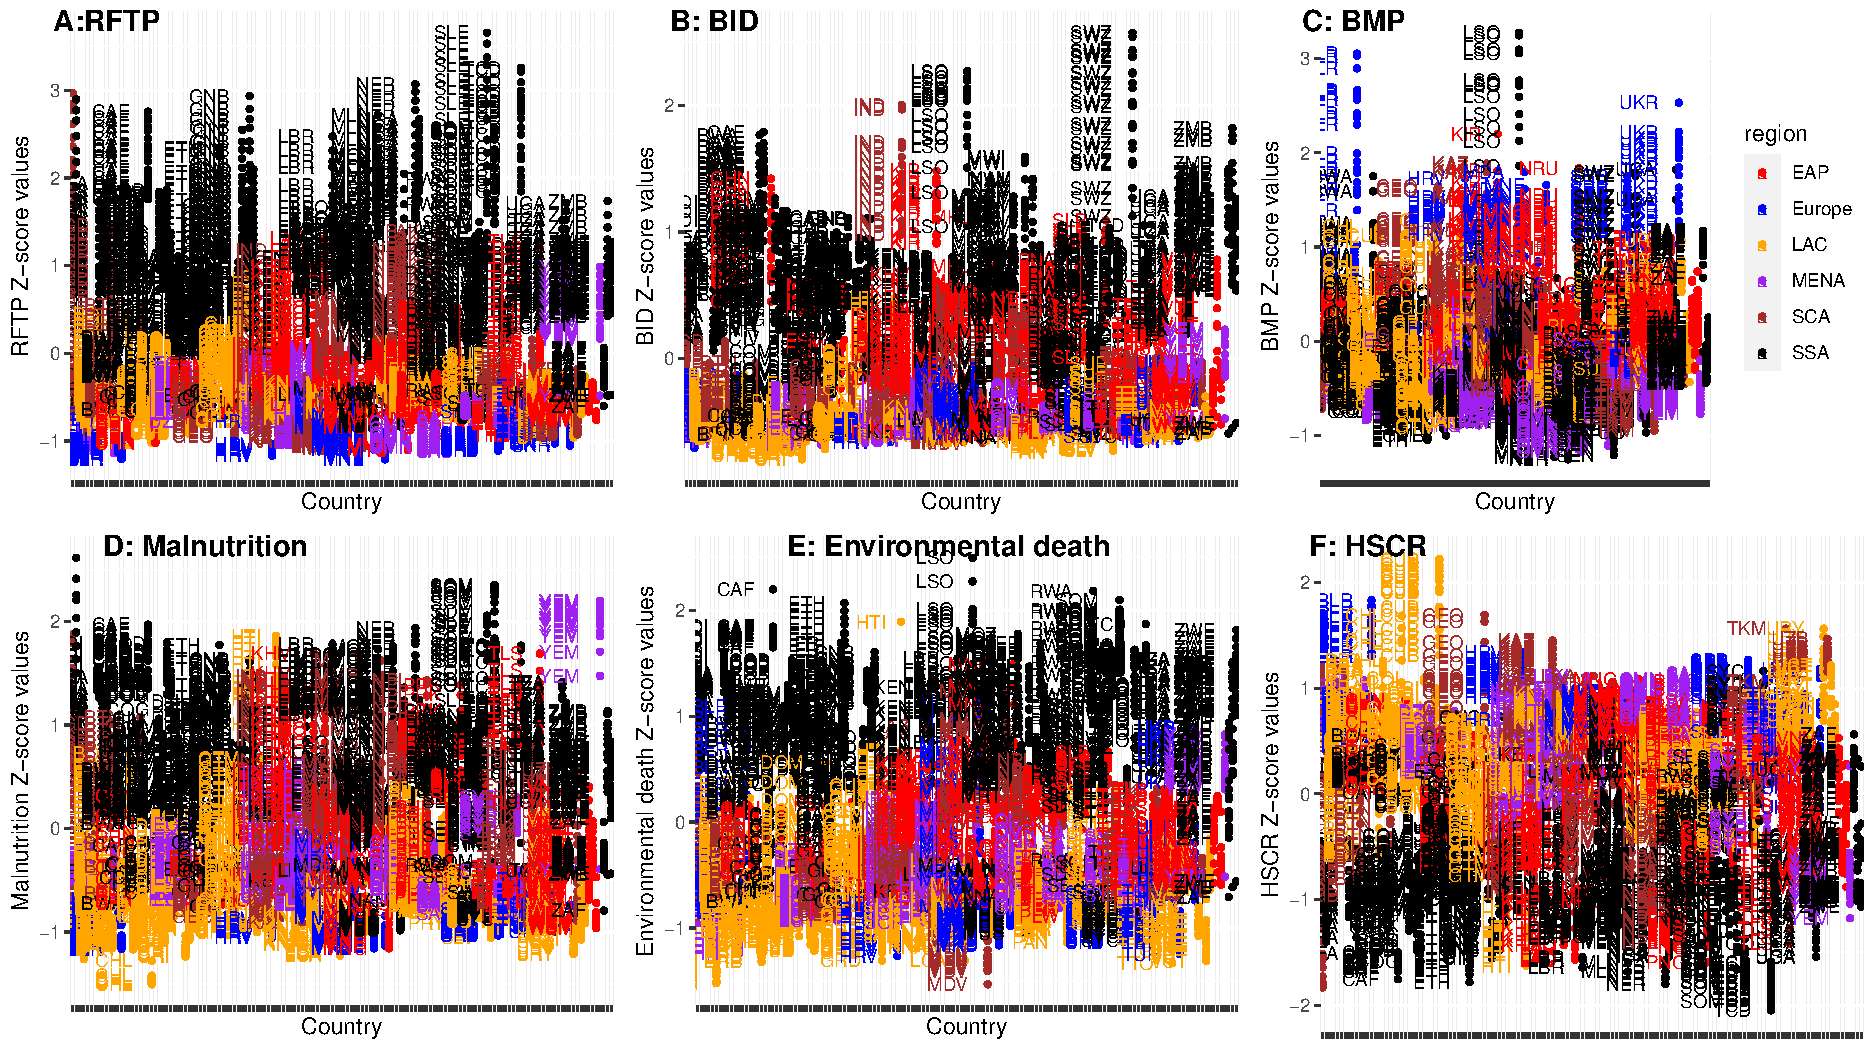
\includegraphics[width = 1.5\textwidth]{Figures/Health_Outcome_Graph/Combined_scatplot.pdf}
    \caption*{\footnotesize{Note. Reproductive health risk and mortality index comprises four indicators: maternal, under-5 child and neonatal mortality, and adolescent pregnancy incidence (10 to 19 years) access across the regions of interest. Author's computation, data from \textcite{unsdg_sustainable_2023, wdi_world_2023}}}
    \label{fig:combined_scat_plot}
\end{figure}
\end{landscape}

\subsubsection*{Appendix B.3: ODA Distribution}

\begin{figure}[H]
\captionsetup{justification=justified,singlelinecheck=false}
\caption{\textit{Global Highest Net ODA Recipients}}
    \centering 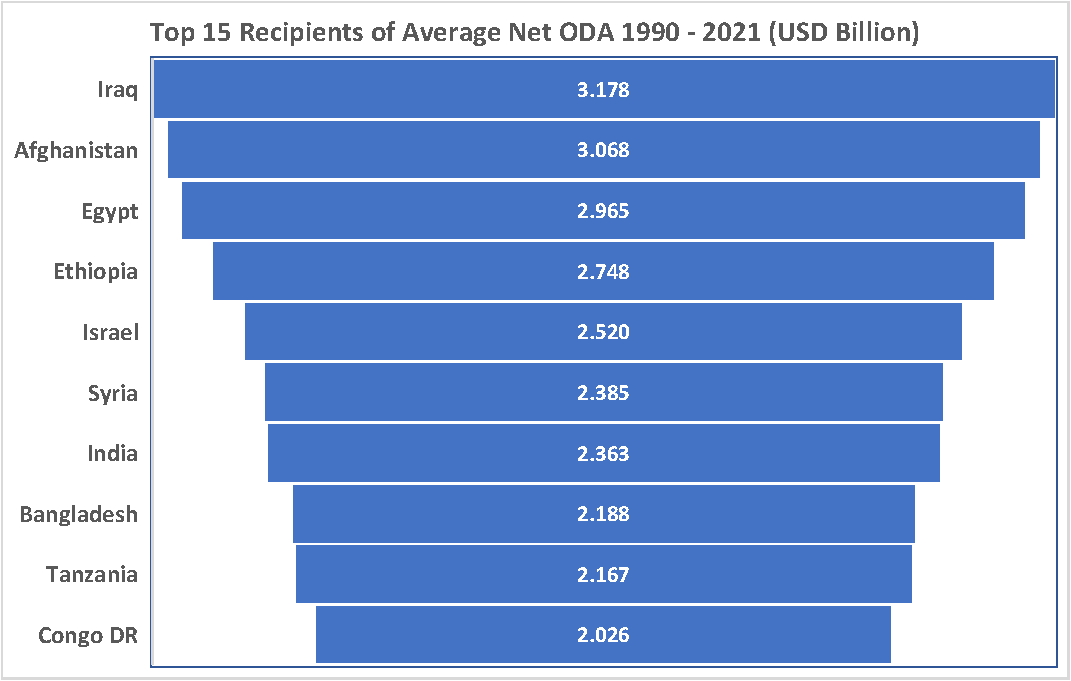
\includegraphics[width = 0.7\textwidth]{Figures/ODA_Graphs/Top_10_ODA_recps.pdf}
    \caption*{\footnotesize{Author's computation, data from \textcite{oecd_Data_2023}. Values are the average net ODA (2021 constant price) received between  1990 - 2021.}}
    \label{fig:ODA highest recipient}
\end{figure}



\begin{figure}[H]
\caption{\textit{Aid Dependency at Country Level}}
    \centering 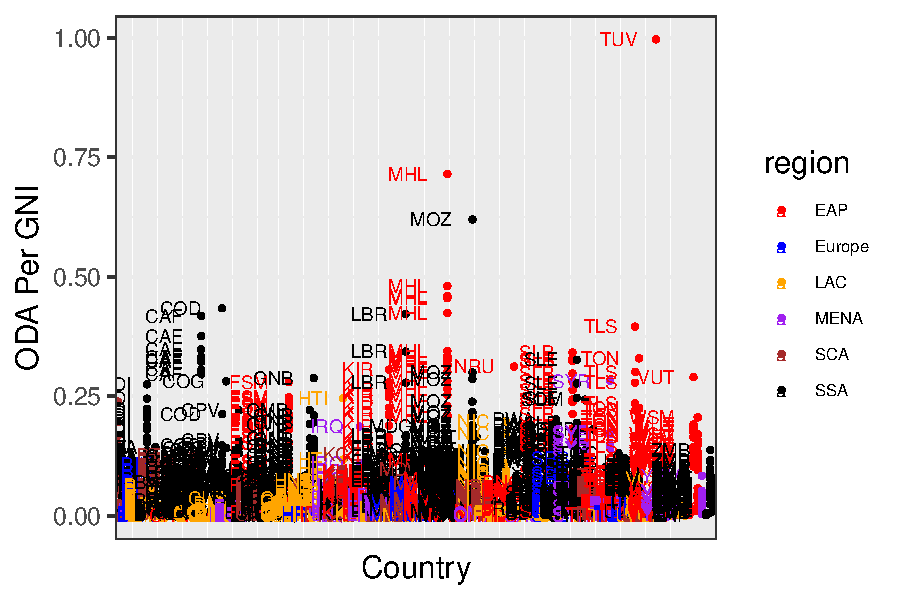
\includegraphics[width = 0.8\textwidth]{Figures/ODA_Graphs/ODA_GNI_scatPlot.pdf}
    \caption*{\footnotesize{Note. As mentioned above, there are outliers, with y-axis going up to 200\% as the dependency rate, showing the necessity for introducing log transformation applied in Fig \ref{fig:ODA Dependency by region}. Appropriate approaches will be introduced in later analysis. Percentage is the author's computation, with Net ODA at 2021 and GNI at 2015 constant price. Data from both \textcite{oecd_Data_2023, wdi_world_2023}}}
    \label{fig:aid dependency}
\end{figure}


\begin{figure}[H]
\captionsetup{justification=justified,singlelinecheck=false}
\caption{\textit{Relationship Between Social Infrastructure ODA and Various Health Dimensions}}
    \centering 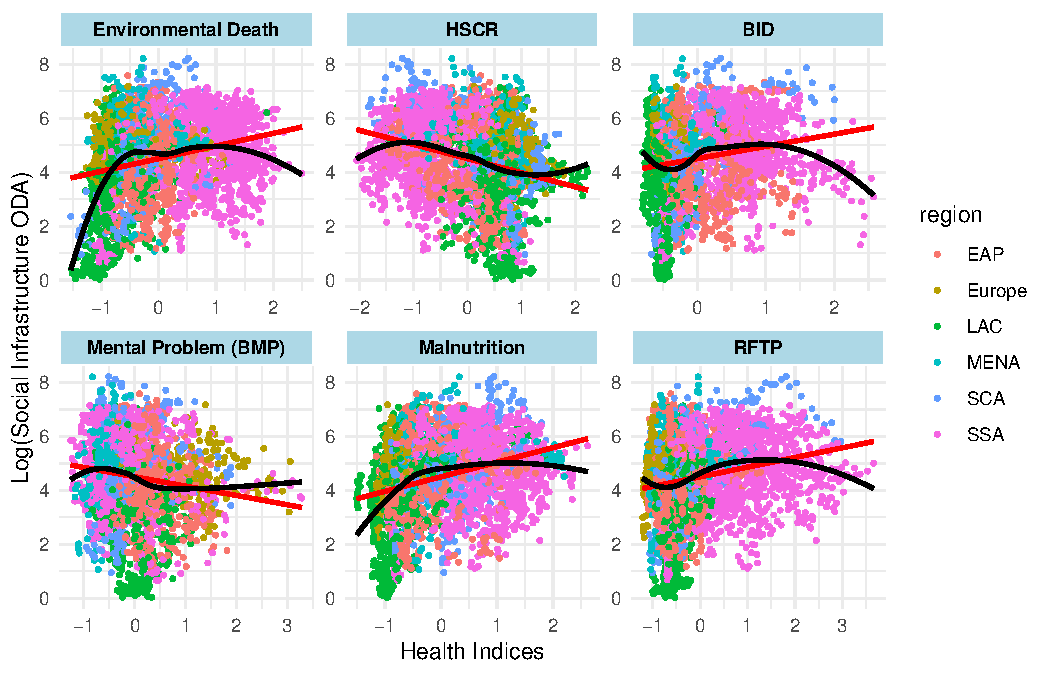
\includegraphics[width = 0.8\textwidth, height = 8cm]{Figures/ODA_against_Hth/Soc_ODA_Hth_plt.pdf}
    \label{fig:Social Infrastructure scatterplt}
    \caption*{\footnotesize{Note: Author's computation, data from \textcite{unsdg_sustainable_2023, wdi_world_2023}}}
\end{figure}


%\begin{figure}[ht]
%\captionsetup{justification=justified,singlelinecheck=false}
%\caption{Country Level Intensity of Reproductive Risk and Mortality}
%    \centering{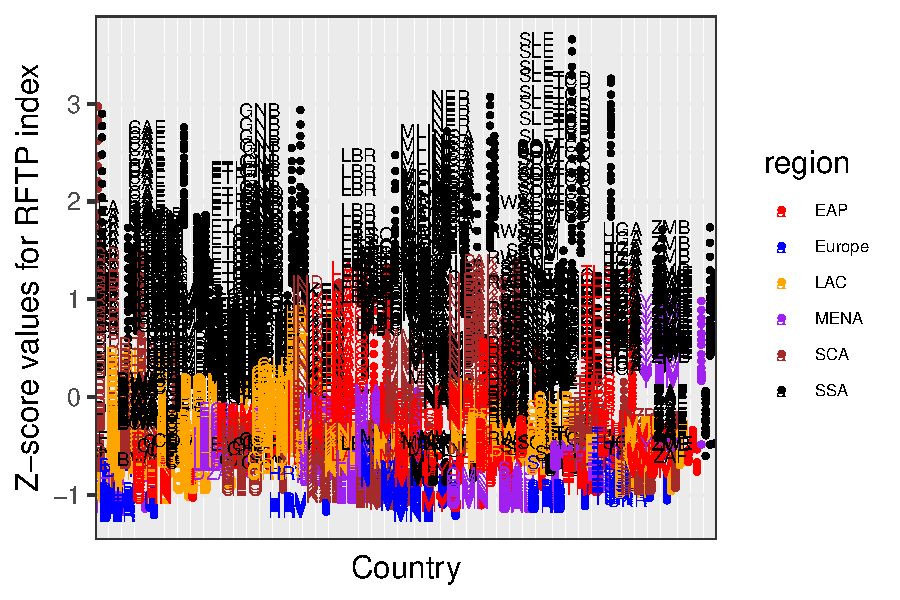
\includegraphics[width = 0.9\textwidth, height  = 7cm]{Figures/Health_Outcome_Graph/Reprod_Risks_scatPlot.pdf}}
 %   \label{fig:Reprod country scatplt}
  %  \caption*{\footnotesize{Author's computation, data from \textcite{oecd_Data_2023, unsdg_sustainable_2023, wdi_world_2023}.}}
%\end{figure}


%\begin{figure}[ht]
%\captionsetup{justification=justified,singlelinecheck=false}
%\caption{Country Level Mental Health Dimension}
 %   \centering{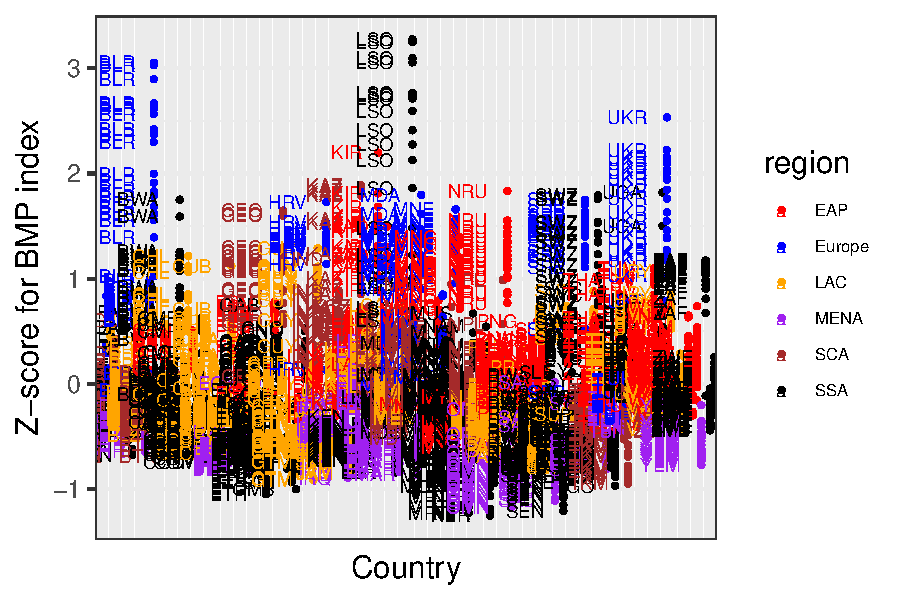
\includegraphics[width = 0.9\textwidth, height  = 7cm]{Figures/Health_Outcome_Graph/Mental_Hth_scatPlot.pdf}}
  %  \label{fig:Mental country scatplt}
   % \caption*{\footnotesize{Author's computation, data from \textcite{oecd_Data_2023, unsdg_sustainable_2023, wdi_world_2023}.}}
%\end{figure}

%\begin{figure}[ht]
%\captionsetup{justification=justified,singlelinecheck=false}
%\caption{Burden of Infections and Diseases at Country Level}
 %   \centering{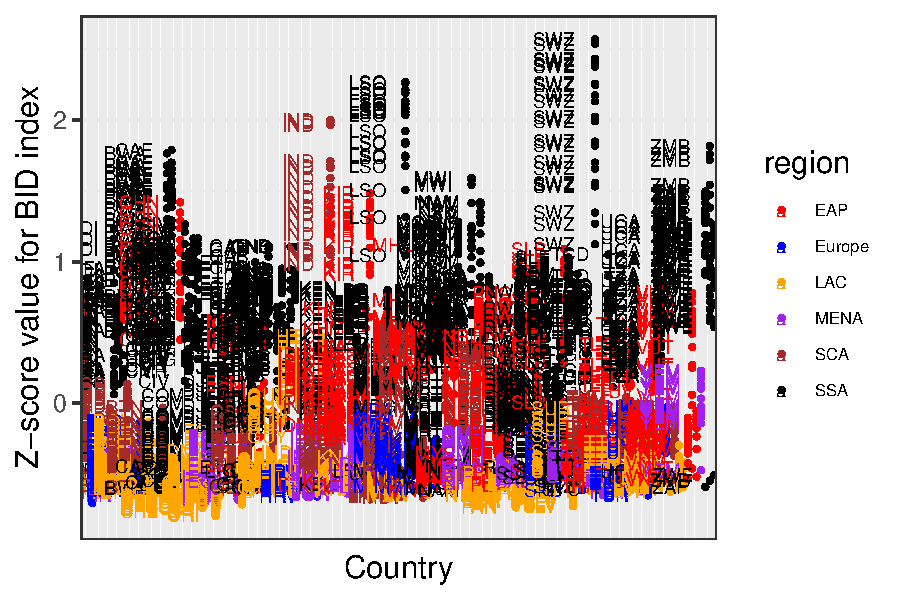
\includegraphics[width = 0.9\textwidth, height  = 7cm]{Figures/Health_Outcome_Graph/Burd_Infs_scatPlot.pdf}}
  %  \label{fig:Infection country scatplt}
   % \caption*{\footnotesize{Author's computation, data from \textcite{oecd_Data_2023, unsdg_sustainable_2023, wdi_world_2023}.}}
%\end{figure}

%\begin{figure}[ht]
%\captionsetup{justification=justified,singlelinecheck=false}
%\caption{Malnutrition Intensity at Country Level}
 %   \centering{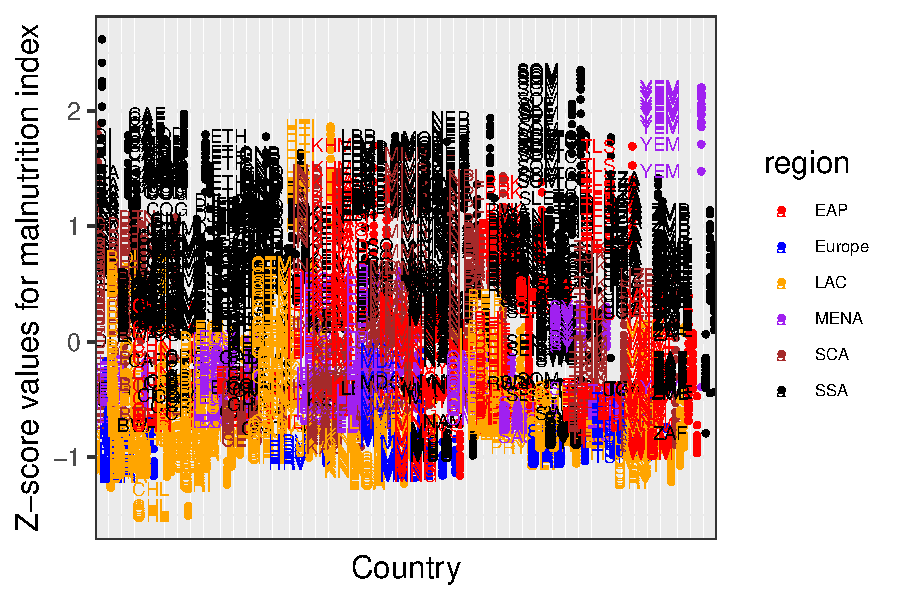
\includegraphics[width = 0.8\textwidth]{Figures/Health_Outcome_Graph/Malnutrition_scatPlot.pdf}}
  %  \label{fig:Malnutrition country scatplt}
   % \caption*{\footnotesize{Author's computation, data from \textcite{oecd_Data_2023, unsdg_sustainable_2023, wdi_world_2023}.}}
%\end{figure}


%\begin{figure}[ht]
%\captionsetup{justification=justified,singlelinecheck=false}
%\caption{Environmental Death at Country Level}
 %   \centering{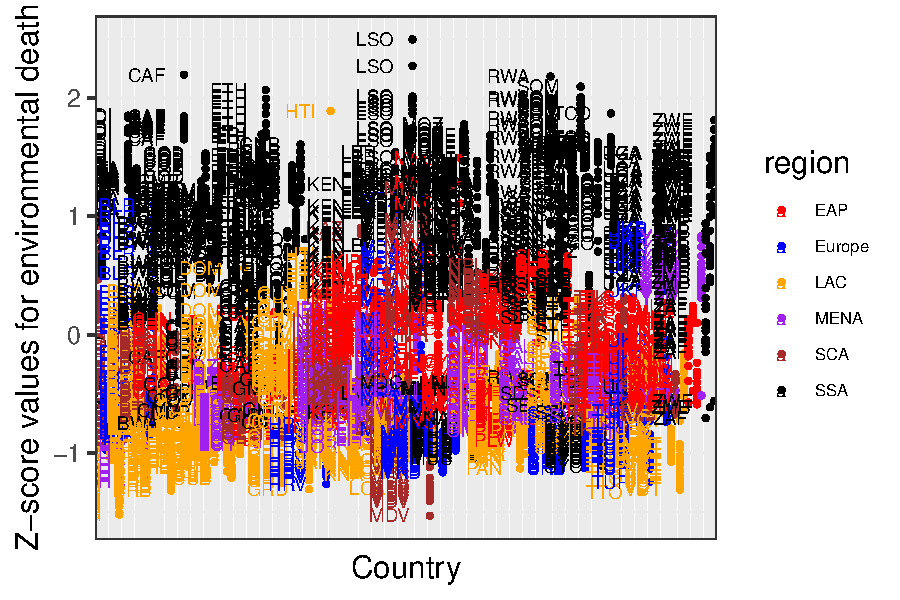
\includegraphics[width = 0.9\textwidth, height  = 7cm]{Figures/Health_Outcome_Graph/Env_death_scatPlot.pdf}}
  %  \label{fig:Env_death country scatplt}
   % \caption*{\footnotesize{Author's computation, data from \textcite{oecd_Data_2023, unsdg_sustainable_2023, wdi_world_2023}.}}
%\end{figure}



%\begin{figure}[ht]
%\captionsetup{justification=justified,singlelinecheck=false}
%\caption{Health System Capacity and Responsiveness at Country Level}
%    \centering{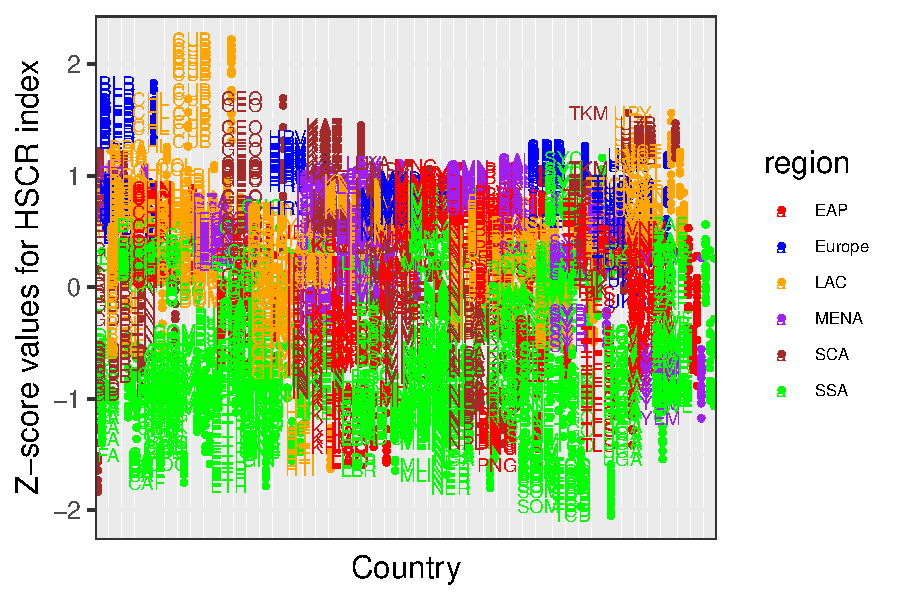
\includegraphics[width = 0.9\textwidth, height  = 7cm]{Figures/Health_Outcome_Graph/HSCR_scatPlot.pdf}}
 %   \label{fig:HSCR country scatplt}
 %   \caption*{\footnotesize{Author's computation, data from \textcite{oecd_Data_2023, unsdg_sustainable_2023, wdi_world_2023}.}}
%\end{figure}

%%%%%%% Statical Tests of 
\begin{figure}[H]
\captionsetup{justification=justified,singlelinecheck=false}
\caption{Correlation between ODA and Health Dimensions}
    \centering{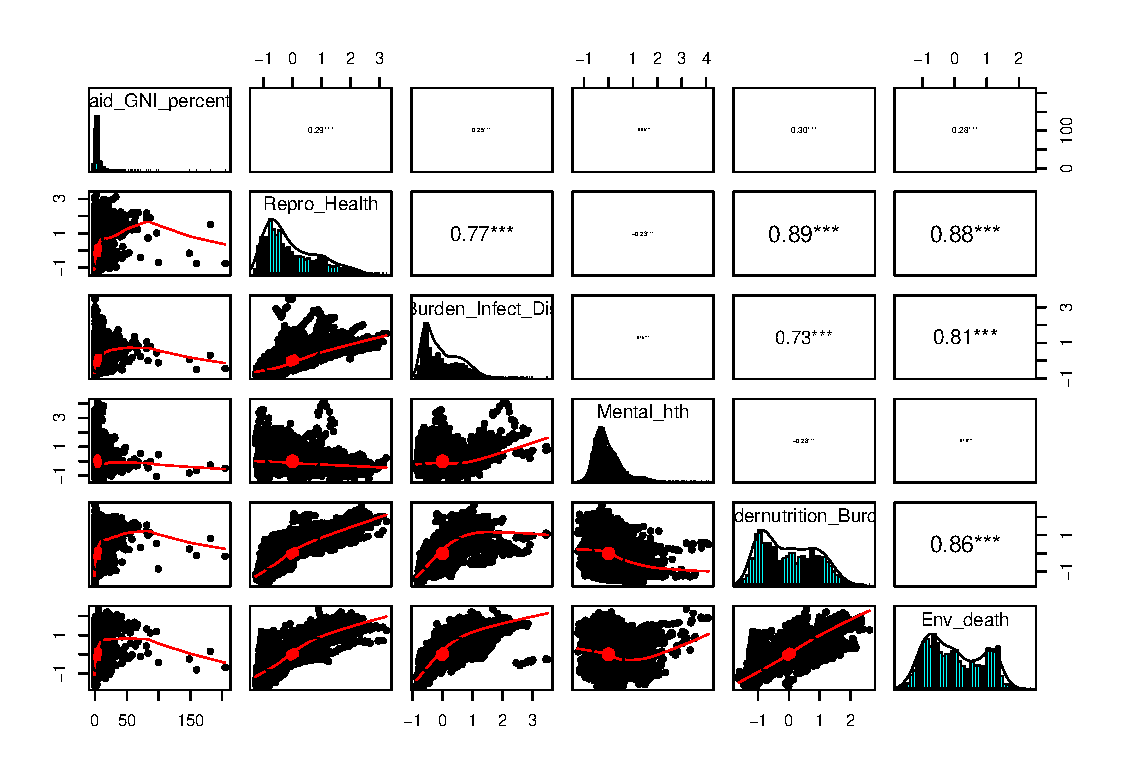
\includegraphics[width = 0.8\textwidth]{Figures/Health_Outcome_Graph/ODA_Hlth.pdf}}
    \label{fig:preliminary stat pair panels}
    \caption*{\footnotesize{Author's computation, data from \textcite{oecd_Data_2023, unsdg_sustainable_2023, wdi_world_2023}.}}
\label{Fig::Health_dimensions_correlation}
\end{figure}



\begin{figure}[H]
\captionsetup{justification=justified,singlelinecheck=false}
\caption{Correlation between ODA and Health Dimensions}
    \centering{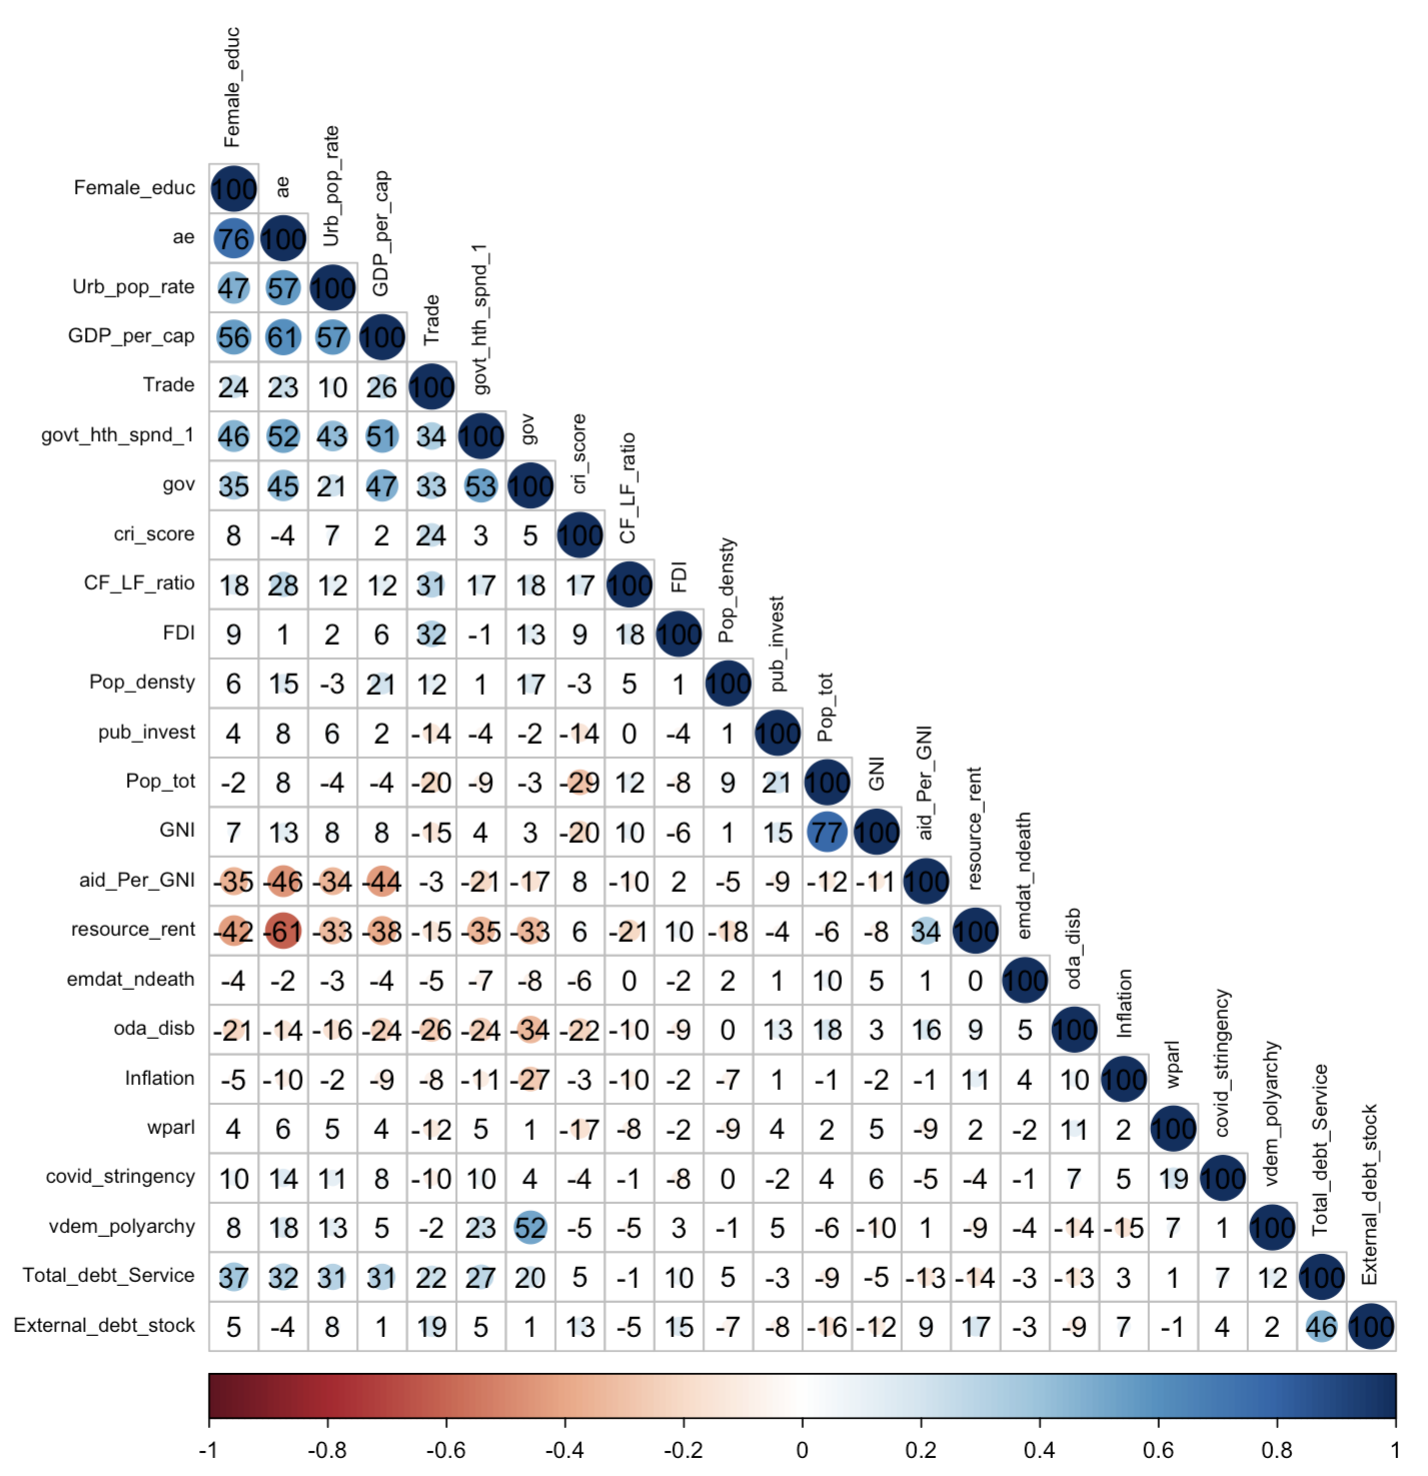
\includegraphics[width = 0.75\textwidth]{Results_outputs/Econometrics_Test/Multicolinearity_cor_graph.png}}
    \label{fig:Correlation_Matrix_Graph}
    \caption*{\footnotesize{Author's computation, data from \textcite{oecd_Data_2023, unsdg_sustainable_2023, wdi_world_2023}.}}
\end{figure}


\begin{figure}[H]

\caption{\textit{Social Infrastructure ODA and Social Protection Coverage}}
    \centering 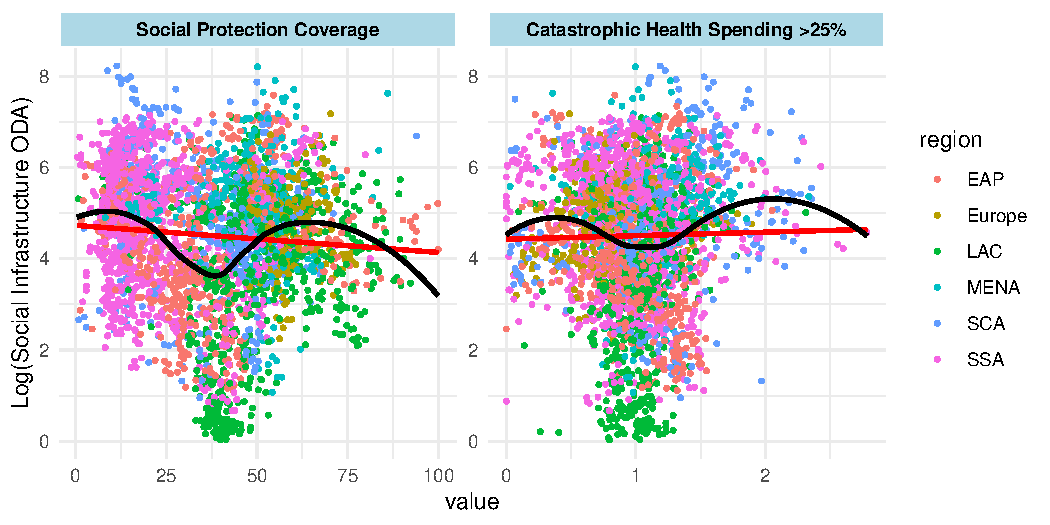
\includegraphics[width = 0.8\textwidth]{Figures/ODA_against_Hth/Soc_Prot_SocInfrODA_plt.pdf}
    \label{Fig::Social_Prot_Social_InfrastructureODA}
\end{figure}

\begin{figure}[H]
\captionsetup{justification=justified,singlelinecheck=false}
\caption{\textit{Total Net ODA and Social Protection Coverage}}
   \centering 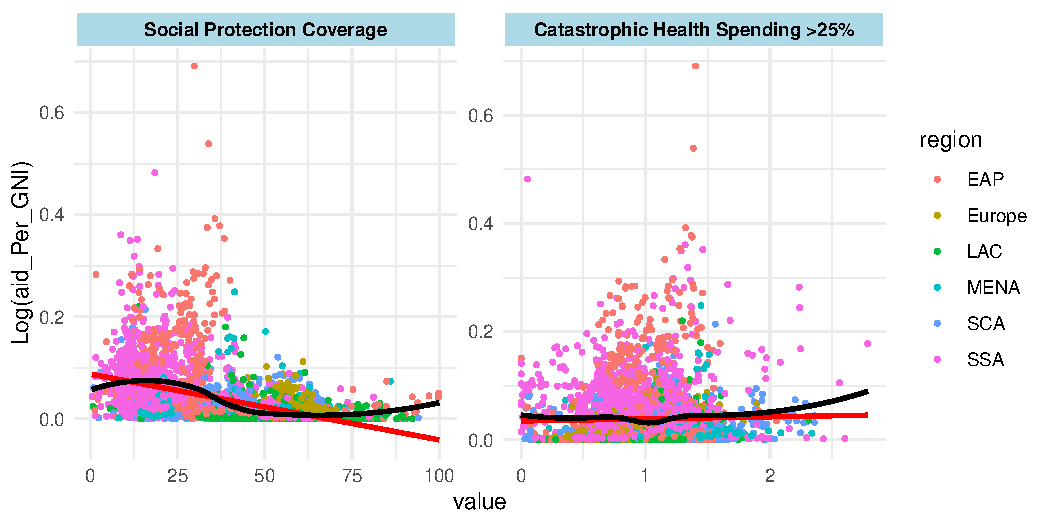
\includegraphics[width = 0.8\textwidth]{Figures/ODA_against_Hth/Soc_Prot_aid_Per_GNI_plt.pdf}
   \label{Fig::Social_Prot_Total_ODA}
\end{figure}



\subsection*{Appendix C.1: \quad Econometric Tests}
\addcontentsline{toc}{subsection}{Appendix C.1: Econometric Tests}

\begin{table}[H]
    \centering
    \caption{Descriptive Statistics for Variables}
    \begin{tabular}{lccccc}
    \toprule
\textbf{Variable} & \textbf{Max} & \textbf{Min} & \textbf{Mean} & \textbf{Median} & \textbf{SD} \\
    \midrule
oda\_disb & 13780.78 & 0.00 & 652.24 & 289.64 & 1014.71\\
aid\_Per\_GNI & 0.41 & 0.00 & 0.04 & 0.02 & 0.06\\

Soc\_Assistance\_cov & 89.52 & 3.91 & 28.76 & 27.80 & 14.30\\

SOC\_INF\_ODA & 3,145.69 & 0.33 & 214.37 & 113.09 & 296.06\\

Cov\_all\_SPL & 95.29 & 4.77 & 38.06 & 39.39 & 18.95\\
govt\_hth\_spnd\_1 & 96.24 & 4.47 & 44.42 & 44.30 & 18.94\\
GDP\_per\_cap & 48701.78 & 702.54 & 9594.26 & 7389.03 & 8244.58\\
Pop\_tot & 1.391656e+09 & 9634.00 & 39967530.32 & 9206846.50 & 151022305.31\\

Electricity\_access & 100 & 3.13 & 73.05 & 88.87 & 30.64\\
External\_debt\_stock & 453.55 & 1.28 & 56.81 & 49.67 & 42.46\\
Trade & 281.64 & 18.34 & 80.41 & 75.59 & 35.20\\
cri\_score & 127.72 & 8.33 & 81.39 & 85.15 & 23.83\\

gov & 1.23 & -2.40 & -0.43 & -0.43 & 0.62\\

FDI & 53.74 & -6.54 & 4.29 & 2.89 & 5.00\\

Pop\_densty & 1834.97 & 1.60 & 135.38 & 70.74 & 207.74\\

Zscore\_Reprd\_index & 3.46 & -1.19 & 0.00 & -0.32 & 0.91\\

Zscore\_Nutrit\_index & 2.37 & -1.50 & 0.00 & -0.17 & 0.83\\

Zscore\_EnvDeath\_index & 2.04 & -1.44 & 0.00 & -0.20 & 0.82\\

Zscore\_HSCR\_index & 2.18 & -1.91 & 0.00 & 0.12 & 0.80\\

Zscore\_InfDis\_index & 2.44 & -0.79 & 0.00 & -0.19 & 0.60\\

Zscore\_Mental\_index & 3.04 & -1.07 & 0.00 & -0.13 & 0.62\\
\bottomrule
\label{Tab::Stat_summary}
\end{tabular}
\end{table}


  \begin{table}[H]
    \centering
      \caption{Variance Inflation Factor (VIF) Results}
    \begin{tabular}{|l|c|}
        \hline
        \textbf{Variable} & \textbf{VIF Coefficients} \\
        \hline
        ODA & 2.216707 \\
        aid\_Per\_GNI & 1.456814 \\
        Soc\_Assistance\_cov & 4.264856 \\
        SOC\_INF\_ODA & 2.575421 \\
        govt\_hth\_spnd\_1 & 1.911189 \\
        GDP\_per\_cap & 2.199526 \\
        Pop\_tot & 1.381952 \\
        ae\_External\_debt\_stock & 2.943518 \\
        Trade & 1.094941 \\
        cri\_score & 1.496543 \\
        gov & 1.759377 \\
        FDI & 1.176758 \\
        Pop\_density & 1.169284 \\
        \hline
    \end{tabular}
    \label{tab:VIF_reslts}
\end{table}

\begin{table}[H]
    \centering
    \caption{Lagrange Multiplier Test - (Honda) for Country Specific Time-Fixed Effect}
    \begin{tabular}{lcc}
        \toprule
        \textbf{Model} & \textbf{Statistic} & \textbf{P-value} \\
        \midrule
        Reproductive Health & 25.886 & 2.2e-16 \\
        HSCR  & 25.594 & 2.2e-16 \\
        Environmental Death & 24.165 & 2.2e-16 \\
        Mental Health & 26.711 & 2.2e-16 \\
        Infection and Disease & 27.049 & 2.2e-16 \\
        Malnutrition & 25.087 & 2.2e-16 \\
        \bottomrule
    \end{tabular}
    \vspace{0.5em} % Add some space before the note
    \caption*{Note: The null hypothesis assumes no country-specific time fixed effect, a low P-value suggests rejection of the null hypothesis, indicating the significant difference in each country's coefficients.}
    \label{Tab::UnitFE_Test}
\end{table}


\begin{table}[H]
    \centering
    \caption{Lagrange Multiplier Test - (Honda) for Country Specific Time-Fixed Effect}
    \begin{tabular}{lcc}
        \toprule
        \textbf{Model} & \textbf{Statistic} & \textbf{P-value} \\
        \midrule
        Reproductive Health & 0.046913 & 0.4813 \\
        HSCR  & -0.58512 & 0.7208 \\
        Environmental Death & -1.2808 & 0.8999 \\
        Mental Health & 1.6818 & 0.04631 \\
        Infection and Disease & -1.2764 & 0.8991 \\
        Malnutrition & 1.0619 & 0.1441 \\
        \bottomrule
    \end{tabular}
    \vspace{0.5em} % Add some space before the note
    \caption*{Note: The null hypothesis, p > 5\%, assumes no time-varying common shock effect. Since the p-value> 5\% for all models, except the mental problem, we fail to reject the null hypothesis, thus, no time effect.}
    \label{Tab::TimeFE_test}
\end{table}


\begin{table}[H]
    \centering
    \caption{Breusch-Pagan Test Results for Heteroskedasticity}
    \begin{tabular}{lccc}
        \toprule
        \textbf{Model} & \textbf{BP Statistic} & \textbf{df} & \textbf{P-value} \\
        \midrule
        Reproductive Health & 169.2 & 13 & $< 2.2 \times 10^{-16}$ \\
        HSCR (Health, Safety, and Child Rights) & 55.348 & 13 & $3.51 \times 10^{-07}$ \\
        Environmental Health & 84.453 & 13 & $1.591 \times 10^{-12}$ \\
        Mental Health & 67.146 & 13 & $2.68 \times 10^{-09}$ \\
        Infectious Disease & 35.373 & 13 & 0.000742 \\
        Nutritional Health & 38.087 & 13 & 0.0002793 \\
        \bottomrule
    \end{tabular}
    \vspace{0.5em} % Add some space before the note
    \caption*{Note: The null hypothesis assumes homoskedasticity, and a low P-value suggests rejection of the null hypothesis, indicating the presence of heteroskedasticity in the model residuals.}
    \label{Tab::Heteroskedict}
\end{table}

%\begin{table}[ht]
    \centering
    \caption{Pesaran CD test for cross-sectional dependence in panels}
    \begin{tabular}{lcc}
        \toprule
        \textbf{Model} & \textbf{E} & \textbf{Estimates} \\
        \midrule
        Reproductive Health & z = -0.73509, p-value = 0.4623 \\
        HSCR  & 2.2118, p-value = 0.02698 \\
        Environmental Death  & z = 9.4918, p-value < 2.2e-16 \\
        Mental Health & z = 0.51595, p-value = 0.6059 \\
        Infection and Disease  & z = 6.0353, p-value = 1.587e-09 \\
        Malnutrition & z = 22.848, p-value < 2.2e-16 \\
        \bottomrule
    \end{tabular}
    \vspace{0.5em} % Add some space before the note
    \caption*{Note: The null hypothesis, p > 5\%, assumes no time-varying common shock effect. Since the p-value> 5\% for all models, except the mental problem, we fail to reject the null hypothesis, thus, no time effect.}
    \label{Tab::Cross_sect_depen_test}
\end{table}


\begin{table}[H]
    \centering
    \caption{BreuschGodfrey/Wooldridge Test for Serial Correlation in Panel}
    \begin{tabular}{lc}
        \toprule
        \textbf{Model} & \textbf{Serial Correlation}  \\
        \midrule
        Reproductive Health & $\chi^2 = 104.2, df = 4, p-value < 2.2e-16$  \\
        HSCR  & $ \chi^2 = 90.509, df = 4, p-value < 2.2e-16$ \\
        Environmental Death & $\chi^2 = 104.79, df = 4, p-value < 2.2e-16 $ \\
        Mental Health & $\chi^2 = 101.38, df = 4, p-value < 2.2e-16 $\\
        Infection and Disease & $\chi^2 = 128.29, df = 4, p-value < 2.2e-16$  \\
        Malnutrition & $\chi^2 = 119.56, df = 4, p-value < 2.2e-16$  \\
        \bottomrule
    \end{tabular}
    \vspace{0.5em} % Add some space before the note
    \caption*{Note: The null hypothesis, p $>$ 5\%, assumes no time-varying common shock effect. Since the p-value $>$ 5\% for all models, except the mental problem, we fail to reject the null hypothesis, thus, no time effect.}
    \label{Tab::Serial_corr_Test}
\end{table}




%\begin{table}[ht]
    \centering
    \caption{Lagrange Multiplier Test Results for Individual and Time Effects}
    \begin{tabular}{lcccccc}
        \toprule
        \textbf{Model} & \textbf{Chisq Statistic} & \textbf{df0} & \textbf{df1} & \textbf{df2} & \textbf{P-value} \\
        \midrule
        Reproductive Health & 999.09 & 0.00 & 1.00 & 2.00 & $< 2.2 \times 10^{-16}$ \\
        HSCR & 728.05 & 0.00 & 1.00 & 2.00 & $< 2.2 \times 10^{-16}$ \\
        Environmental Health & 901.97 & 0.00 & 1.00 & 2.00 & $< 2.2 \times 10^{-16}$ \\
        Mental Health & 1149.3 & 0.00 & 1.00 & 2.00 & $< 2.2 \times 10^{-16}$ \\
        Infectious Disease & 1161.1 & 0.00 & 1.00 & 2.00 & $< 2.2 \times 10^{-16}$ \\
        Nutritional Health & 953.23 & 0.00 & 1.00 & 2.00 & $< 2.2 \times 10^{-16}$ \\
        \bottomrule
    \end{tabular}
    \vspace{0.5em} % Add some space before the note
    \caption*{Note: The null hypothesis assumes no individual and time effects. A low P-value suggests rejection of the null hypothesis, indicating the presence of significant effects.}
    \label{Tab::Panel_Test}
\end{table}

%\begin{table}[H]
    \centering
    \caption{Breusch-Pagan Test Results for Heteroskedasticity}
    \begin{tabular}{lccc}
        \toprule
        \textbf{Model} & \textbf{BP Statistic} & \textbf{df} & \textbf{P-value} \\
        \midrule
        Reproductive Health & 169.2 & 13 & $< 2.2 \times 10^{-16}$ \\
        HSCR (Health, Safety, and Child Rights) & 55.348 & 13 & $3.51 \times 10^{-07}$ \\
        Environmental Health & 84.453 & 13 & $1.591 \times 10^{-12}$ \\
        Mental Health & 67.146 & 13 & $2.68 \times 10^{-09}$ \\
        Infectious Disease & 35.373 & 13 & 0.000742 \\
        Nutritional Health & 38.087 & 13 & 0.0002793 \\
        \bottomrule
    \end{tabular}
    \vspace{0.5em} % Add some space before the note
    \caption*{Note: The null hypothesis assumes homoskedasticity, and a low P-value suggests rejection of the null hypothesis, indicating the presence of heteroskedasticity in the model residuals.}
    \label{Tab::Heteroskedict}
\end{table}


 

%\newpage
\subsection*{Appendix D: List of Countries and Respective Regions}
\addcontentsline{toc}{subsection}{Appendix D: List of Countries and Respective Regions}


% latex table generated in R 4.3.2 by xtable 1.8-4 package
% Sun Dec 24 15:21:07 2023
\afterpage{
\begin{longtable}{l l c c}
\caption{List of Countries and Regions} 
  \hline  \\[-2ex]
    \textbf{No.} & \textbf{Country name} & \textbf{Iso3c codes} & \textbf{Regions} \\ 
  \hline  \\[-0.8ex]
1 & Afghanistan & AFG & SCA \\ 
  2 & Angola & AGO & SSA \\ 
  3 & Albania & ALB & Europe \\ 
  4 & Argentina & ARG & LAC \\ 
  5 & Armenia & ARM & SCA \\ 
  6 & Antigua and Barbuda & ATG & LAC \\ 
  7 & Azerbaijan & AZE & SCA \\ 
  8 & Burundi & BDI & SSA \\ 
  9 & Benin & BEN & SSA \\ 
  10 & Burkina Faso & BFA & SSA \\ 
  11 & Bangladesh & BGD & SCA \\ 
  12 & Bahrain & BHR & MENA \\ 
  13 & Bosnia and Herzegovina & BIH & Europe \\ 
  14 & Belarus & BLR & Europe \\ 
  15 & Belize & BLZ & LAC \\ 
  16 & Bolivia & BOL & LAC \\ 
  17 & Brazil & BRA & LAC \\ 
  18 & Barbados & BRB & LAC \\ 
  19 & Bhutan & BTN & SCA \\ 
  20 & Botswana & BWA & SSA \\ 
  21 & Central African Republic & CAF & SSA \\ 
  22 & Chile & CHL & LAC \\ 
  23 & China (People's Republic of) & CHN & EAP \\ 
  24 & Côte d'Ivoire & CIV & SSA \\ 
  25 & Cameroon & CMR & SSA \\ 
  26 & Democratic Republic of the Congo & COD & SSA \\ 
  27 & Congo & COG & SSA \\ 
  28 & Colombia & COL & LAC \\ 
  29 & Comoros & COM & SSA \\ 
  30 & Cabo Verde & CPV & SSA \\ 
  31 & Costa Rica & CRI & LAC \\ 
  32 & Cuba & CUB & LAC \\ 
  33 & Djibouti & DJI & SSA \\ 
  34 & Dominica & DMA & LAC \\ 
  35 & Dominican Republic & DOM & LAC \\ 
  36 & Algeria & DZA & MENA \\ 
  37 & Ecuador & ECU & LAC \\ 
  38 & Egypt & EGY & MENA \\ 
  39 & Eritrea & ERI & SSA \\ 
  40 & Ethiopia & ETH & SSA \\ 
  41 & Fiji & FJI & EAP \\ 
  42 & Micronesia & FSM & EAP \\ 
  43 & Gabon & GAB & SSA \\ 
  44 & Georgia & GEO & SCA \\ 
  45 & Ghana & GHA & SSA \\ 
  46 & Guinea & GIN & SSA \\ 
  47 & Gambia & GMB & SSA \\ 
  48 & Guinea-Bissau & GNB & SSA \\ 
  49 & Equatorial Guinea & GNQ & SSA \\ 
  50 & Grenada & GRD & LAC \\ 
  51 & Guatemala & GTM & LAC \\ 
  52 & Guyana & GUY & LAC \\ 
  53 & Honduras & HND & LAC \\ 
  54 & Croatia & HRV & Europe \\ 
  55 & Haiti & HTI & LAC \\ 
  56 & Indonesia & IDN & EAP \\ 
  57 & India & IND & SCA \\ 
  58 & Iran & IRN & MENA \\ 
  59 & Iraq & IRQ & MENA \\ 
  60 & Jamaica & JAM & LAC \\ 
  61 & Jordan & JOR & MENA \\ 
  62 & Kazakhstan & KAZ & SCA \\ 
  63 & Kenya & KEN & SSA \\ 
  64 & Kyrgyzstan & KGZ & SCA \\ 
  65 & Cambodia & KHM & EAP \\ 
  66 & Kiribati & KIR & EAP \\ 
  67 & Saint Kitts and Nevis & KNA & LAC \\ 
  68 & Lao People's Democratic Republic & LAO & EAP \\ 
  69 & Lebanon & LBN & MENA \\ 
  70 & Liberia & LBR & SSA \\ 
  71 & Libya & LBY & MENA \\ 
  72 & Saint Lucia & LCA & LAC \\ 
  73 & Sri Lanka & LKA & SCA \\ 
  74 & Lesotho & LSO & SSA \\ 
  75 & Morocco & MAR & MENA \\ 
  76 & Moldova & MDA & Europe \\ 
  77 & Madagascar & MDG & SSA \\ 
  78 & Maldives & MDV & SCA \\ 
  79 & Mexico & MEX & LAC \\ 
  80 & Marshall Islands & MHL & EAP \\ 
  81 & North Macedonia & MKD & Europe \\ 
  82 & Mali & MLI & SSA \\ 
  83 & Myanmar & MMR & SCA \\ 
  84 & Montenegro & MNE & Europe \\ 
  85 & Mongolia & MNG & EAP \\ 
  86 & Mozambique & MOZ & SSA \\ 
  87 & Mauritania & MRT & SSA \\ 
  88 & Mauritius & MUS & SSA \\ 
  89 & Malawi & MWI & SSA \\ 
  90 & Malaysia & MYS & EAP \\ 
  91 & Namibia & NAM & SSA \\ 
  92 & Niger & NER & SSA \\ 
  93 & Nigeria & NGA & SSA \\ 
  94 & Nicaragua & NIC & LAC \\ 
  95 & Nepal & NPL & SCA \\ 
  96 & Nauru & NRU & EAP \\ 
  97 & Oman & OMN & MENA \\ 
  98 & Pakistan & PAK & SCA \\ 
  99 & Panama & PAN & LAC \\ 
  100 & Peru & PER & LAC \\ 
  101 & Philippines & PHL & EAP \\ 
  102 & Palau & PLW & EAP \\ 
  103 & Papua New Guinea & PNG & EAP \\ 
  104 & Democratic People's Republic of Korea & PRK & EAP \\ 
  105 & Paraguay & PRY & LAC \\ 
  106 & Rwanda & RWA & SSA \\ 
  107 & Saudi Arabia & SAU & MENA \\ 
  108 & Sudan & SDN & SSA \\ 
  109 & Senegal & SEN & SSA \\ 
  110 & Solomon Islands & SLB & EAP \\ 
  111 & Sierra Leone & SLE & SSA \\ 
  112 & El Salvador & SLV & LAC \\ 
  113 & Somalia & SOM & SSA \\ 
  114 & Serbia & SRB & Europe \\ 
  115 & Sao Tome and Principe & STP & SSA \\ 
  116 & Suriname & SUR & LAC \\ 
  117 & Eswatini & SWZ & SSA \\ 
  118 & Seychelles & SYC & SSA \\ 
  119 & Syrian Arab Republic & SYR & MENA \\ 
  120 & Chad & TCD & SSA \\ 
  121 & Togo & TGO & SSA \\ 
  122 & Thailand & THA & EAP \\ 
  123 & Tajikistan & TJK & SCA \\ 
  124 & Turkmenistan & TKM & SCA \\ 
  125 & Timor-Leste & TLS & EAP \\ 
  126 & Tonga & TON & EAP \\ 
  127 & Trinidad and Tobago & TTO & LAC \\ 
  128 & Tunisia & TUN & MENA \\ 
  129 & Türkiye & TUR & Europe \\ 
  130 & Tuvalu & TUV & EAP \\ 
  131 & Tanzania & TZA & SSA \\ 
  132 & Uganda & UGA & SSA \\ 
  133 & Ukraine & UKR & Europe \\ 
  134 & Uruguay & URY & LAC \\ 
  135 & Uzbekistan & UZB & SCA \\ 
  136 & Saint Vincent and the Grenadines & VCT & LAC \\ 
  137 & Venezuela & VEN & LAC \\ 
  138 & Viet Nam & VNM & EAP \\ 
  139 & Vanuatu & VUT & EAP \\ 
  140 & Samoa & WSM & EAP \\ 
  141 & Yemen & YEM & MENA \\ 
  142 & South Africa & ZAF & SSA \\ 
  143 & Zambia & ZMB & SSA \\ 
  144 & Zimbabwe & ZWE & SSA \\ 
   \hline
\label{tab:country_info}
\end{longtable}

}


% Include other appendices as needed
\newpage
% Bibliography

\printbibliography
\addcontentsline{toc}{section}{REFERENCES}
%https://cran.r-project.org/web/packages/dotwhisker/vignettes/dotwhisker-vignette.html
%https://mpra.ub.uni-muenchen.de/62350/1/MPRA_paper_62350.pdf
%https://journals.sagepub.com/doi/full/10.1177/2378023117710578
\end{document}


